%%%%%%%%%%%%%%%%%%%%%%%%%%%%%%%%%%%%%%%%%%%%%%%%%%%
%% LaTeX book template                           %%
%% Author:  Amber Jain (http://amberj.devio.us/) %%
%% License: ISC license                          %%
%%%%%%%%%%%%%%%%%%%%%%%%%%%%%%%%%%%%%%%%%%%%%%%%%%%

\documentclass[a4paper,11pt,oneside]{book}

% pacotes utilizados
\usepackage[T1]{fontenc}
\usepackage[utf8]{inputenc}
\usepackage{lmodern}
\usepackage{hyperref}
\usepackage{graphicx}
\usepackage[portuguese]{babel}
\usepackage{amsfonts}
\usepackage[usenames,dvipsnames]{xcolor}
\usepackage{mathtools}
\usepackage{amssymb} % alguns simbolos matematicos
\usepackage{mathrsfs} % letras cursivas
\usepackage{listings} % coding examples in latex file
\usepackage{xcolor} % changing colors
\usepackage{amsthm} % definir estilo do teorema
\usepackage[hang,flushmargin]{footmisc} % remove footnote's identation
\usepackage{cancel} % para poder colocar o tracinho de cancelamento
\usepackage{tikz} % to draw Venn's diagrams
\usepackage{amsmath} % to write a function by cases
\usepackage{graphicx} % to set a images directory
\usepackage{caption} % to supress numbering in figures
\usepackage{float} % to make a figure stay when i whant
\usepackage{sgame} % to make payoff matrixes
\usepackage{qtree} % to make tree diagrams

\usepackage[shortrightarrow]{stmaryrd} % shortarrow

\graphicspath{{./images/}} % set an default images folder

% dark theme no pdf
\pagecolor[rgb]{0.1,0.1,0.1} %black
\color[rgb]{0.9,0.9,0.9} %grey

% criando o modelo de definicoes/teoremas/fatos/demonstracoes
\theoremstyle{definition}

\newtheoremstyle{break}% name
  {10pt}%         Space above, empty = `usual value'
  {10pt}%         Space below
  {}% Body font
  {}%         Indent amount (empty = no indent, \parindent = para indent)
  {\bfseries}% Thm head font
  {}%        Punctuation after thm head
  {\newline}% Space after thm head: \newline = linebreak
  {}%         Thm head spec

\theoremstyle{break}

% definindo as categorias de formalidade
\newtheorem{definition}{Definição}[section]
\newtheorem{fact}{Fato}[section]
\newtheorem{demonstration}{Demonstração}[section]
\newtheorem{theorem}{Teorema}

% tirando identação dos paragrafos
\setlength{\parindent}{0ex}

% setting das cores quando usar codigo python
\definecolor{codegreen}{rgb}{0,0.6,0}
\definecolor{codegray}{rgb}{0.5,0.5,0.5}
\definecolor{codepurple}{rgb}{0.58,0,0.82}
\definecolor{backcolour}{rgb}{0.95,0.95,0.92}

\lstdefinestyle{mystyle}{
    backgroundcolor=\color{backcolour},   
    commentstyle=\color{codegreen},
    keywordstyle=\color{magenta},
    numberstyle=\tiny\color{codegray},
    stringstyle=\color{codepurple},
    basicstyle=\ttfamily\footnotesize,
    breakatwhitespace=false,         
    breaklines=true,                 
    captionpos=b,                    
    keepspaces=true,                 
    numbers=left,                    
    numbersep=5pt,                  
    showspaces=false,                
    showstringspaces=false,
    showtabs=false,                  
    tabsize=2
}

\lstset{style=mystyle}

% dedicatoria 
% Source: http://www.tug.org/pipermail/texhax/2010-June/
\newenvironment{dedication}
{
   \cleardoublepage
   \thispagestyle{empty}
   \vspace*{\stretch{1}}
   \hfill\begin{minipage}[t]{0.66\textwidth}
   \raggedright
}
{
   \end{minipage}
   \vspace*{\stretch{3}}
   \clearpage
}

% Chapter quote at the start of chapter        %
% Source: http://tex.stackexchange.com/a/53380 %
\makeatletter
\renewcommand{\@chapapp}{}% Not necessary...
\newenvironment{chapquote}[2][2em]
  {\setlength{\@tempdima}{#1}%
   \def\chapquote@author{#2}%
   \parshape 1 \@tempdima \dimexpr\textwidth-2\@tempdima\relax%
   \itshape}
  {\par\normalfont\hfill--\ \chapquote@author\hspace*{\@tempdima}\par\bigskip}
\makeatother

%%%%%%%%%%%%%%%%%%%%%%%%%%%%%%%%%%%%%%%%%%%%%%%%%%%
% First page of book which contains 'stuff' like: %
%  - Book title, subtitle                         %
%  - Book author name                             %
%%%%%%%%%%%%%%%%%%%%%%%%%%%%%%%%%%%%%%%%%%%%%%%%%%%
% Book's title and subtitle
\title{\Huge \textbf{Microeconomia} \\ 
\Large Tradução da 9 edição \\
\huge Hal R. Varian}

% Author
\author{
\textsc{Resumo e Adaptação por:} \\
\textsc{Bruno de M. Ruas}
}

\begin{document}

\frontmatter
\maketitle

\tableofcontents
%\listoffigures
%\listoftables

\mainmatter

%%%%%%%%%%%%%%%%%%%%%%%% PART %%%%%%%%%%%%%%%%%%%%%%%%
\part*{Preparativos}
\addcontentsline{toc}{part}{Preparativos}

%%%%%%%%%%%%%%%%%%%%%%%% CHAPTER %%%%%%%%%%%%%%%%%%%%%%%%
\chapter*{Matemática}
\addcontentsline{toc}{chapter}{Matemática}

\begin{chapquote}{The Godfather}
	``Some Day, And That Day May Never Come, I Will Call Upon You To Do A Service For Me.''.
\end{chapquote}

Bem vindo ao meu resumo do livro do prof. Varian. Ao contrário do que ele fez, eu preferi trazer o apêndice de matemática pro começo do material porque aqui nós vamos ver as ferramentas que serão usadas para a explicação dos conceitos teóricos ao longo do material.
\\
\\
Aqui a gente só vai dar um overview básico nos conceitos. Não tenha dúvida que alguém mais experimentado em matemática torceria o nariz pra algumas definições dadas aqui. Mas o objetivo é te dar um "norte"\ a respeito de alguns conceitos normalmente usados. Não se assuste com a simplicidade de algumas coisas. Melhor garantir agora do que sofrer mais pra frente no texto.

\section*{Funções}
\addcontentsline{toc}{section}{Funções}

Sejam dois números quaisquer $x$ e $y$, uma \textbf{função} ou \textbf{transformação} é uma regra que descreve uma relação entre eles.
\\
\\
Para demonstrar que existe alguma dependência entre duas variáveis usamos a notação $y = f(x)$, onde nossa variável $y$ (chamada de \textbf{dependente}) é o resultado de alguma transformação (denotada pelo símbolo $"f"$) realizada em $x$ (nossa variável \textbf{independente}).
\\
\\
Não é raro ter uma variável dependente relacionada a várias outras variáveis. Nesses casos é comum o uso da notação anterior com a adição das novas incógnitas. Algo como $y = f(x_1,x_2,...,x_n)$.

\section*{Gráficos}
\addcontentsline{toc}{section}{Gráficos}

Não tem muito o que falar aqui. Dá uma lida lá na página 1010.

\section*{Propriedades das Funções}
\addcontentsline{toc}{section}{Propriedades das Funções}

Uma função pode ter algumas características que facilitam a sua descrição. Aqui temos algumas que serão usadas ao longo do curso:
\\
\\
Uma \textbf{função contínua} é aquela que não possui nenhum "salto"\ ou "quebra". 
\\
\\
Uma \textbf{função suave} é aquela que não tem "dobras"\ nem "cantos".
\\
\\
Uma \textbf{função monotônica} é aquela que sempre segue o mesmo sentido (ou crescendo ou decrescendo) sem nunca mudar de sentido.
Quando é crescente a medida que $x$ cresce, chamaremos de \textbf{função monotônica crescente}. Quando decrescer a medida que $x$ crescer, chamaremos de \textbf{função monotônica decrescente}.

\section*{Funções Inversas}
\addcontentsline{toc}{section}{Funções Inversas}

Uma das implicações de quando uma função é monotônica é que, para cada $x$, sempre existirá apenas um único $y$ associado. 
\\
\\
Uma \textbf{função inversa} é a função que, sempre que colocarmos um $y$ como variável independente teremos como resultado um $x$ de alguma função anterior.\footnote{Eu tentei não deixar confuso mas se ficou com dúvida, pesquisa um pouco sobre o tema.}

\section*{Equações e Identidades}
\addcontentsline{toc}{section}{Equações e Identidades}

Podemos relacionar dois ou mais elementos por meio do uso de \textbf{equações} (usando o símbolo da igualdade "$=$"). Onde as suas respectivas \textbf{soluções} são os valores atribuíveis as incógnitas que assegurem a validade da relação proposta.
\\
\\
Uma \textbf{identidade} (que tem o símbolo dado por "$\equiv$") é um tipo de relação onde sempre haverá as soluções independentemente de quais valores suas variáveis assumam.

\section*{Funções Lineares}
\addcontentsline{toc}{section}{Funções Lineares}

Chamamos de \textbf{função linear}, qualquer função da forma $y = ax + b$. Fique atento porque uma função linear pode ser expressa de maneira implícita (ou seja, será necessário desenvolver um pouco a álgebra até que se chegue numa equação no formato da definição).

\section*{Variações e Taxas de Variação}
\addcontentsline{toc}{section}{Variações e Taxas de Variação}

Usamos o símbolo "$\Delta$"\footnote{O nome é "delta".} para denotar a variação de alguma variável. Ou seja, se tivemos uma variável qualquer $x$ que teve seu valor alterado de $x^1$ para $x^2$, então:

$$ \Delta x = x^2 - x^1 $$
ou também
$$ x^2 = x^1 + \Delta x $$
\\
Normalmente, usamos o delta quando falamos de \textbf{pequenas variações} ou, como os economistas falam, \textbf{variações marginais}.
\\
\\
A \textbf{taxa de variação} é obtida pela razão (ou seja, pela divisão) de duas variações. Seja a função $y = f(x)$, sempre que tivemos um $\Delta x > 0$ também teremos algum $\Delta y \neq 0$. A taxa de variação de $y$ em relação à $x$ é dada por:

$$ \frac{\Delta y}{\Delta x} = \frac{y^2 - y^1}{x^2 - x^1} = \frac{f(x^1 + \Delta x) - f(x^1)}{\Delta x} $$
\\
É uma medida do quanto $y$ varia a medida que $x$ varia.
\\
\\
Quando uma função é linear, teremos que essa taxa de variação será sempre constante para quaisquer valores de $x$. Como $y = ax + b$, então
\\
\\
\Large $ \frac{\Delta y}{\Delta x} = $ \normalsize
$$ \frac{a(x^1 + \Delta x) + b - (ax^1 + b)}{\Delta x} = $$
$$ \frac{ax^1 + a\Delta x + b - ax^1 - b}{\Delta x} = $$
$$ \frac{ax^1 + a\Delta x \cancel{+ b} - ax^1 \cancel{- b}}{\Delta x} = $$
$$ \frac{ax^1 + a\Delta x - ax^1}{\Delta x} = $$
$$ \frac{\cancel{ax^1} + a\Delta x \cancel{- ax^1}}{\Delta x} = $$
$$ \frac{a \cancel{\Delta x}}{\cancel{\Delta x}} = a$$

Para as funções não lineares, essa propriedade não é observada. Tomemos $y = f(x) = x^2$ como exemplo,
\\
\\
\Large $ \frac{\Delta y}{\Delta x} = $ \normalsize
$$ \frac{(x + \Delta x)^2 - x^2}{\Delta x} = $$ 
$$  \frac{\cancel{x^2} + 2x \Delta x + (\Delta x)^2 \cancel{-x^2}}{\Delta x} = $$
$$  \frac{2x \cancel{\Delta x} + \Delta x . \cancel{\Delta x}}{\cancel{\Delta x}} = $$
$$  2x + \Delta x $$
\\
Ou seja, entra no resultado da taxa de variação o valor de $x$ e a magnitude da variação, dada por $\Delta x$.

\section*{Inclinações e Interceptos}
\addcontentsline{toc}{section}{Inclinações e Interceptos}

Já aprendemos como calcular a taxa de variação de uma função. Graficamente falando, essa é a medida da inclinação da curva da função entre os dois pontos que formam o delta da variável independente. 
\\
\\
Em uma função linear, a inclinação da curva sempre será a mesma independente da magnitude da variação. No caso das funções não lineares, a inclinação é dada pela \textbf{reta tangente} ao ponto da curva\footnote{Mais pra frente a gente volta nessa ideia.}.
\\
\\
No caso de uma função linear, $ y = ax + b$, temos alguns pontos que recebem nomes de \textbf{intercepto}. O \textbf{intercepto vertical} ($y^*$) é dado pelo ponto $y = a.0 + b = b$, ou seja, onde $x = 0$. Já o \textbf{intercepto horizontal} ($x^*$) é dado pelo ponto onde $y = ax + b = 0 $, ou seja, $ x = \frac{-b}{a}$.

\section*{Valores absolutos e logaritmos}
\addcontentsline{toc}{section}{Valores Absolutos e Logaritmos}

O \textbf{valor absoluto} de um número $x$ qualquer é definido pela função $f(x)$ do seguinte modo:

\[ f(x) = |x| = \begin{cases} x & se \ x \geqslant \\ -x & se \ x < 0 \end{cases} \]
\\
\\
Você já deve ter visto no ensino médio que o \textbf{logaritmo natural} ou \textbf{log} de um número é uma função escrita como $y = lnx$ ou $y = ln(x)$ e que possui as seguintes propriedades:

\begin{itemize}
 \item Se $x,y > 0$, então, $ ln(xy) = ln(x) + ln(y) $
 \item $ ln(e) = 1 $
 \item $ ln(x^y) = y ln(x) $
\end{itemize}

\section*{Derivadas}
\addcontentsline{toc}{section}{Derivadas}

Você deve lembrar desse conceito das aulas de matemática no primeiro período. A \textbf{derivada} da função $f(x)$ será dada por:

$$ f'(x) = \frac{df(x)}{dx} = \lim_{\Delta x \to 0} \frac{f(x + \Delta x) - f(x)}{\Delta x} $$
\\
Mas perai, a gente acabou de ver um conceito muito parecido no ponto 1.7. E é isso mesmo, a derivada é o cálculo da taxa de variação à medida que aplicamos o limite\footnote{Vá pesquisar se você não souber o que é isso.} até $0$ para nosso $\Delta x$.
\\
\\
\textbf{Comentário}: Essa técnica é muito importante ao longo de quase todos os tópicos desse curso. Volte nas apostilas e nas listas de derivadas caso seja necessário.

\section*{Derivadas segundas}
\addcontentsline{toc}{section}{Derivadas Segundas}

Já vimos que a deriva nos permite saber a inclinação da reta tangente da nossa função genérica $f(x)$ num determinado ponto. Chamamos de \textbf{derivada segunda} de $f(x)$ a derivada da derivada dessa função.

$$ f''(x) = \frac{d^2f(x)}{dx^2} $$
\\
Nós aplicamos a derivada segunda para descobrirmos a curvatura da função no ponto $x$. Se for positiva, a função é convexa no ponto. Se for negativa, a função é côncava no ponto. Por fim, se for igual a zero, a função será plana.

\section*{A regra do produto e da cadeia}
\addcontentsline{toc}{section}{A regra do Produto e da Cadeia}

Dadas duas funções $g(x)$ e $h(x)$ Se definirmos uma nova função $f(x) = g(x) h(x)$. A derivada dessa última função é dada pela aplicação da \textbf{regra do produto}:
\\
$$ \frac{df(x)}{dx} = g(x)\frac{dh(x)}{dx} + h(x)\frac{dg(x)}{dx}$$
\\
\\
\textbf{Comentário}: Normalmente a gente vê a regra do produto e da divisão junto. Mas o prof. Varian não colocou essa segunda regra como necessária. Então se eu ver que ficou faltando, eu atualizo esse material.
\\
\\
Agora imagine a situação onde temos uma função dentro de outra função. Dadas as funções $y = g(x)$ e $z = h(y)$, a \textbf{função composta} é dada por $f(x) = h(g(x))$, cuja derivada é obtida pela seguinte regra:

$$ \frac{df(x)}{dx} = \frac{dh(y)}{dy}\frac{dg(x)}{x}$$

\section*{Derivadas parciais}
\addcontentsline{toc}{section}{Derivadas Parciais}

Nós já vimos no ponto 1.1 que funções podem conter mais de uma variável independente. Supondo uma função composta $f(x_1,x_2)$ a sua \textbf{derivada parcial} em relação a $x_1$ será dada por:

$$ \frac{\partial f(x_1,x_2)}{\partial x_1} = 
\lim_{\Delta x_1 \to 0} \frac{f(x_1+\Delta x_1,x_2) - f(x_1,x_2)}{\Delta x_1} $$
\\
similarmente, a derivada parcial em relação a $x_2$ será dada por
\\
$$ \frac{\partial f(x_1,x_2)}{\partial x_2} = 
\lim_{\Delta x_2 \to 0} \frac{f(x_1,x_2+\Delta x_2) - f(x_1,x_2)}{\Delta x_2} $$
\\
A ideia por trás de uma derivada parcial é verificar a taxa de variação entre a nossa função composta em relação a alguma variação de apenas uma das variáveis independentes, ou seja, é como se tratássemos as outras variáveis como constantes.
\\
\\
As propriedades das derivadas parciais são parecidas com as normais. Exceção é a regra da cadeia. Seja a função composta $g(t) = f(x_1(t),x_2(t))$, então a derivada de $g(t)$ em relação a $t$ é dada por:

$$ \frac{dg(t)}{dt} = 
\frac{\partial f(x_1,x_2)}{\partial x_1}\frac{dx_1(t)}{dt} + 
\frac{\partial f(x_1,x_2)}{\partial x_2}\frac{dx_2(t)}{dt} $$
\\
Atente para o fato que as variáveis independentes da nossa função $g(t)$ são as funções $x_1(t)$ e $x_2(t)$ que também têm como variável independente $t$.

\section*{Otimização}
\addcontentsline{toc}{section}{Otimização}

A maioria dos modelos utilizados pela Economia podem ser expressos como um problemas de otimização. Matematicamente falando, dada uma função $y = f(x)$ seu valor \textbf{máximo} será dado ponto $x^*$ se $f(x^*) \geqslant f(x)$ para qualquer valor de $x$. Não faz parte do escopo desse apêndice demonstrar isso, então tenha fé que, se uma função for suave, o seu valor máximo é obtido no ponto onde teremos

$$ \frac{df(x^*)}{dx} = 0 $$

e também

$$ \frac{d^2f(x^*)}{dx^2} \leq 0$$
\\
Ou seja, o máximo será o ponto onde a derivada for igual a zero e a derivada segunda for menor igual a zero. Chamamos a primeira de \textbf{condição de primeira ordem} e a segunda de \textbf{condição de segunda ordem}.
\\
\\
Também é muito comum buscarmos a minimização de determinadas funções. Nesse caso, só teremos uma pequena mudança na condição de segunda ordem;

$$ \frac{df(x^*)}{dx} = 0 $$

e também

$$ \frac{d^2f(x^*)}{dx^2} \geq 0$$
\\
No casos das funções compostas suaves, as condições de primeira ordem para os pontos de máximo e mínimo são alcançadas no ponto $(x_{1}^*,x_{2}^*)$ cujas derivadas serão

$$ \frac{\partial f(x_{1}^*,x_{2}^*)}{\partial x_1} = 0 $$
e
$$ \frac{\partial f(x_{1}^*,x_{2}^*)}{\partial x_2} = 0 $$
\\
As condições de segunda ordem são muito mais complexas então não fazem parte do escopo desse curso.

\section*{Otimização com restrição}
\addcontentsline{toc}{section}{Otimização com Restrição}

Saber maximizar ou minimizar uma função é só uma parte do problema de otimização. Na vida real, a esmagadora maioria das situações de otimização está contida dentro de algum limite de possibilidades. A \textbf{otimização com restrição} é a técnica usada para encontrar o ponto de máximo ou mínimo de alguma função dentro de um determinado domínio de possibilidades.

\begin{center}
\LARGE $\stackrel{máx}{\text{\small $x_1,x_2$}} \ \ \stackrel{f(x_1,x_2)}{\ }$ \\
\normalsize $\textrm{de modo que } g(x_1,x_2) = c$
\end{center}

A função $f(x_1,x_2)$ é chamada de \textbf{função objeto} e a equação $g(x_1,x_2) = c$ é chamada de \textbf{restrição}.

%%%%%%%%%%%%%%%%%%%%%%%% CHAPTER %%%%%%%%%%%%%%%%%%%%%%%%
\chapter*{Programação}
\addcontentsline{toc}{chapter}{Programação}

\begin{chapquote}{The Godfather}
	``I don’t like violence, Tom. I’m a businessman. Blood is a big expense''.
\end{chapquote}


Caro aluno, com o avanço do poder computacional e da disponibilidade de dados, os economistas não ficaram de fora da revolução tecnológica. Além de todo o arcabouço teórico, matemático, estatístico, histórico e social que você está adquirindo na sua formação, a programação se tornou uma ferramenta indispensável para o processo de análise moderna e merece ser objeto do seu estudo\footnote{Pode até ser que você não tenha alguma matéria de programação na sua grade curricular, mas não se engane, mesmo que seu curso não esteja cobrando, vá estudar por conta própria.}.
\\
\\
Ao longo do livro eu vou construir alguns programas em Python para simular os modelos que a gente for construindo. Não faz parte do escopo desse livro ensinar como fazer isso. Contudo, os modelos usados ao longo dos capítulos vão estar disponíveis aqui por meio de links do meu repositório do github. Meu objetivo aqui é mostrar para vocês que a programação ajuda muito no estudo da Economia.

\section*{Capítulo 25 - Monopólio}
\addcontentsline{toc}{section}{Capítulo 25 - Monopólio}

\subsection*{Demanda Linear e Monopólio (25.2)}
\addcontentsline{toc}{subsection}{Demanda Linear e Monopólio (25.2)}

\begin{center}
\href{https://github.com/brunoruas2/Meus_Estudos/blob/main/Microeconomia/Microeconomics\%20-\%20Hal\%20Varian/models/cap25.2-demanda_linear_e_monopolio.py}{
\includegraphics[scale=0.03]{_github_logo.png} \ Código no Github \ 
\includegraphics[scale=0.03]{_github_logo.png}}
\end{center}

\subsection*{Demanda Elasticidade Constante e Monopólio (25.3)}
\addcontentsline{toc}{subsection}{Demanda Elasticidade Constante e Monopólio (25.3)}

\begin{center}
\href{https://github.com/brunoruas2/Meus_Estudos/blob/main/Microeconomia/Microeconomics\%20-\%20Hal\%20Varian/models/cap25.3-demanda_ces_e_monopolio.py}{
\includegraphics[scale=0.03]{_github_logo.png} \ Código no Github 
\includegraphics[scale=0.03]{_github_logo.png}}
\end{center}

\section*{Capítulo 26 - Comportamento do Monopolista}
\addcontentsline{toc}{section}{Capítulo 26 - Comportamento do Monopolista}

\subsection*{Demandas Lineares e Discriminação de Preço (26.4)}
\addcontentsline{toc}{subsection}{Demandas Lineares e Discriminação de Preço (26.4)}

\begin{center}
\href{https://github.com/brunoruas2/Meus_Estudos/blob/main/Microeconomia/Microeconomics\%20-\%20Hal\%20Varian/models/varian_26.5_vinculacao_produtos.ipynb}{
\includegraphics[scale=0.03]{_github_logo.png} \ Código no Github 
\includegraphics[scale=0.03]{_github_logo.png}}
\end{center}

\subsection*{Vinculação de Produtos (26.5)}
\addcontentsline{toc}{subsection}{Vinculação de Produtos (26.5)}

\begin{center}
\href{https://github.com/brunoruas2/Meus_Estudos/blob/main/Microeconomia/Microeconomics\%20-\%20Hal\%20Varian/models/varian_26.5_vinculacao_produtos.ipynb}{
\includegraphics[scale=0.03]{_github_logo.png} \ Código no Github 
\includegraphics[scale=0.03]{_github_logo.png}}
\end{center}


%%%%%%%%%%%%%%%%%%%%%%%% PART %%%%%%%%%%%%%%%%%%%%%%%%
\part{Teoria da Escolha e Teoria do Consumidor}

%%%%%%%%%%%%%%%%%%%%%%%% CHAPTER %%%%%%%%%%%%%%%%%%%%%%%%
\chapter{O Mercado}

\begin{chapquote}{The Godfather}
	``A friend should always underestimate your virtues and an enemy overestimate your faults.''
\end{chapquote}

%\section{A elaboração de um modelo}
%\section{Otimização e equilíbrio}
%\section{A curva de demanda}
%\section{A curva de oferta}
%\section{O equilíbrio de mercado}
%\section{A estática comparativa}
%\section{Outras formas de alocar apartamentos}
%\section{Qual o melhor arranjo?}
%\section{A eficiência de Pareto}
%\section{Comparação entra as formas de alocação de apartamentos}
%\section{Equilíbrio no longo prazo}

%%%%%%%%%%%%%%%%%%%%%%%% CHAPTER %%%%%%%%%%%%%%%%%%%%%%%%
\chapter{Restrição Orçamentária}

%%%%%%%%%%%%%%%%%%%%%%%% CHAPTER %%%%%%%%%%%%%%%%%%%%%%%%
\chapter{Preferências}

%%%%%%%%%%%%%%%%%%%%%%%% CHAPTER %%%%%%%%%%%%%%%%%%%%%%%%
\chapter{Utilidade}

%%%%%%%%%%%%%%%%%%%%%%%% CHAPTER %%%%%%%%%%%%%%%%%%%%%%%%
\chapter{Escolha}

%%%%%%%%%%%%%%%%%%%%%%%% CHAPTER %%%%%%%%%%%%%%%%%%%%%%%%
\chapter{Demanda}

%%%%%%%%%%%%%%%%%%%%%%%% CHAPTER %%%%%%%%%%%%%%%%%%%%%%%%
\chapter{Preferência Revelada}

%%%%%%%%%%%%%%%%%%%%%%%% CHAPTER %%%%%%%%%%%%%%%%%%%%%%%%
\chapter{A Equação de Slutsky}

%%%%%%%%%%%%%%%%%%%%%%%% CHAPTER %%%%%%%%%%%%%%%%%%%%%%%%
\chapter{Comprando e Vendendo}

%%%%%%%%%%%%%%%%%%%%%%%% CHAPTER %%%%%%%%%%%%%%%%%%%%%%%%
\chapter{Escolha Intertermporal}

%%%%%%%%%%%%%%%%%%%%%%%% CHAPTER %%%%%%%%%%%%%%%%%%%%%%%%
\chapter{Mercado de Ativos}

%%%%%%%%%%%%%%%%%%%%%%%% CHAPTER %%%%%%%%%%%%%%%%%%%%%%%%
\chapter{Incerteza}

%%%%%%%%%%%%%%%%%%%%%%%% CHAPTER %%%%%%%%%%%%%%%%%%%%%%%%
\chapter{Ativos de Risco}

%%%%%%%%%%%%%%%%%%%%%%%% CHAPTER %%%%%%%%%%%%%%%%%%%%%%%%
\chapter{O Excedente do Consumidor}

%%%%%%%%%%%%%%%%%%%%%%%% CHAPTER %%%%%%%%%%%%%%%%%%%%%%%%
\chapter{Demanda de Mercado}

%%%%%%%%%%%%%%%%%%%%%%%% PART %%%%%%%%%%%%%%%%%%%%%%%%
\part{Equilíbrio, Econometria e Leilões}

%%%%%%%%%%%%%%%%%%%%%%%% CHAPTER %%%%%%%%%%%%%%%%%%%%%%%%
\chapter{Equilíbrio}

%%%%%%%%%%%%%%%%%%%%%%%% CHAPTER %%%%%%%%%%%%%%%%%%%%%%%%
\chapter{Medição}

%%%%%%%%%%%%%%%%%%%%%%%% CHAPTER %%%%%%%%%%%%%%%%%%%%%%%%
\chapter{Leilões}

%%%%%%%%%%%%%%%%%%%%%%%% PART %%%%%%%%%%%%%%%%%%%%%%%%
\part{Teoria da Firma}

%%%%%%%%%%%%%%%%%%%%%%%% CHAPTER %%%%%%%%%%%%%%%%%%%%%%%%
\chapter{Tecnologia}

%%%%%%%%%%%%%%%%%%%%%%%% CHAPTER %%%%%%%%%%%%%%%%%%%%%%%%
\chapter{Maximização do Lucro}

%%%%%%%%%%%%%%%%%%%%%%%% CHAPTER %%%%%%%%%%%%%%%%%%%%%%%%
\chapter{Minimização de Custos}

%%%%%%%%%%%%%%%%%%%%%%%% CHAPTER %%%%%%%%%%%%%%%%%%%%%%%%
\chapter{Curva de Custo}

%%%%%%%%%%%%%%%%%%%%%%%% CHAPTER %%%%%%%%%%%%%%%%%%%%%%%%
\chapter{Oferta da Empresa}

%%%%%%%%%%%%%%%%%%%%%%%% CHAPTER %%%%%%%%%%%%%%%%%%%%%%%%
\chapter{Oferta da Indústria}

%%%%%%%%%%%%%%%%%%%%%%%% PART %%%%%%%%%%%%%%%%%%%%%%%%
\part{Mercados e Concorrência Imperfeita}

%%%%%%%%%%%%%%%%%%%%%%%% CHAPTER %%%%%%%%%%%%%%%%%%%%%%%%
\chapter{Monopólio}

\begin{chapquote}{The Godfather}
	``I'm gonna make him an offer he can't refuse.''
\end{chapquote}

Anteriormente, fora demonstrado como a oferta pode ser construída da firma individual até a indústria competitiva. Nesse cenário, todos os ofertantes não possuem poder de interferir no preço e na quantidade de equilíbrio do mercado. Mas podemos pensar num caso muito diferente: Como seria o caso onde só exista uma empresa controlando toda a oferta?
\\
\\
Diferente dos casos anteriores, agora nós buscamos construir um modelo de tomada de decisão que leve em consideração a capacidade do monopolista de intervir diretamente no preço de modo a maximizar seus lucros totais.
\\
\\
Existem duas maneiras de enxergar esse problema. Podemos modelar como se o monopolista controlasse o preço e a demanda é quem definiria a quantidade. Ou, ao contrário, podemos modelar como se o monopolista definisse a quantidade a ser produzida e a demanda definiria o seu preço de equilíbrio para essa quantidade.
\\
\\
Independente do modelo, podemos ver que as abordagens são equivalentes. Por facilidade analítica vamos seguir a abordagem de definição da quantidade produzida.

\section{Maximização dos Lucros}

Como vimos nos capítulo 01, estamos diante de um problema de maximização. Sendo mais preciso, nós queremos maximizar o lucro do monopolista dado por $yp(y) - c(y)$ onde $p(y)$ é a demanda inversa\footnote{Lá do capítulo 15. É a função que indica qual deve ser o preço do bem para que seja demanda uma determinada quantidade.} para o mercado, $r(y) = yp(y)$ é a receita do monopolista e $c(y)$ é o custo de produção das $y$ unidades. Podemos resumir nosso problema como

\begin{center}
\LARGE $\stackrel{máx}{\text{\small $y$}} \ \ \stackrel{r(y) - c(y)}{\ }$
\end{center}

A condição de otimização é evidente: A receita marginal deve ser igual ao custo marginal. Se a receita marginal for maior, bastaria aumentar a produção para aumentar os lucros. Se fosse menor, seria necessário reduzir a quantidade produzida afim de elevar o preço a um nível satisfatório. Algebricamente, temos que

$$ \textrm{RM = CMa} $$
$$ ou $$
$$ \frac{\Delta r}{\Delta y} = \frac{\Delta c}{\Delta y} $$
\\
Até aqui a gente tá bem perto da modelagem para as firmas competidoras. O custo marginal é definido pela tecnologia de produção. A mudança acontecerá na receita marginal.
\\
\\
Como o monopolista tem o poder de intervir no mercado, sempre que ele decidir alterar a produção em $\Delta y$ unidades, haverá dois efeitos na receita. Em primeiro lugar, ele terá um aumento na receita em $p\Delta y$ unidades. Em segundo lugar, como o mercado terá mais bens a sua disposição, ele estará disposto a pagar um preço menor pelas novas unidades, ou seja, $y\Delta p$. O resultado líquido desse efeito é obtido por

$$\Delta r = p \Delta y + y \Delta p$$

$$ \frac{\Delta r}{\Delta y} = 
\frac{p \Delta y}{\Delta y} + 
\frac{y \Delta p}{\Delta y} $$

$$ \phantom{\frac{\Delta r}{\Delta y}} = 
\frac{p \cancel{\Delta y}}{\cancel{\Delta y}} + 
\frac{y \Delta p}{\Delta y} $$

$$ \phantom{\frac{\Delta r}{\Delta y}} = p + y\frac{\Delta p}{\Delta y} $$

$$ \phantom{\frac{\Delta r}{\Delta y}} = 
p \left[ 1 + \underbrace{\frac{y}{p}\frac{\Delta p}{\Delta y}}_\text{1/elasticidade} \right] $$

$$ \phantom{\frac{\Delta r}{\Delta y}} = 
p \left[ 1 + \frac{1}{\epsilon(y)} \right] $$
\\
Como a elasticidade da demanda é negativa, podemos reescrever como

$$ \frac{\Delta r}{\Delta y} = 
RM(y) =
p \left[ 1 - \frac{1}{|\epsilon(y)|} \right] $$
\\
Agora que sofisticamos um pouco mais a ideia da receita marginal. Voltemos para a condição de maximização onde a Receita Marginal deve ser igual a o Custo Marginal.

$$ p(y) \left[ 1 - \frac{1}{|\epsilon(y)|} \right] = CMa(y) $$
\\
Agora podemos ver claramente que o nosso monopolista atuará somente nos pontos onde a demanda é elástica ($|\epsilon| > 1$). Se operar no ponto onde $\epsilon$ tende ao infinito, cairá exatamente no caso da competição perfeita\footnote{Onde o preço é igual ao custo marginal.}. Não faz sentido para ele operar nos pontos onde a demanda é inelástica porque ele poderia simplesmente reduzir a quantidade produzida (o que reduziria o custo total) com aumento de receita (porque o preço aumentaria). O ponto de máximo estará sempre na zona onde $|\epsilon| \geq 1$.

\section{Curva de Demanda Linear e Monopólio}

Veremos como fica o comportamento dessas variáveis num exemplo cuja curva de demanda é linear. O professor dá o seguinte sistema de equações:

$$ \textrm{Demanda Linear Inversa: } p(y) = a - by $$
$$ \textrm{Função Receita: } r(y) = p(y)y = ay - by^2 $$
$$ \textrm{Função Receita Marginal: } RM(y) = a - 2by $$
\\
A receita marginal é dada (como vemos no capítulo 15) pela derivada da função receita. Podemos ver que o intercepto vertical da demanda e da receita marginal são iguais (dado pelo ponto $a$).

\begin{center}
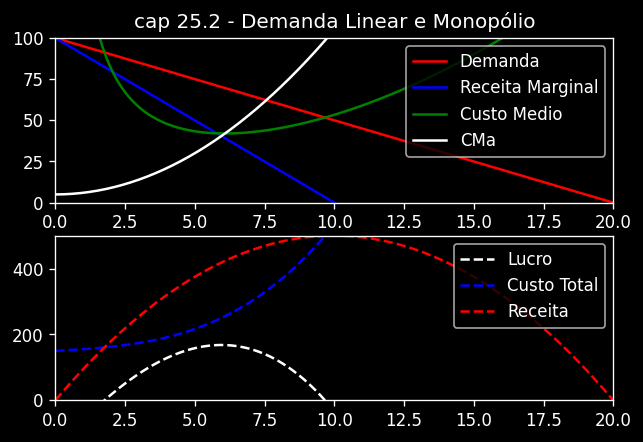
\includegraphics[scale=0.8]{cap25_2-demanda_linear_e_monopolio.png}
\end{center}

Para poder fazer essa simulação, eu tive de definir uma função custo e, consequentemente, uma função custo marginal\footnote{Eu tentei pensar numa função que apresentasse um comportamento parecido com a imagem que vemos no livro.}. Conseguimos ver que a curva de lucro tem um ponto de máximo exatamente onde a curva da receita marginal encontra o custo marginal. Qualquer ponto diferente desse levaria a um nível de lucro menor.
\\
\\
Além disso, também é relevante o fato da curva de custo médio estar abaixo da curva de demanda\footnote{Tente justificar isso matematicamente e, depois, tente criar uma situação onde isso acontece.}. Se o ponto de produção cuja receita marginal é igual ao custo marginal tiver um custo médio superior a demanda, a empresa receberá menos do que os custo de produção.\footnote{Veremos isso daqui a pouco no ponto 25.6.}.

\section{Estabelecimento de Preços com Markup}

Já conseguimos aprimorar nosso modelo de escolha da firma para o caso do monopolista. Agora que tornamos a receita marginal endógena, podemos ver as condições de maximização do lucro quando a firma tem poder de definir o preço ou a quantidade do mercado (mas não os dois ao mesmo tempo).
\\
\\
Podemos compreender essa última equação como uma política de preço do monopolista. Para isso, só precisamos isolar o termo $p(y)$ via rearranjo da última equação, o que após feito nos dá a seguinte relação

$$ p(y) = \frac{CMa(y)}{1 - 1/|\epsilon(y)|} $$
\\
Essa equação nos diz que o preço praticado no mercado cujo monopolista atua sempre\footnote{Sempre que ele agir de acordo com os pressupostos do nosso modelo de escolha.} se comportará como uma função de \textit{markup} do seu custo marginal. Podemos simplificar a visualização disso do seguinte modo

$$ p(y) = \phi \times CMa(y) $$
onde $\phi = \frac{1}{1 - 1/|\epsilon(y)|}$
\\
\\
Como sabemos, o monopolista sempre operará nos pontos cuja demanda é elástica, isso nos dará um $\epsilon(y) > 1$. Isso nos diz que o divisor $(1 - 1/|\epsilon|) <  1$, o que por sua vez, nos diz que $\phi > 1$.
\\
\\
Agora vamos dar uma olhada em um caso muito interessante: quando a curva de demanda possui a mesma elasticidade em todos os seus pontos.

\subsection{Demanda com Elasticidade Constante e Monopólio}

Para simular o caso da demanda com elasticidade constante, vamos usar o método do markup para encontrar o ponto de oferta do monopolista. Como esperado, teremos uma função de marcação acima da curva de custo marginal.

\begin{center}
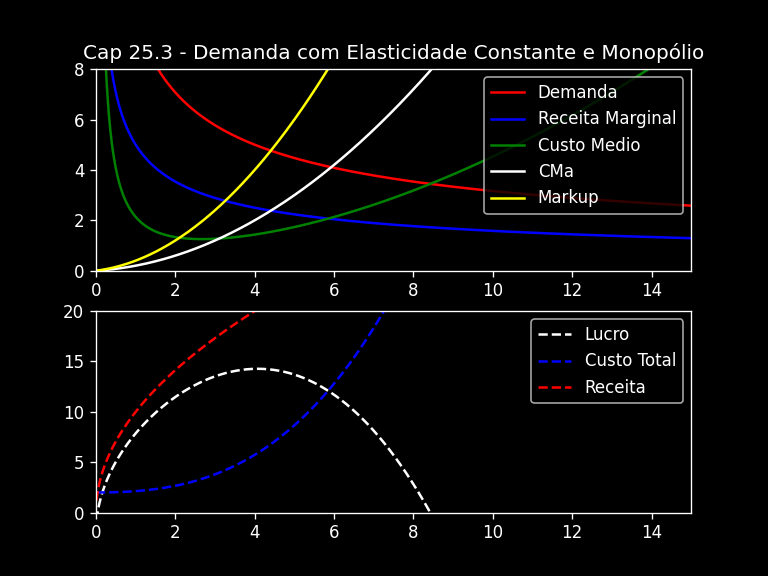
\includegraphics[scale=0.7]{cap25_3-demanda_ces_e_monopolio.png}
\end{center}

\textbf{Simulação:} \href{https://colab.research.google.com/drive/1MRJb9DZ7n_Hz2Kp9ng8K7pOcb1DTy_u5?usp=sharing}{Clique aqui} para ter acesso a essa simulação.
\\
\\
\textbf{Comentário:} Leia o exemplo sobre o impacto dos impostos sobre o monopolista na página 634. Com os conceitos vistos até agora, não deve ser difícil compreende-lo. Você pode acessar a simulação e modificar o custo variável para ver se o resultado é igual ao que você esperava.

\section{A Ineficiência do Monopólio}

Já conseguimos ver que, quando uma empresa opera como um monopólio, o preço de mercado será definido sempre acima do seu custo marginal. No mercado de competição perfeita, esse preço seria exatamente igual ao custo marginal. Isso implica na redução de algum excedente dos consumidores, mas em um incremento no excedente do produtor.
\\
\\
Como já sabemos, um arranjo é eficiente no sentido de Pareto se, e somente se, é possível realizar alguma troca de modo a se ter um aumento no excedente de uma das partes sem a redução do excedente de outra parte. Agora vamos investigar se o equilíbrio no mercado monopolista é eficiente. Considere a imagem abaixo.

\begin{center}
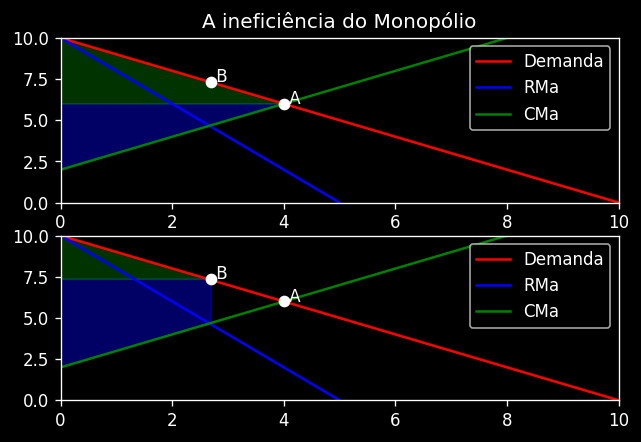
\includegraphics[scale=0.8]{cap25_4-inef_monopolio.png}
\end{center}

O gráfico da parte de cima é o equilíbrio no mercado de competição e o de baixo é o nosso equilíbrio com monopólio. Perceba como há um incremento no excedente do produtor (medido pela área azul) e uma redução do excedente do consumidor (área verde).
\\
\\
Para investigarmos se há uma ineficiência no sentido de Pareto no ponto $B$, façamos a seguinte pergunta: É possível adicionar uma unidade de produto no mercado de modo que o custo marginal pela produção desse bem seja inferior ao preço do mesmo? A resposta é claramente sim!
\\
\\
No nível $B$, a curva de preço (medida pela demanda inversa) ainda é superior à curva de custo marginal (aquela reta verde). Desse modo, se o monopolista produzisse mais uma unidade, ele receberia mais do que o custo marginal dessa unidade e os consumidores cujo preço de reserva é igual ao novo nível de preço passariam a consumir o produto. O excedente desse novo consumidor é igual a $0$, contudo, todos os que já consumiam o produto passaram a pagar menos do que antes o que aumentará os seus respectivos excedentes. Como o produtor teria um lucro positivo (pois o custo marginal é inferior ao preço) e os consumidores teriam um aumento de excedente, achamos uma melhoria de Pareto.
\\
\\
A razão para o monopolista abrir mão dessa receita adicional é devida a necessidade dele de ter que manter o mesmo preço para todos os compradores\footnote{Vamos explorar mais essa ideia no próximo capítulo.}. Diferente da empresa na competição perfeita, ele leva em consideração o impacto dessa unidade adicional no lucro. Essa redução do lucro se dá porque ao produzir mais, o preço de todas as unidades cai. Se ele pudesse manter o preço nas unidades anteriores e vender mais barato as novas, ele venderia. 

\section{O Ônus do Monopólio}

Agora que já vimos que o monopólio é ineficiente, podemos querer mensurar o tamanho dessa ineficiência. Uma maneira possível de medir essa ineficiência é observando os excedentes nos cenários competitivo e de monopólio. Observe a figura abaixo:

\begin{center}
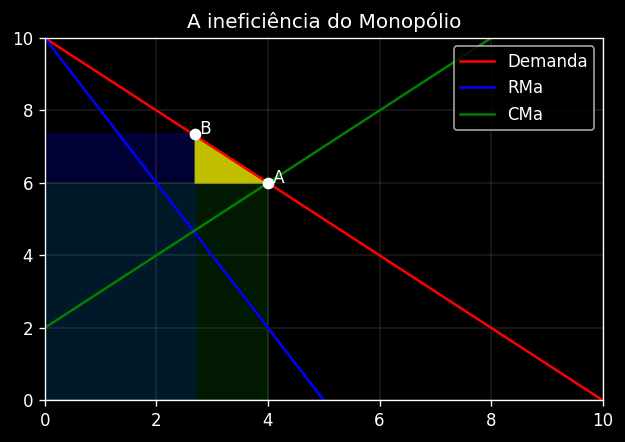
\includegraphics[scale=0.8]{cap25_5-onus_monopolio.png}
\end{center}

A área amarela é a medida da redução do excedente do consumidor. Em vermelho temos a redução do excedente do produtor. Em branco temos o quanto o monopolista consegue "capturar"\ do excedente dos consumidores ao adotar o nível de produção que maximiza o seu lucro.
\\
\\
A área branca não é definida como parte da ineficiência porque ela apenas demonstra uma transferência de excedente dos consumidores para o produtor. O \textbf{ônus resultante do monopólio} é precisamente a soma das áreas amarela e vermelha.
\\
\\
\textbf{Comentário:} Aqui o professor discorre sobre 3 exemplos do ônus do monopólio. Eu vou dar um resumo mas indico que você leia essa parte do livro.
\\
\\
No exemplo 1, vemos os casos das patentes (que, na prática, podem ser entendidas como um monopólio temporário). A ideia das patentes é criar um incentivo ao investimento em pesquisa e desenvolvimento de novas tecnologias. Contudo, por se tratar de um monopólio, acaba por criar um ônus atrelado a ele. O trabalho do Nobel William Nordhaus, demonstra que a estimativa da eficiência das patentes americanas é de 90\%, isso quer dizer que os consumidores estariam perdendo aproximadamente 10\% do seu excedente. O que parece indicar que o sistema de patentes não tem causado grandes malefícios.
\\
\\
No exemplo 2, ainda analisamos o mercado de patentes. Vemos que as patentes possuem 3 critérios de classificação: tempo de duração, extensão da proteção e novidade da invenção. Sendo os últimos dois muito subjetivos . Também discorremos sobre como o mercado de patentes permite algumas distorções (como o emaranhamento de patentes) de modo a tornar obrigatório para as empresas muito grandes a busca por grandes quantidades de patentes afim de se proteger de eventuais processos judiciais.
\\
\\
No exemplo 3, vemos o caso da isenção às proibições de \textit{antitrust} que os produtores agrícolas possuem nos EUA. Isso levou a uma pressão por parte dos grupos organizados dos produtores de batata a forçarem uma redução na quantidade ofertada do produto na ordem de 6,8 milhões de sacas. O que seria equivalente a 1,3 bilhão de pedidos de batata frita.

\section{Monopólio Natural}

Pois bem, já aprendemos o modelo de decisão do monopolista e também já vimos a ineficiência que esse modelo acarreta para os mercados. Ao percebemos que o monopólio produz aquém da quantidade ótima, poderíamos nos sentir tentados a propor regulações que obrigassem o monopolista a aumentar o seu nível de produção até o nível da competição perfeita. Contudo, esse problema é mais complexo do que parece, porque essa proposta de solução não leva em consideração a estrutura de custos.
\\
\\
Você mesmo pode fazer esse experimento, abra a simulação 25.2 ou a 25.3 e altere apenas o parâmetro "CF"\ que quer dizer "Custo Fixo". A medida que você aumenta esse parâmetro a curva de custo médio vai "subindo"\ e, em todos os pontos onde ele for superior a demanda, o monopolista terá lucro negativo.
\\
\\
Eu fiz 3 simulações para o caso da demanda com elasticidade constante. Uma com um custo fixo baixo, outra com um custo um pouco mais elevado e última com 10 vezes o custo fixo da primeira. Perceba ma imagem abaixo como a curva de lucro (da parte de baixo de cada painel vai caindo até desaparecer.

\begin{center}
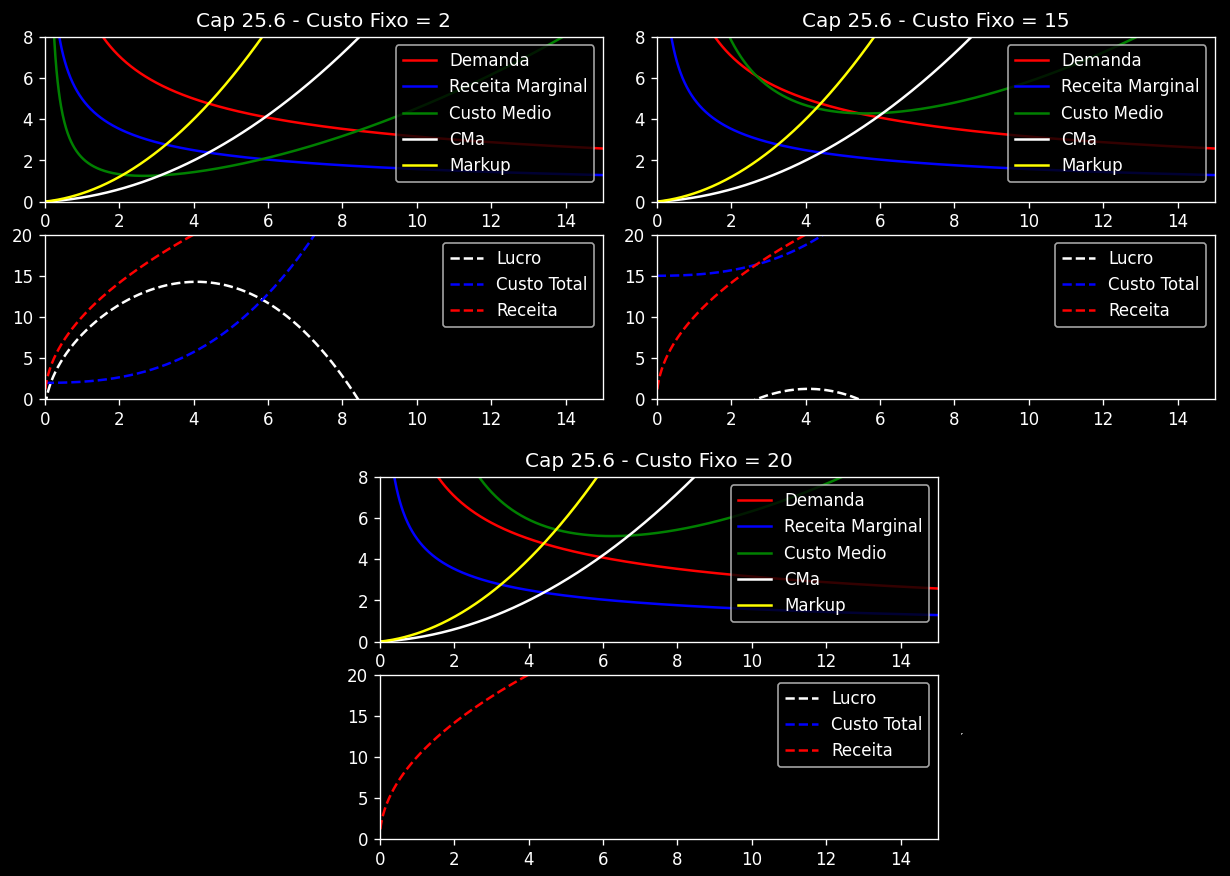
\includegraphics[scale=0.38]{cap25_6-monopolio_natural.png}
\end{center}

Chamamos de \textbf{monopólio natural} a situação onde temos uma estrutura de custo fixos muito alta e custos marginais baixos. Agora podemos ver que se obrigarmos o monopolista a produzir o nível da competição perfeita, pode acontecer do projeto não ser sustentável, pois a curva de custo médio está acima da curva de demanda.
\\
\\
Agora o dilema ficou um pouco mais complexo. Se forçarmos o monopolista a produzir a quantidade que iguala o custo marginal ao preço, ele terá prejuízo. Se aceitarmos que ele mesmo defina a quantidade a produzir, agirá num ponto que produzirá uma ineficiência no mercado.
\\
\\
Não existe solução simples para essa questão. Na maioria das situações os monopólios naturais são regulamentados ou operados diretamente pelos governos. Cada opção de solução acaba acarretando benefícios e malefícios consigo. Em ambos os casos, os problemas são geralmente oriundos devido a informação assimétrica entre a empresa e os seus controladores.

\section{O Que Causa os Monopólios?}

Parabéns, querido aluno. Agora você já compreendeu como um monopolista age, o que o comportamento dele acarreta no mercado e como o controle sobre o monopólio é mais complexo do que se parece a primeira vista. Agora nos resta uma última investigação: Qual a causa dos monopólios?
\\
\\
Uma variável que podemos creditar como importante é a \textbf{escala mínima de eficiêntia (EME)}. Ela nada mais é do que o ponto de mínimo da nossa curva de custo médio.\footnote{Podemos achar esse ponto pela derivada primeira da função custo médio igual a zero e pela derivada segunda menor igual a zero.} O formato da curva de custo médio (e consequentemente a EME) é definido exclusivamente pela tecnologia.
\\
\\
Quando temos uma escala mínima de eficiência muito elevada, uma empresa precisa produzir uma quantidade muito grande dos bens vendidos no mercado para se manter. A economia é advinda da economia de escala. O que implica em uma capacidade produtiva de porte elevado. Nesses mercados, a chance maior é que hajam poucos ofertantes, e consequentemente, que esses ofertantes acabem usufruindo do poder de mercado advindo da pouca competitividade.
\\
\\
Quando temos uma EME pequena, qualquer empresa pequena pode começar a operar no mercado. Isso aumenta o número de competidores. O que acaba por reduzir o peso de cada empresa individualmente. O que acaba por gerar um ambiente de competição.
\\
\\
Observe que o fator importante é a relação entre a EME e o tamanho do mercado. É possível que a quantidade de eficiência aconteça em 10.000 de unidades, mas se o mercado for o Brasil inteiro, ainda pode ser que hajam muitos ofertantes. Quando não é possível aumentar o tamanho do mercado e a EME é elevada, aí sim, nos deparamos com uma condição de monopólio que pode necessitar de regulação ou mesmo intervenção do Estado.
\\
\\
Além da EME, outra maneira de se criar um monopólio é por meio da coordenação dos agentes ofertantes em uma \textbf{colusão}\footnote{Um ajuste secreto entre ofertantes para prejudicar outras pessoas.}. Quando um conjunto de empresa se une para definir em conjunto a produção, elas agem como um \textbf{cartel}. Esse cartel acaba atuando como se fosse um ofertante só (e consequentemente, age com o poder de mercado advindo dessa coordenação).
\\
\\
Um terceiro e último motivo para o nascimento de um monopólio é o bom e velho "cheguei primeiro". Se uma empresa, por algum acidente histórico, é a primeira a se estabelecer no mercado. É natural que ela se valha da falta de competidores e consiga um crescimento em escala. Quando novos ofertantes entram no mercado, o monopolista consegue usar seu arsenal de escala e reduzir artificialmente o preço até o ponto onde ninguém além dele pode se manter.
\\
\\
\textbf{Comentário:} Aqui o professor cita alguns exemplo. Mesma coisa de antes, indico ler o livro porque eu só vou dar uma resumida aqui.
\\
\\
No exemplo 1, vemos ocaso do mercado de diamantes e a sua gigante participante De Beers. É um exemplo de monopólio por tamanho da participação no mercado.
\\
\\
No exemplo 2, temos um caso de poder de mercado advindo da cooperação de comerciantes de móveis antigos.
\\
\\
No exemplo 3, outro exemplo de conluio por parte dos ofertantes para fixação dos preços de microchips de memória RAM.

%%%%%%%%%%%%%%%%%%%%%%%% CHAPTER %%%%%%%%%%%%%%%%%%%%%%%%
\chapter{O Comportamento do Monipolista}

\begin{chapquote}{The Godfather}
	``Great men are not born great, they grow great \dots''
\end{chapquote}

Na prática, a maioria das empresas possui algum poder de mercado. É bem possível que um mercadinho eleve um pouco seus preços sem que isso acarrete a perda de todos os seus clientes. Nesse capítulo vamos ver quais estratégias as empresas podem adotar para aumentar e explorar o seu poder de mercado.
\\
\\
A medida que você vai avançando no seu curso de Microeconomia, o seu arcabouço de conhecimento vai ficando cada vez mais refinado e, consequentemente, próximo da realidade. Os modelos puros de competição perfeita e monopólio até existem, mas são mais raros na realidade quando comparados à competição monopolística.\footnote{Veremos mais sobre isso nesse capítulo.}

\section{Tipos de Discriminação de Preços}

No capítulo anterior, nós vimos que o monopolista acaba produzindo em um ponto onde a demanda ainda está disposta a pagar por mais do que o custo marginal. Vimos que a explicação do porquê ele não produz mais é que ele teria de baixar o preço de todos os produtos e não apenas os adicionais. Pois bem, existem alguns monopolistas que detém o poder de \textbf{discriminação de preços}. O professor classifica esse poder em 3 categorias:

\begin{itemize}
\item Discriminação de Preços de 1º Grau:
	\begin{itemize}
	\item[] Nesse caso ele tem poder de cobrar um preço diferente para cada consumidor e para cada quantidade.
	\end{itemize}
\item Discriminação de Preços de 2º Grau
	\begin{itemize}
	\item[] Nesse caso ele tem poder de discriminar o preço apenas para as quantidades compradas. Mas todos os consumidores que levarem a mesma quantidade, pagarão o mesmo preço no total.
	\end{itemize}
\item Discriminação de Preços de 3º Grau
	\begin{itemize}
	\item[] Esse é o caso mais comum. É quando o monopolista tem o poder de escolher qual preço cada pessoa vai pagar por todas as unidades que levar. Ou seja, ele pode controlar qual o valor de todas as unidades da cesta, contudo, não pode diferenciar o valor entre essas unidades.
	\end{itemize}
\end{itemize}

\section{Discriminação de Preços de 1º Grau}

Nesse caso, o monopolista está em \href{https://www.encurtador.com.br/eqCN1}{plenos poderes}. Ele possui conhecimento do preço de reserva\footnote{Lembra desse conceito?} de cada consumidor e, com esse conhecimento, cobra exatamente o valor máximo para cada quantidade. Também chamamos esse tipo de \textbf{discriminação perfeita}.
\\
\\
Um fato curioso desse arranjo é que, por incrível que pareça, ele é eficiente no sentido de Pareto. Uma vez que, para cada produto vendido, os consumidores pagam exatamente o valor máximo que estão dispostos a pagar, e consequentemente, o monopolista vai vender para todos os consumidores que tenham um preço de reserva maior ou igual ao custo marginal. O ponto final da produção será o ponto onde a quantidade iguala o custo marginal à curva de demanda.
\\
\\
Em termos de excedente, o que acontece é que o monopolista captura todo o excedente do mercado. Os consumidores, por sua vez, não possuem nenhum excedente.

\begin{figure}[H]
\centering
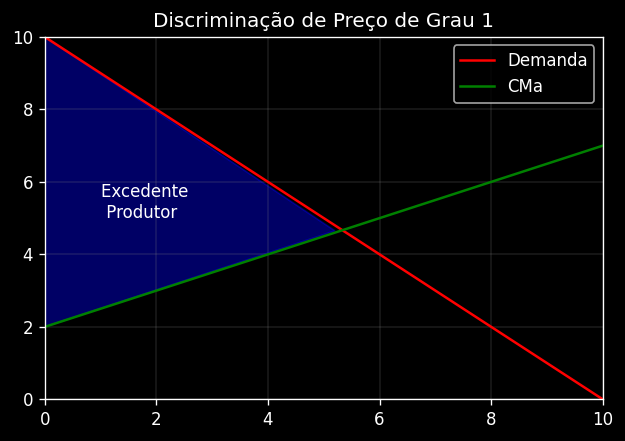
\includegraphics[scale=0.6]{cap26_2-discriminacao_grau1.png}
\end{figure}

Uma maneira conveniente se se pensar nessa situação é pela ótica da produção. Ao invés de pensar que o produtor olha para cada cliente e consegue cobrar exatamente o máximo que ele quer pagar, ele simplesmente oferta no mercado uma quantidade e deixa que os clientes definam quanto pagarão por ela. Claro que estamos supondo uma simplificação do comportamento das pessoas, mas a ilustração é válida.
\\
\\
O professor cita um exemplo da companhia aérea chamada Southwest Airlines. Que usou um software chamado Ding que faz ofertas periódicas e exclusivas para cada cliente cadastrado no sistema. Outro exemplo menos real, e mais icônico, é Mafioso Don Vito Corleone da clássica trilogia de filmes The Godfather (na abertura de todos os capítulos desse manual contém uma frase retirada dessa obra). O "modelo de negócio"\ do protagonista é fazer alguns favores em troca de outros favores. No caso do personagem mafioso, ele abusava do poder de mercado que detinha para cobrar o máximo possível (em bens ou serviços) de quem estava em dívida com ele.
\\
\ 
\\
\begin{figure}[H]
\centering
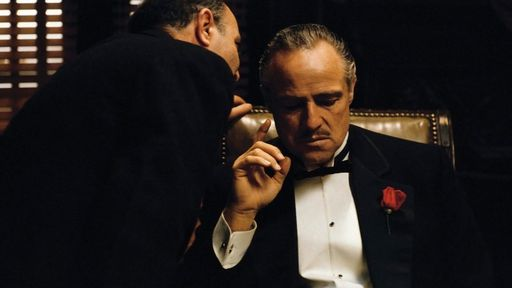
\includegraphics[scale=0.5]{cap26_2-don_corleone.jpeg}
\caption*{The Godfather (1972) - Paramount Films}
\end{figure}

\section{Discriminação de Preços de 2º Grau}

Nesse modelo, também chamado de \textbf{fixação de preços não linear}, o produtor já não pode cobrar, por uma mesma quantidade, um valor diferente entre consumidores diferentes. Isso força o monopolista a desenvolver uma estratégia de precificação que tente tirar o maior proveito possível das diferentes curvas de demanda.
\\
\\
\textbf{Comentário:} Eu não sei você, mas no meu caso, deu um trabalhão para entender o que o professor quis dizer nessa parte. Eu acho que o que deixou mais confuso foi ele ter suposto que o custo marginal é igual a zero (porque isso implicaria em dizer que ele venderia alguma cesta ao preço zero). Então eu retirei essa simplificação e reconstruí a mesma argumentação dele só que para um custo marginal constante maior que zero.\footnote{\href{https://www.youtube.com/watch?v=OBgziVdHH8w}{Esse vídeo aqui me ajudou bastante a entender melhor o que o professor quis dizer.}}
\\
\\
Imagine que temos apenas 2 grupos de consumidores no mercado. Como nosso modelo prevê, o monopolista tem acesso as curvas de demanda de cada consumidor, mas como limitação, ele só pode escolher quais cestas ofertar por qual preço, e deixar que os consumidores escolham qual é a melhor para eles. Chamamos esse modelo de \textbf{autosseleção}.
\\
\\
O objetivo do monopolista é captar todo o excedente do mercado. Mas ele enfrenta uma limitação nessa modalidade de discriminação de preços. Como ele não pode vender a mesma quantidade a preços diferentes para os grupos de consumidores, ele tem de escolher se vai vender a preço de reserva da curva de demanda 1 ou 2.

\begin{figure}[H]
\centering
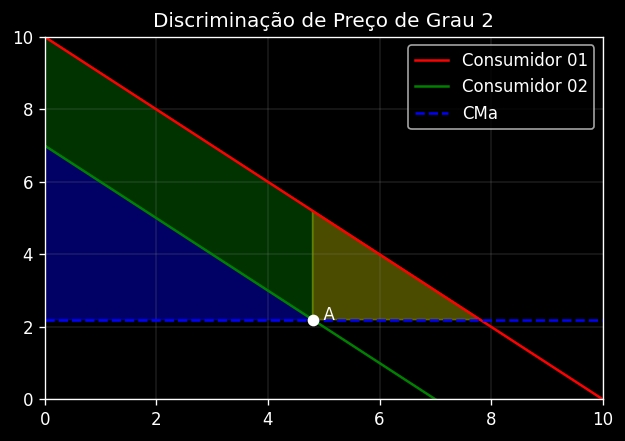
\includegraphics[scale=0.8]{cap26_3-discriminacao_grau2_1.png}
\end{figure}

Se ele optar por vender na fronteira da curva de demanda 1, ele vai abrir mão de todo o excedente advindo dos consumidores do tipo 2! Isso significaria abrir mão do toda a área azul na figura acima. Como ele não vai fazer isso, ele adotará a seguinte abordagem: Vender de $0$ até o ponto $A$ pelo preço de reserva da curva de demanda dos consumidores do tipo 2 e, a partir desse ponto, vender pela fronteira do preço de reserva dos consumidores do tipo 1. Isso garantirá que ele obtenha todo o excedente da área azul e também da área amarela.
\\
\\
Não satisfeito, o monopolista pode pensar um pouco mais e perceber que ele pode escolher uma opção que aumentará o seu excedente. Veja o que acontece se ele decide optar pela fronteira do consumidor tipo para uma cesta cuja quantidade é um pouco menor que a cesta $A$.

\begin{figure}[H]
\centering
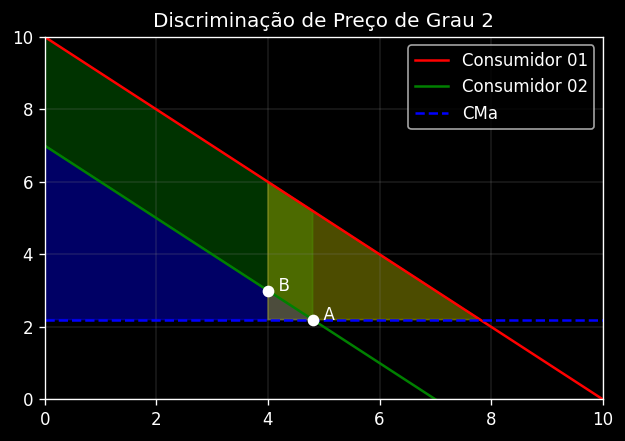
\includegraphics[scale=0.8]{cap26_3-discriminacao_grau2_2.png}
\end{figure}

Veja só que interessante, como no ponto $B$ o preço não é igual ao custo marginal para o consumidor tipo 2, haverá uma perda no total do excedente capturado pelo monopolista, mas em contrapartida, veja como a área amarela aumentou muito mais do que a área de perda do excedente do primeiro grupo. Isso quer dizer que, ao aumentar o preço da cesta, optando por adotar o preço de reserva do consumidor tipo 1 em um ponto anterior ao custo marginal igual à demanda tipo 2, o monopolista "abre mão"\ de uma pequena parte do excedente tipo 1 e ganha uma grande parte do excedente tipo 2. Não é difícil prever que ele continuará reduzindo a quantidade até o ponto onde o excedente perdido de um grupo é igual ao excedente ganho do outro.

\begin{figure}[H]
\centering
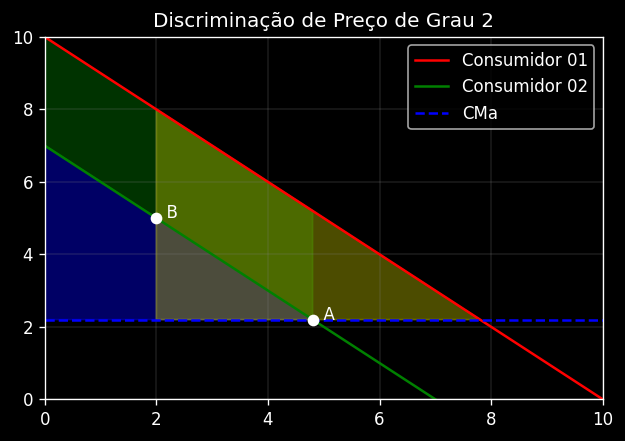
\includegraphics[scale=0.8]{cap26_3-discriminacao_grau2_3.png}
\end{figure}

A partir desse novo ponto $B$, o excedente perdido dos consumidores tipo 2 com o aumento do preço da cesta é maior que o ganho adicional do excedente dos consumidores tipo 1. Desse modo o monopolista acaba com um excedente total igual à área azul e toda a área amarela.
\\
\\
\textbf{Comentário:} Alguns de vocês podem pensar que o excedente abaixo da curva de demanda verde foi inteiramente perdido. Mas não é o caso! Perceba que, mesmo com a retirada dos consumidores do tipo $2$, essa área de excedente foi preenchida pelo excedente dos consumidores do tipo $1$. O monopolista abre mão no sentido que antes essa área era computada duas vezes (uma vez para cada tipo de consumidor).
\\
\\
Na realidade, o principal método de incentivo a autosseleção é a alteração da qualidade do bem. Normalmente, o monopolista reduz a qualidade dos produtos direcionados aos consumidores com preços de reserva menores, afim de evitar que seus consumidores dispostos a pagar mais, prefiram comprar esses produtos ao invés de produtos de "primeira linha". Essa estratégia maximiza o lucro do monopolista e ainda garante algum excedente para os consumidores das demandas mais altas.
\\
\\
O professor coloca dois exemplos que são espetaculares. Um sobre a diferença nos preços das passagens aéreas e o motivo da existência das classes econômica e executiva nos meios de transporte. Recomendo demais a leitura. O segundo é referente ao mercado de remédios.

\section{Discriminação de Preços de 3º Grau}

Só nos resta o último tipo de discriminação de preços. Nesse caso, o monopolista consegue discernir claramente qual consumidor pertence a qual grupo e, consequentemente, consegue cobrar um preço diferente. Atente para o fato que o monopolista só pode adota um único preço para cada grupo de consumidores.
\\
\\
Na prática, a modelagem desse problema é muito parecida com o que vimos no capítulo passado, já que, ele só pode escolher um único preço para cada tipo de consumidor. A única diferença do modelo do capítulo passado é que ele vai se deparar com mais de uma curva de demanda. Veja a formalização do problema logo abaixo

\begin{center}
\LARGE $\stackrel{máx}{\text{\small $y_1,y_2$}} \ \ \stackrel{p_1(y_1)y_1 + p_2(y_2)y_2 - c(y_1 + y_2)}{\ }$ \\
\end{center}

Esse problema nada mais é do que uma adaptação do problema da maximização da receita. Veja que $p_1(y_1)y_1$ nada mais é do que a receita obtida com a venda do produto para o grupo 1. Desse modo, o problema de maximização é a receita total obtida (que é a soma das receitas da venda para cada grupo) menos o custo total de produção.
\\
\\
Da mesma maneira de antes, a otimização será dada por:

$$ RM_1(y_1) = CMa(y_1+y_2) $$
$$ RM_2(y_2) = CMa(y_1+y_2) $$

Isso claramente implica em

$$ RM_1(y_1) = RM_2(y_2) = CMa(y_1+y_2) $$

\textbf{Atenção:} Eu acho que encontrei um erro de tradução no parágrafo que vem logo depois dessa expressão das receitas marginais acima. Na tradução, temos o trecho: "se a receita marginal no mercado 1 ultrapassar o custo marginal, valeria a pena aumentar a produção \textbf{nos dois mercados}". Isso está errado! No original temos a seguinte passagem: "if the marginal revenue in market 1 exceeded marginal cost, it would pay to expand output \textbf{in market 1}, and similarly for market 2". Uma tradução melhor seria algo como: "se a receita marginal no mercado 1 for maior que a o custo marginal, então valerá a pena aumentar a produção no mercado 1, a mesma lógica se aplica ao mercado 2".
\\
\\
Podemos usar a nossa fórmula da elasticidade para elaborar um pouco mais esse problema:

$$ p_1(y_1) \left[1 - \frac{1}{|\epsilon_1(y_1)|} \right] = CMa(y_1 + y_2) $$
$$ p_2(y_2) \left[1 - \frac{1}{|\epsilon_2(y_2)|} \right] = CMa(y_1 + y_2) $$
\\
Suponha que $y_1 = y_2$. Se $p_1 > p_2$, então:

$$ 1 - \frac{1}{|\epsilon_1(y_1)|} < 1 - \frac{1}{|\epsilon_2(y_2)|} $$
\\
O que implica em

$$ \frac{1}{|\epsilon_1(y_1)|} > \frac{1}{|\epsilon_2(y_2)|} $$
\\
Que, por fim, nos diz que

$$ |\epsilon_1(y_1)| < |\epsilon_2(y_2)| $$
\\
Não continue lendo se você não entendeu essa afirmação. Pare e pense até sentir que compreendeu o argumento. Se ainda tiver dúvida \href{https://twitter.com/bruno_ruas2}{me manda um twite que eu te ajudo}.
\\
\\
Dessa maneira, podemos ver que quanto mais elástico for o mercado, menor será o seu preço. Faz todo sentido porquê quanto mais elástica é a demanda, mais sensível ela será às alterações de preços. Portanto, o monopolista vai conseguir elevar o preço sempre que a demanda for inelástica e manterá o preço comparativamente mais baixo nos grupos de demanda mais elástica. Isso maximizará o seu lucro em cada grupo de consumidores.
\\
\\
\textbf{Comentário:} Querido aluno, agora você tem todo o arcabouço teórico necessário para entender o motivo de você pagar meia entrada no cinema\footnote{Entender isso é muito top, fala sério.}. Os cinemas acreditam que uma elevação dos preços levaria vocês a buscar outros serviços além do cinema, visto que é comum supor que essa fase da vida tenha restrição orçamentária consideravelmente modesta. Por outro lado, um executivo de uma empresa tem um preço de reserva muito maior que o de vocês, então o cinema cobra dele mais caro para entrar (sem falar o preço "salgado"\ das pipocas).
\\
\\
Agora o professor coloca três exemplos. O primeiro é teórico, o segundo é um exemplo de aplicação e o terceiro é uma aplicação do conceito ao mercado de revistas acadêmicas. Eu vou criar uma simulação do segundo exemplo.

\subsection{Curvas de Demanda Lineares}

O monopolista precisa lidar com duas curvas de demanda (que suporemos serem lineares) do tipo:

$$ D_1(p_1) = 100 - p_1 $$
$$ D_2(p_2) = 100 - 2p_2 $$
\\
As demandas inversas dessas funções são

$$ p_1(y_1) = 100 - y_1 $$
$$ p_2(y_2) = 50 - y_2/2 $$
\\
As funções de receita serão iguais a

$$ r_1(y_1) = 100y_1 - y_{1}^{2} $$
$$ r_2(y_2) = 50y_2 - \frac{y_{2}^{2}}{2} $$
\\
Cujas receitas marginais serão

$$ RMa_1(y_1) = 100 - 2y_{1} $$
$$ RMa_2(y_2) = 50 - y_{2} $$
\\
Para simplificar vamos supor que o custo marginal é contante em $CMa = \$ 20,00 $. Com isso já podemos criar uma simulação do modelo. Mas antes de colocar o computador fazer isso, nós podemos encontrar os pontos de máximo facilmente ao igualar as funções de receita marginal ao custo marginal.

$$ 100 - 2y_{1} = 20 \hspace{100pt} 50 - y_{2} = 20 $$
$$ 100 - 20 = 2y_{1} \hspace{100pt} 50 - 20 = y_{2} $$
$$ 80/2 = y_{1} = 40 \hspace{120pt} y_2 = 30 $$
\\
Sabemos que os pontos de maximização do lucro para cada curva de demanda serão os pontos cujas quantidades são iguais a $y_1 = 40$ e $y_2 = 30$. Para descobrir os preços, basta colocar esses valores nas funções de demanda inversa. Podemos ver que esses são os pontos que estão no topo das curvas de lucro 1 e 2.

\begin{figure}[H]
\centering
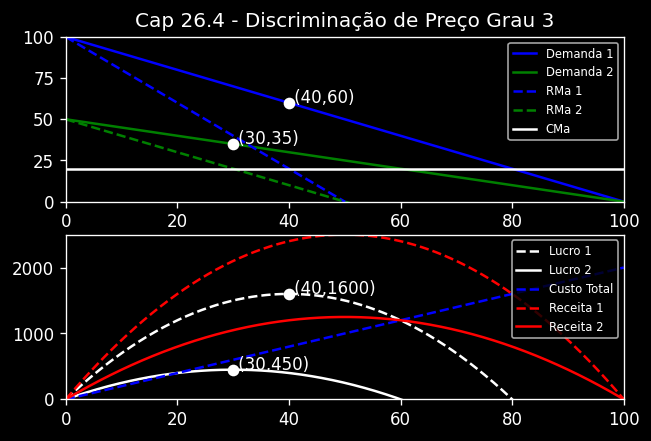
\includegraphics[scale=0.8]{cap26_4-discriminacao_grau3.png}
\end{figure}

\textbf{Simulação:} \href{https://colab.research.google.com/drive/1TYSpJLSEg4yInKX_viA6aP8qLiRsHdBm?usp=sharing}{Clique aqui} para ter acesso a essa simulação.
\\
\\
Se, por outro lado, o monopolista não puder fazer essa separação dos preços, teremos que somar as demandas como se fosse uma única e trabalhar a otimização como no primeiro modelo do capítulo 25.

\begin{figure}[H]
\centering
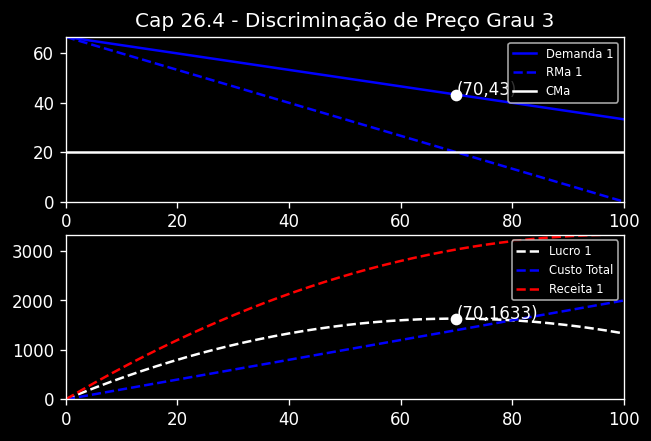
\includegraphics[scale=0.8]{cap26_4-discriminacao_grau3_2.png}
\end{figure}

\textbf{Atenção:} Quando trabalharmos com demandas somadas, temos que testar se o preço de equilíbrio não gera demanda negativa em alguma das curvas de demanda. Se a função demanda for negativa ao preço de equilíbrio, isso quer dizer que o monopolista aumentará o seu lucro se não vender para esse grupo de consumidores. Ao excluir essa demanda e calcular o novo equilíbrio, seu lucro aumentará.

\section{Vinculação de Produtos}

Uma prática muito comum entre as empresas é a \textbf{venda casada}. Você já se perguntou qual o motivo das empresas de internet se esforçarem tanto para vender o pacote TV + Internet + Telefone?. Pois bem, agora você vai ter uma ideia por trás dessa estratégia.\footnote{Aqui estamos supondo que as demandas por esses serviços não são relacionadas. Mas não leve esse primeiro parágrafo tão ao pé da letra. O objetivo dele é só vender o conteúdo do tópico ;)}
\\
\\
Já vimos que a vontade do monopolista é cobrar o máximo possível para cada cliente em cada quantidade. Isso faria com que ele capturasse todo o excedente do mercado. Como na prática isso implicaria em conhecimento perfeito de todos os consumidores e existe uma legislação que limita a capacidade de impor muito do poder de mercado, as empresas se valem de estratégias para maximizar esse excedente.
\\
\\
Uma dessas estratégias é exatamente a venda casada. A ideia é a seguinte: como o vendedor não pode cobrar um preço para cada consumidor, ele precisa ter uma ideia dos preços de reserva dos mesmos para que possa cobrar exatamente o valor do preço de reserva mais baixo que o custo marginal permita.
\\
\\
Veja a tabela 26.1 a página 672 do livro. Temos dois tipos consumidores que possuem preços de reservas inversos para dois tipos de programas diferentes. Se o monopolista cobrar $U\$ 101,00$ pelo processador de texto, ele perderá 100\% dos consumidores do tipo A. Por causa disso, ele sempre cobrará o mínimo possível para poder capturar o preço de reserva mais baixo. Isso implica que os consumidores que possuem preços de reserva maiores tenham algum excedente.
\\
\\
Mas como bem sabemos, as empresas sempre pensam em novas estratégias. No caso da vinculação de produtos, supondo que o preço de reserva pelos produtos juntos seja igual à soma dos preços individuais, nós tratamos os dois produtos como uma cesta única. Nesse novo arranjo, o vendedor consegue cobrar um preço maior, porque o preço de reserva por cesta é maior que o valor cobrado separadamente.
\\
\\
Eu expandi um pouco do exemplo do professor Varian para um caso de 1.000 consumidores. Nessa simulação os preços de reserva são aleatórios entre 51 e 100. Para cada uma das duas abordagens, eu comparei os lucros a medida que se eleva o preço praticado no mercado. Para efeito de simplificação, os preços de reserva mínimos são iguais nos dois produtos, então o vendedor sempre aumentará os preços em paralelo. Atente para o fato de que nesse gráfico o preço está no eixo horizontal.\footnote{Ficou na dúvida, fala comigo que eu explico melhor.}

\begin{figure}[H]
\centering
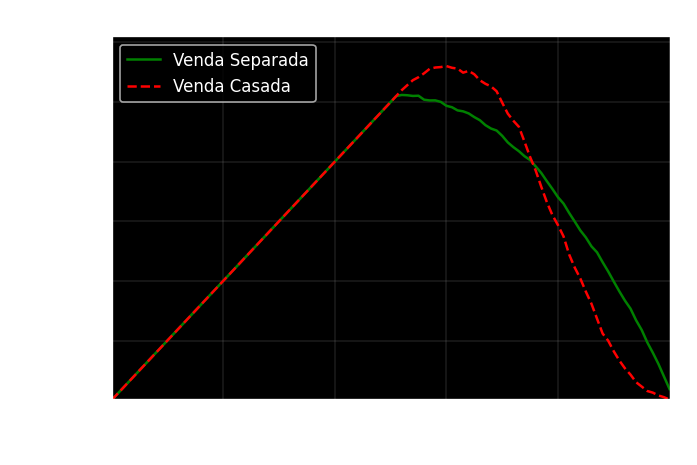
\includegraphics[scale=0.8]{cap26_5-venda_casada.png}
\end{figure}

\textbf{Simulação:} \href{https://drive.google.com/file/d/1WhxGaAhUB9dKkgrKWadihIrzS4cm3bXP/view?usp=sharing}{Clique aqui} para ter acesso a essa simulação.
\\
\\
De zero até 50, a curva de lucro é uma linha reta porque o preço de reserva mínimo da nossa simulação é 50. Então, sempre existirá alguém disposto a comprar a medida que ofertamos até esse preço. A partir desse ponto, cobrar mais caro implica em abrir mão dos consumidores com preço de reserva menor que o preço.

\section{Tarifas Bipartidas}

Um artigo famoso de 1971 cujo título é "A Disneyland Dilemma: Two-Part Tariffs for a Mickey Mouse Monopoly", de Walter Oi, nos mostra uma situação interessante. Como o monopolista se comportará no caso da venda de dois produtos que possuem demandas interrelacionadas?
\\
\\
No tópico anterior, supomos que as demandas eram independentes. Agora temos um caso onde, ao aumentar a oferta do bem 1, os consumidores estarão menos propensos a consumir o bem 2. Chamamos esse arranjo de \textbf{tarifa bipartida}.
\\
\\
Como já trabalhamos antes, sabemos que a maximização do lucro é obtida no ponto onde o custo marginal é igual à receita marginal. Fazendo isso para a oferta do bem 1 e como ele não pode discriminar perfeitamente os preços, haverá um excedente do consumidor. Esse excedente é exatamente o valor máximo que ele pode cobrar pelo bem 2. Nesse caso, pode ser que a quantidade cobrada pelo bem 2 seja inferior ao montante que iguale o custo marginal à receita marginal.
\\
\\
Para elucidar esse modelo eu fiz uma simulação. Fora suposto que as demandas são lineares, com a mesma forma funcional e interdependentes, ou seja, quanto mais de um bem se tem, menos do outro terá. Os custo marginais são fixos em 20.
\\
\\
Como esse problema envolve o equilíbrio em dois mercados (bem 1 e bem 2), eu optei por construir um gráfico tridimensional. O problema dessa abordagem é que a melhor maneira de se entender um gráfico desse é pela mudança do ângulo da câmera. Então eu vou colocar 3 perfis de visualização mas também fiz um gif com um panorama dos eixos \href{https://github.com/brunoruas2/Meus_Estudos/blob/main/Microeconomia/Microeconomics\%20-\%20Hal\%20Varian/images/cap26_6-tarifas_bipartidas.gif}{\textbf{clique aqui para ver}}.

\begin{figure}[H]
\centering
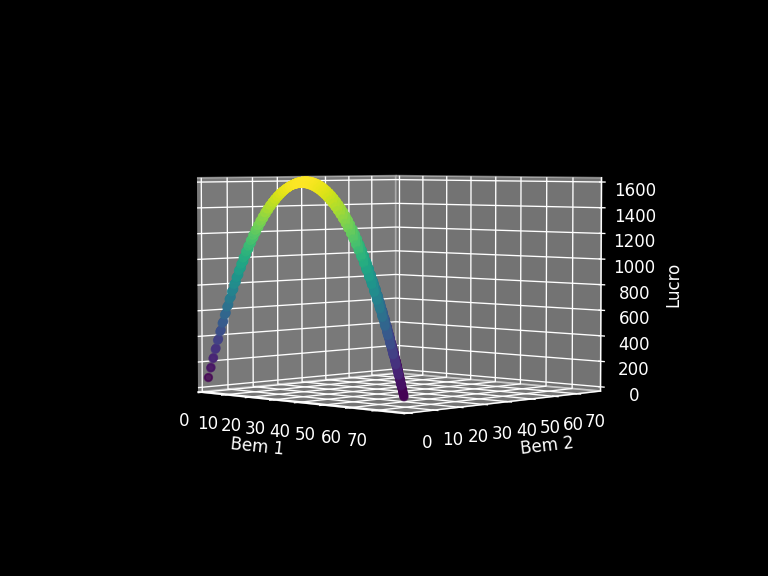
\includegraphics[scale=0.6]{cap26_6-tarifas_bipartidas1.png}
\end{figure}

Nessa primeira imagem temos um ângulo que evidencia como o lucro se comportaria se só existisse o mercado do bem 1. Podemos ver que o lucro é maximizado em um ponto (que é justamente onde o custo marginal é igual à receita marginal. A segunda imagem é similar a primeira, mas para o outro bem.

\begin{figure}[H]
\centering
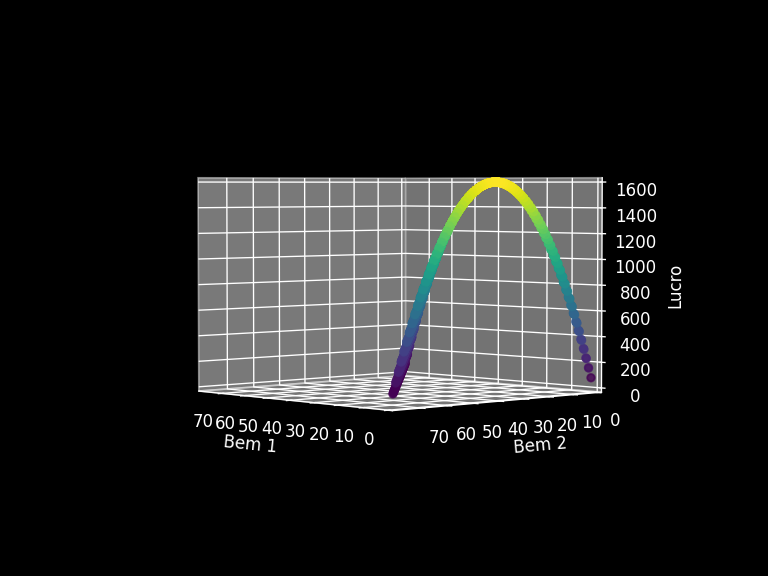
\includegraphics[scale=0.6]{cap26_6-tarifas_bipartidas2.png}
\end{figure}

A terceira mostra como o monopolista deverá agir para poder ofertar ambos os bens. O padrão é simétrico porque no modelo as duas demandas possuem as mesmas formas e os mesmos coeficientes. Veja como a figura do lucro forma um tipo de "onda"\ que parte da cesta onde os dois bens são iguais a zero. Na parte amarela temos o máximo do lucro possível para cada cesta. E, a partir desses pontos de máximo, os lucros de cada cesta vão sendo cada vez menores.

\begin{figure}[H]
\centering
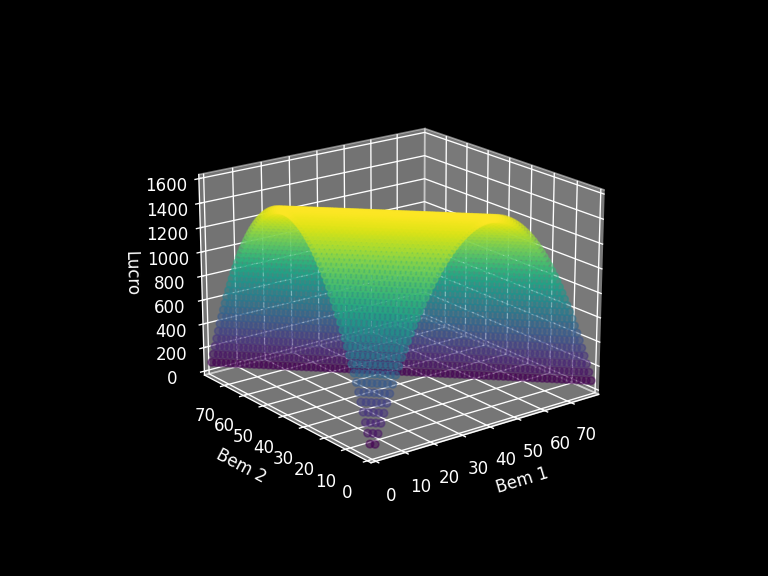
\includegraphics[scale=0.8]{cap26_6-tarifas_bipartidas3.png}
\end{figure}

A última mostra um ângulo onde vemos a relação de troca entre os bens (a linha vermelha indica a reta onde as cestas maximizam o lucro). Observe que, visto de cima, temos um gráfico que demonstra o quanto o monopolista tem que abrir mão de um bem para vender mais do outro, sem que isso incorra em redução do seu lucro total.\footnote{Pra mim, lembra um pouco a curva de restrição orçamentária do consumidor.}

\begin{figure}[H]
\centering
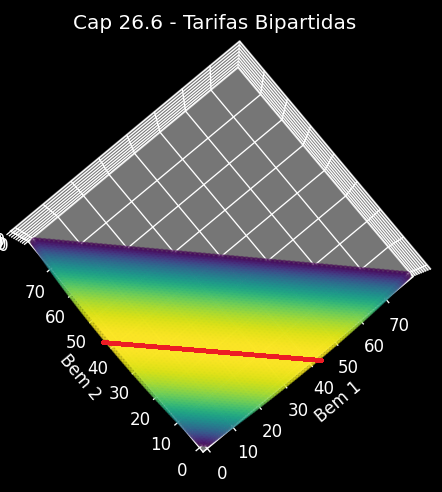
\includegraphics[scale=0.60]{cap26_6-tarifas_bipartidas4.png}
\end{figure}

Como as demandas desse modelo são simétricas e os custos são iguais, o modelo gráfico é uniforme. Na imagem abaixo eu simulei o mesmo modelo para o caso onde o custo marginal do bem 2 é igual a zero.

\begin{figure}[H]
\centering
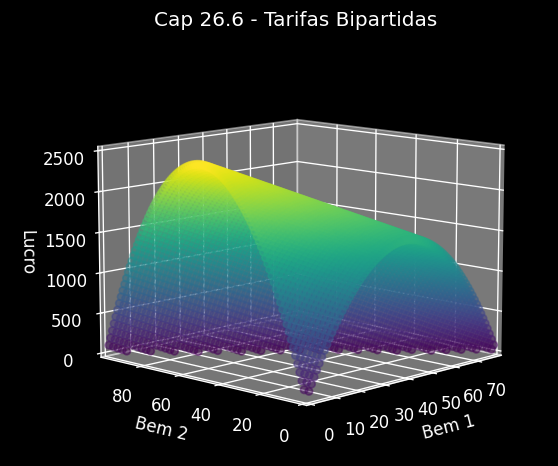
\includegraphics[scale=0.75]{cap26_6-tarifas_bipartidas5.png}
\end{figure}

Podemos ver claramente que, nesse segundo caso, o monopolista só maximiza seu lucro ao vender exclusivamente o bem 2.
\\
\\
Essa assimetria é a explicação do motivo da Disney não cobrar um preço pela entrada nos brinquedos, uma vez que em os custos dos serviços (a saber: a entrada e os passeios) não são iguais. A Disney percebeu que ao cobrar somente a entrada, poderia captar mais o excedente total do mercado do que se cobrasse também os passeios aos brinquedos.

\section{Competição Monopolística}

Nós começamos essa seção do livro partindo da posição oposta aos modelos que vimos ao longo da primeira metade do curso. Adaptamos o modelo da escolha maximizadora do lucro para a existência do poder de mercado e avançamos como o monopolista pode usar esse poder mesmo em arranjos menos favoráveis à capacidade de discriminação de preços. Nessas últimas duas seções expandimos nosso modelo para mais de um produto e como eles podem interagir entre si para a maximização do lucro.
\\
\\
Todo esse caminho foi muito bem pensado pelo professor. Lá no começo alguns de vocês podem ter achado a hipótese da existência de apenas um produtor um tanto quanto caricata. Mas agora vamos trazer o nosso modelo da escolha para mais perto da realidade presenciada todos os dias por vocês.
\\
\\
Até agora, tratamos uma \textbf{indústria} como um conjunto de produtores cujo resultado do esforço produtivo era \textit{exatamente} a mesma mercadoria. Isso quer dizer que, sendo 1 (que é o caso do monopólio) ou 1.000 produtores, todas as mercadorias que saem das fábricas e são comercializadas seriam exatamente as mesmas. Essa hipótese simplificadora vai dar lugar a uma nova que, na minha opinião, é bem mais aplicável a nossa realidade fática.
\\
\\
Os produtos agora possuem certas propriedades exclusivas (sendo a marca a principal) e seus competidores também serão diferenciáveis entre si. Todos competindo por um mercado de bens relativamente parecidos aos consumidores. Além disso, vamos considerar que a barreira de entrada de novos produtores também será mais baixa.
\\
\\
Nesse novo arranjo, os produtores possuem características de ambos os modelos vistos. Eles não podem alterar seus preços completamente como um monopólio, porque os consumidores olhariam para os seus concorrentes e comprariam algum produto semelhante ao seu, só que mais barato. Por outro lado, eles não estão fadados estritamente ao preço de mercado, uma vez que nesse arranjo a demanda não será infinitamente elástica. O nome dessa estrutura setorial é \textbf{concorrência monopolística}.\footnote{Eu não sei você, mas eu acho esse modelo muito empolgante de ser estudado.}
\\
\\
Estamos vendo apenas vantagens ao novo modelo, mas como tudo na vida, temos um trade-off entre realidade e praticidade. Esse modelo é bem mais complexo de ser construído e analisado. Como o próprio professor diz "Em um modelo detalhado do setor de competição monopolística, dependemos muito dos detalhes específicos dos produtos e da tecnologia (de produção), assim como da natureza das escolhas estratégicas disponíveis para as empresas". Isso acaba implicando naquela situação clássica de "cada caso é um caso". Por causa disso, e do fato desse curso ser introdutório, vamos apenas ver alguma das principais estratégias dos economistas para modelar esses mercados.
\\
\\
Mesmo sendo um modelo mais complexo, podemos evidenciar algumas características que independam de quaisquer fatores relacionados ao mercados específicos. O primeiro deles é relacionado ao número de competidores.
\\
\\
É razoável supor que se o número de concorrentes aumentar (algo que está muito relacionado às barreiras de entrada) haverá impactos na curva de demanda que a empresa está imposta. O primeiro impacto que podemos supor é que essa curva irá se aproximar mais da origem do plano cartesiano\footnote{Ou seja, ele vai acabar tendo que baixar mais o seu preço se quiser continuar vendendo a mesma quantidade.}. O segundo impacto previsto é que a elasticidade de demanda aumentará\footnote{Porque agora os consumidores podem escolher mais opções em relação a antes.}.
\\
\\
Se todas as empresas do mercado tiverem como objetivo o lucro. 
Qualquer equilíbrio alcançado terá que obedecer algumas restrições:
\begin{itemize}
\item Cada empresa venderá o máximo possível. Ou seja, elas sempre optam por ofertar cestas que estejam na curva de demanda e não abaixo dela.
\item Cada empresa precisará maximizar seu lucro levando em consideração as imposições oriundas à sua curva de demanda da empresa.
\item Quanto mais competidores o mercado tiver, mais próximo de zero será o lucro das empresas contidas no mercado.
\end{itemize}

Do fato 1, podemos derivar o fato que quaisquer opções de maximização estão na própria curva de demanda\footnote{Afinal, ela mostra as maiores quantidades para cada nível de preço.}. Do fato 3, podemos ver que a medida que o número de competidores tende ao infinito, a cesta escolhida deve ser num ponto onde a curva de custo médio tangencia a curva de demanda\footnote{A lógica é que se $p > c(y)/y$ então $py - c(y) > 0$, o que contraria nosso postulado. Agora, se $p = c(y)/y$ então, $py - c(y) = 0$, que é exatamente o que estamos dizendo.}. Por fim, o nosso postulado 2 afirma que a maximização ocorrerá na curva de demanda, isso implica no fato que a curva de custo médio não cruzará a curva de demanda, porque se isso acontecer, as empresas terão lucro positivos.
\\
\\
Existem algumas características desse equilíbrio competitivo monopolizador:
\begin{itemize}
\item Ele é ineficiente no sentido de Pareto, porque a maximização ocorre pelo custo médio e não pelo custo marginal. Mesmo sendo uma situação de lucro zero, quando tratamos de eficiência, estamos trabalhando com a maximização do excedente do mercado. E isso se dá pelo custo marginal.
\item As empresa acabam por atuar num ponto a esquerda do nível de produção. Isso quer dizer que os consumidores acabam não tendo acesso a todas as mercadores que os produtores realmente poderiam lançar no mercado.
\end{itemize}

Um fato interessante desse segundo ponto é que temos um trade-off interessante. Vimos que as empresas até teriam como ofertar quantidades maiores, mas como a maximização do lucro se dá pelo custo médio, elas não produzem tudo que podem. Se quiséssemos aumentar a oferta dos produtos, teríamos que reduzir a quantidade de ofertantes. Isso realmente aumentaria a quantidade ofertada por cada empresa, mas em contrapartida, os consumidores teriam menos opções para escolher!. Esse é o tipo de situação onde não existe regra de ouro e cada caso é único.

\section{Modelo de Diferenciação de Produtos por Local (Estabilidade na Competição)}

Esse seção é inspirada no clássico artigo de 1929 "Stability in Competition"\ de Harold Hotelling.\footnote{Imagina como deve ter sido doido publicar um artigo em 1929.}
\\
\\
Como foi dito antes, as abordagens puramente teóricas nessa parte da teoria microeconômica são limitadas porque agora os aspectos únicos de cada mercado acabam tornando praticamente impossível deduzirmos leis gerais. Na seção passada nós já aprendemos como um concorrente monopolista possui algumas restrições e alguma liberdade advinda da diferenciação dos produtos (que não é absoluta, mas existe). Agora, porém, vamos abordar outro tipo de diferenciação: A geográfica.
\\
\\
Nossos modelos sempre adotaram que os consumidores não possuíam nenhum custo pela aquisição além do preço. Mas, na realidade, todos nós precisamos sair de casa e perdermos um tempo indo até o local onde teremos acesso aos produtos que desejamos\footnote{Ou optamos por pagar a bendita taxa de entrega do Ifood afim de termos a comodidade de receber a comida na porta de casa.}.
\\
\\
Pensando nisso vamos criar um \href{https://en.wikipedia.org/wiki/Thought_experiment}{experimento mental}:
\\
Imagine que a orla da Ponta Negra seja retilínea e que só seja permitida a venda de sorvetes mediante autorização da Prefeitura. Adicionaremos a restrição que a probabilidade de você encontrar um transeunte com calor é uniforme em toda a extensão da orla. Suporemos também que os preços dos sorvetes sempre serão iguais, que não há diferença de qualidade e que por motivos climáticos só exista um único sabor disponível.
\\
\\
Diante das características do mercado acima, onde o primeiro sorveteiro com licença da prefeitura deve instalar sua barraquinha? Não é difícil chegar na conclusão que ele deve se instalar exatamente no meio da orla. Desse modo, a distância máxima que um transeuntes com calor terá de caminhar para aliviar seu desconforto térmico é de meia orla.
\\
\\
Agora vamos complicar um pouco mais. Supondo que outro sorveteiro consiga sua licença para vender na orla. Qual será o melhor arranjo? Se usarmos o mesmo pensamento de antes, podemos supor que cada vendedor fique no ponto que corresponda a 1/4 e 3/4 do tamanho da orla. Nesse caso, todos os consumidores das áreas 1/4 e 2/4 estariam próximos ao vendedor 1. E os consumidores dos setores 3/4 e 4/4 estariam mais próximos do sorveteiro 2. No final teremos uma distância máxima de 1/4 da orla para cada consumidor e 1/2 da receita total para cada sorveteiro.
\\
\\
Tudo certo então? Terminamos?. Evidente que não. Ainda precisamos pensar no que cada vendedor fará. Como eles querem maximizar sua receita, cada vendedor terá o incentivo à se mover um pouco para o centro, porque desse modo ele manterá a sua demanda cativa e ainda "roubará"\ parte da demanda do seu colega de ofício. No final, ambos se encontrarão no centro da orla. Esse novo arranjo aumenta a distância máxima dos consumidores para 1/2 e mantém a receita dos sorveteiros em 1/2.
\\
\\
Esse é um exemplo de como a competição pelos clientes gerou um padrão menos eficiente na localização dos sorveteiros. Quanto menos agentes temos nos mercado, mais precisaremos nos preocupar com as estratégias que cada um deles adotará.\footnote{Se você começou a pensar em teoria do jogos, é isso mesmo!}
\\
\\
Como o próprio Hotelling pontua na página 53: "A importância e variedade das tendências aglomerativas\footnote{Ele está falando da tendência à convergência.} se torna evidente quando nos lembramos que a distância, usada nessa ilustração, é apenas um termo figurativo para uma grande convergência de qualidade". O que o autor quer dizer, é que ele usou essa analogia das distâncias apenas como uma ilustração. Mas ao invés dos vendedores possuírem uma commoditie separada geograficamente, podemos considerar vendedores um do lado do outro, mas com produtos um pouco diferentes. Pelo modelo de Hotelling, eles terão um incentivo à padronização dos seus produtos.
\\
\\
No Youtube, parece que os vídeos estão cada vez mais parecidos. Na música, observamos padrões de ritmo, temática e estrutura de tempos em tempos. Os filmes de super-heróis viraram uma moda que já dura uma década. Enfim, esse padrão de convergência é explicado relativamente bem pelos conceitos que desenvolvemos até agora. Esse modelo de convergência na competição continua muito poderoso desde sua descoberta em 1929. Agora você tem um ferramental novo para impressionar seus parentes nas reuniões de família. Use esse poder com moderação.

\section{Diferenciação de Produtos}

Uma característica muito interessante da ciência é que ela não se limita em continuar revisando seus conhecimentos. Embora o modelo do Hotelling tenha sido muito famoso, os cientistas continuaram fazendo pesquisas e construindo modelos que explicassem os fenômenos observados na realidade. 
\\
\\
Existem situações onde os produtores optam por buscar o oposto do modelo de convergência, eles investem na diferenciação dos seus produtos. Qual o sentido disso? nós já vimos que, quanto maior é o grau de diferenciação do produto, mais característica de monopólio o competidor terá. Então as empresas investem pesado em marketing para alterar a percepção dos consumidores e construir a ideia de uma marca "única". A Apple tem uma estratégia excelente nessa linha, para citar um exemplo.
\\
\\
Infelizmente, o livro não adentra muito além da demonstração que existe essa vertente de possibilidade dos mercados. O importante aqui é saber que a competição monopolística pode gerar tanto uma padronização dos produtos quanto uma excessiva diferenciação deles.

\section{Mais Sorveteiros}

Se a gente retomar o nosso experimento mental da orla da Ponta Negra. Alguns de vocês podem pensar: "Mas perai, e se colocarmos mais sorveteiros no mercado?". Pois bem, vamos ver o que acontece nessa situação.
\\
\\
Coloque um novo sorveteiro em qualquer lugar. Acontecerá que alguém vai ficar no meio. Os que estão nas proximidades, vão ter o incentivo de irem cada vez mais para perto do que está no meio, uma vez que eles mantém seus clientes a ainda "roubam"\ parte dos clientes do pobre sorveteiro do meio. Só que o sorveteiro do meio também é esperto. Se um dos dois das extremidades chegar perto demais, ele pode simplesmente ir para no sentido da extremidade. Ao passar pelo sorveteiro que veio de lá, ele captaria toda a receita da extremidade até a sua atual posição.
\\
\\
Mas quando o sorveteiro do meio passa a ser um sorveteiro da extremidade, o novo sorveteiro do meio terá o mesmo incentivo que ele teve e também irá de encontro a algum deles para trocar de lugar. O que podemos ver é que esse arranjo é dinâmico. Sempre existirá um incentivo de algum dos sorveteiros de mudar de posição. Mas não se desespere. A medida que temos mais e mais competidores, o padrão de convergência volta a aparecer.
\\
\\
\textbf{Comentário:} Embora eu tenha dito o padrão de aglomeração reapareça para quatro ou mais vendedores, eu só refiz a mesma afirmação que o professor fez no seu livro. Eu não sei você, mas eu não gosto muito de afirmações sem as devidas comprovações. Quando tiver mais tempo, eu atualizo essa seção com a demonstração que esse padrão realmente aparece para 4 ou mais vendedores.\footnote{Favorita meu repositório no Github para não parder as atualizações no material.}

%%%%%%%%%%%%%%%%%%%%%%%% CHAPTER %%%%%%%%%%%%%%%%%%%%%%%%
\chapter{O Mercado de Fatores}

\begin{chapquote}{The Godfather}
	``Give him a living, but never discuss the family business with him.''
\end{chapquote}

Quando falamos de produção, o mercado de fatores é muito relevante e até o momento não tocamos nesse assunto desde do capítulo 20. Agora que temos um \textit{framework} mais interessante como o comportamento do monopolísta, podemos pensar nas implicações para o mercado de fatores. Veremos algumas situações: 
\begin{enumerate}

\item Qual a diferença entre a demanda por fatores de um monopólio e de uma empresa competitiva.

\item O que acontece quando temos um mercado de fatores competitivo mas apenas um comprador\footnote{O nome desse arranjo é \textbf{monopsônio}. Pense nele como um monopólio do mundo invertido de stranger things.}.

\item Como será o arranjo onde há um monopolista no mercado de fatores e um monopolista no mercado de produto.

\end{enumerate}

\section{O Monopólio no Mercado do Produto}

Pensemos novamente na empresa que demanda fatores de produção. Sua demanda maximizadora será dada pelo ponto onde o custo marginal pela compra do fator é igual à receita marginal advinda do emprego desse fator. Supondo uma empresa que só possua um único fator de produção. Sua função de produção será dada por $y = f(x)$. A receita será dada pelo volume de produção e da demanda inversa do mercado, algo como, $R(y) = p(y)y$. 
\\
\\
O \textbf{Produto Marginal} de um fator de produção é obtido pela variação da função produção em relação à variação do fator observado. No nosso exemplo, só temos um único fator, então:

$$ PM_x = \frac{\delta y}{\delta x} = f'(x) $$
\\
Se você sobreviveu até aqui, deve estar entendo tudo tranquilamente\footnote{Parabéns! Você está cada vez mais perto de ler um paper e de expressar modelos como os economistas fazem.}. 
\\
\\
Como não é novidade, esse incremento marginal na produção será vendido e produzirá uma \textbf{Receita Marginal}. Podemos expor esse efeito pela expressão da  variação infinitesimal da receita dividida pela variação infinitesimal do produto.\footnote{O primeiro capítulo desse material é exatamente para você saber o que estamos fazendo aqui.}

$$ RM_y = \frac{\delta R}{\delta y} = p(y) + p'(y)y $$
\\
Até agora já vimos o impacto que um fator causa no produto e, do outro lado, o impacto que um produto causa na receita. Agora nos resta fazer a relação direta entre essas duas lógicas. Uma vez que $y = f(x)$, então, $p(y) = p(f(x))$. Podemos reescrever nossa equação da receita como:

$$ R(x) = p(f(x))f(x) $$

Agora que temos nossa função de receita explicitamente relacionada ao nosso fator de produção, podemos obter a relação chamada de \textbf{Produto da Receita Marginal} que mede o impacto na receita dada uma variação no fator de produção. Para obter-la usamos a derivada de $R(x)$ em relação à $x$. 
\\
\\
Mas essa derivada tem um pequeno toque de sofisticação adicional: temos que aplicar, ao mesmo tempo, a regra da multiplicação junto à regra da cadeia.\footnote{A regra da cadeia para $p(y) = p(f(x))$ nos diz que $\frac{d p(y) }{d x} = \frac{d p(y)}{d y} \frac{d y}{d x} $.}

$$ PRM_x = \frac{d R(x)}{d x} = p(y)f'(x) + f(x)p'(y)f'(x) $$
$$ = [p(y) + p'(y)y]f'(x) $$
$$ = RM_y \times PM_x $$
\\
Ou seja, o impacto na receita de uma variação do fator de produção é igual à receita marginal da produção vezes o produto marginal do fator. O que faz todo sentido.\footnote{Se não faz sentido, para um pouquinho e pensa um pouco. Apenas ler sem compreender é perda de tempo. Mas passar horas tentando entender é muito produtivo!}
\\
\\
Podemos ir um pouco mais fundo e trazermos de volta a nossa expressão da receita marginal desenvolvida na seção de maximização de lucro do capítulo 25. $RM(y) = p(y) \left[ 1 - 1/|\epsilon| \right]$.

$$ \frac{d R(x)}{d x} = p(y) \left[ 1 - \frac{1}{|\epsilon|} \right] PM_x $$
\\
\textit{Voilá}! Agora temos uma generalização do caso competitivo estudado no capítulo 20. 
\\
\\
Uma vez que, na competição perfeita, a elasticidade é infinita. Isso implica no fato que o produto da receita marginal será dado pelo preço de mercado (que é igual à receita marginal) vezes o produto marginal do fator de produção, ou seja, $p PM_x$. O professor chamou de \textbf{valor do produto marginal} essa multiplicação entre o preço de mercado e o produto marginal do fator.

$$ \textrm{Competição Perfeita: } PRM_x = p PM_x $$

Mas no caso do monopólio, a receita marginal não é igual ao preço. Como já sabemos, o monopolista maximiza seu lucro num ponto onde a elasticidade é maior que 1. Isso significa que $\left( 1 - \frac{1}{|\epsilon|} \right) \leq 1 $. Ou seja, no caso do monopólio, o produto da receita marginal será, no máximo, igual ao valor do produto marginal.

$$ \textrm{Monopólio: } PRM_x = p \left[ 1 - \frac{1}{|\epsilon|} \right] PM_x \leq pPM_x $$
\\
Se a demanda não for perfeitamente elástica. Para o caso do monopolista, seu $PRM_x$ será estritamente menor que o da empresa de competição perfeita. Isso quer dizer que o resultado na receita do emprego de um fator adicional de produção será menor para o monopolista se comparado a uma empresa competitiva.
\\
\\
O motivo disso é que o monopolista interfere no preço de equilíbrio do mercado ao produzir mais unidades. Ao chegar no ponto onde a demanda é elástica, o resultado na receita será cada vez menor. Já no caso da empresa competitiva, não importa quantos produtos ela produza, o preço de mercado sempre será o mesmo.
\\
\\
Não é difícil perceber, então, que o monopolista possui menos incentivo à utilizar determinada quantidade de insumo na sua produção. O que está plenamente de acordo com nossa análise do ponto de maximização do lucro do monopolista, feita nos capítulos anteriores. Vimos que o equilíbrio acontecerá num ponto onde a quantidade maximizadora de lucro é inferior ao caso competitivo.
\\
\\
Podemos saber \textbf{quanto} será demandado por cada empresa no mercado de fatores de produção?. Não é difícil supor que será a quantidade que iguala o produto da receita marginal ao custo marginal desse fator.
\\
\\
Se o mercado de fatores é competitivo, uma empresa operando em um mercado igualmente competitivo poderá demandar a quantidade de insumos que desejar ($x_c$) a um preço constante $w$. A quantidade empregada de insumo será:

$$ \textrm{Competição Perfeita: } PRM_{x_c} = pPM(x_c) = w $$

Já o caso monopolista é um pouco diferente. Ele ainda demandará a quantidade que iguale o seu produto da receita marginal, mas esse ponto não será igual ao valor do produto marginal.

$$ \textrm{Monopólio: } PRM(x_m) = w $$

Essa figura abaixo demonstra essa relação. A curva de demanda por fatores de produção do monopolista quase sempre será mais inclinada que a do caso competitivo. Ou seja, $x_m \leq x_c$.

\begin{figure}[H]
\centering
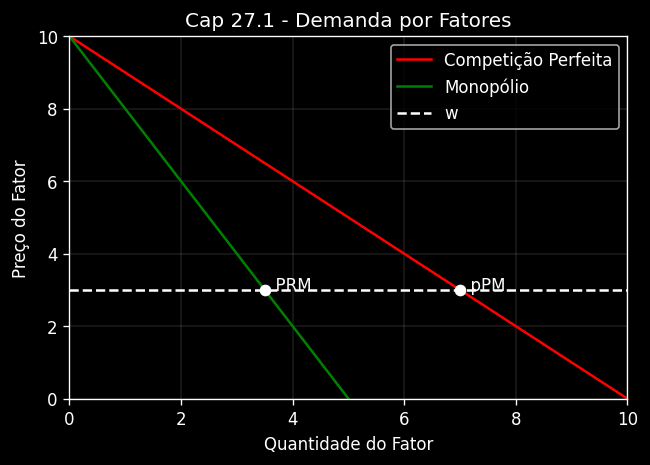
\includegraphics[scale=0.75]{cap27_1-demanda_fatores.png}
\end{figure}

\section{O Monopsônio}

O livro constrói um cenário onde temos um mercado competitivo de fatores, um único comprador e um mercado de produtos competitivo.
\\
\\
Para simplificar, vamos supor que a empresa usa apenas um único fator de produção. Sua função de produção será dada por $y = f(x)$.  A análise de comportamento do monopsônio é parecida com a do monopólio, só que ao invés de impactar o mercado pela oferta de bens, o poder de mercado é exercido pela compra. A quantidade de fator comprado, impactará no preço pago por ele.
\\
\\
Para expandir o modelo, vamos criar uma função de oferta inversa $w(x)$ onde o preço pago pelo insumo será determinado pela quantidade demandada pelo nosso único comprador (chamado de \textbf{monopsonista}). É razoável supor que $\frac{d w(x)}{d x} > 0$.
\\
\\
Como na imagem da seção acima, num mercado de fatores competitivo, a curva de oferta de fatores é plana. Ou seja, não importando a quantidade demanda, o custo será sempre o mesmo. Já no caso de um único comprador, a curva de oferta de fatores será inclinada positivamente. Como o professor resume perfeitamente: "Uma empresa num mercado de fatores competitivo é uma \textbf{tomadora de preços}. Um monopsionista é um \textbf{fixador de preços}".
\\
\\
A maximização de lucro do monoposionista será:

\begin{center}
\LARGE $\stackrel{máx}{\text{\small $x$}} \ \ \stackrel{pf(x) - w(x)x}{\ }$ \\
\end{center}

Ou seja, temos que encontrar a quantidade de insumo - $x$ - que permita maximizar a diferença entre a receita total - $p f(x)$ - e o custo total - $w(x)x$. A condição de primeira ordem desse problema será:

$$ pf'(x) - [ w(x) + w'(x)x ] = 0 $$
$$ pf'(x) = w(x) + w'(x)x $$
$$ \underbrace{pPM_x}_{\textrm{PRM}} = \ \underbrace{w(x) + w'(x)x}_{\textrm{Custo Marginal}} $$
\\
Como supomos no início do nosso caso, o mercado do produto é competitivo. Isso quer dizer que a receita marginal será igual a $pPM_x$ (que é a mesma coisa que $pf'(x)$). Mas obter o custo marginal não será tão simples quanto antes.
\\
\\
Quando a firma compra uma pequena quantidade ($x$) do fator de produção, ela deve pagar o preço desse fator vezes a quantidade ($wx$). Contudo, nesse caso, o preço será afetado exatamente na quantidade demanda ($w'(x)x$). O valor final pago é a soma dessas duas ações. Podemos desenvolver essa lógica exatamente como desenvolvemos a receita do monopolista na seção 25.1.

$$ \Delta c = w \Delta x + x \Delta w $$
$$ \frac{\Delta c}{\Delta x} = w + x \frac{\Delta w}{\Delta x} $$
$$ = w \left[ 1 + \frac{x}{w} \frac{\Delta w}{\Delta x} \right] $$
$$ = w \left[1 + \frac{1}{\eta} \right] $$
\\
Onde $\eta$\footnote{O nome dessa letra grega é eta.} representa a elasticidade da oferta. Como a inclinação a curva de oferta é positiva, $\eta$ será maior que zero. Se a elasticidade da oferta for perfeita, $eta$ será infinito. O que implica, por sua vez, no caso da competição perfeita onde o custo marginal seria igual a $w$. Quaisquer outro valor da elasticidade, produzirá uma curva de oferta não plana.

\subsection{Monopsônio com Oferta Linear}

Para aplicar a teoria precisamos dar alguma forma funcional a nossa curva de oferta do fator de produção. No livro, o professor trabalha com uma oferta linear da seguinte forma:

$$ w(x) = a + bx $$
\\
O custo total da produção será dado por:

$$ C(x) = w(x)x = ax + bx^2 $$
\\
O custo marginal do fator é obtido pela derivada da função custo total em relação ao fator $x$.

$$ CMa_x(x) = a + 2bx $$
\\
Graficamente, a quantidade do insumo demandado será igual ao ponto onde o $PRM = pPM$ é igual ao custo marginal da aquisição do insumo.

\begin{figure}[H]
\centering
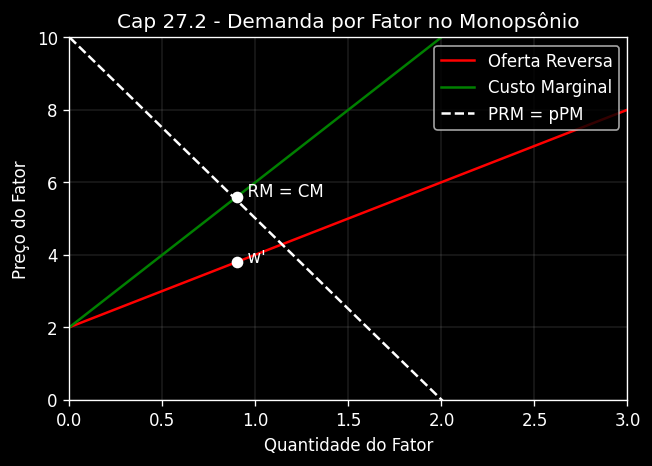
\includegraphics[scale=0.75]{cap27_2-demanda_fatores_monopsonio.png}
\end{figure}

Se o custo marginal for maior que o retorno da receita oriunda do emprego desse fator, o monopsionista não terá o incentivo à utilização do mesmo. Caso o contrário, valerá a pena usar um pouco mais do insumo. O ponto onde não há incentivo a mudança é justamente onde o custo marginal é igual à receita marginal.
\\
\\
Assim como no caso do monopolista, a quantidade demanda será o ponto menor do que se o mercado fosse competitivo. No cenário de competição, a quantidade demandada seria o ponto onde a oferta reversa se equivalesse ao retorno do emprego do insumo (medido pelo $PRM$). Só que nesse caso, a ineficiência acontece no mercado de fatores e não no de produção.
\\
\\
\textbf{Comentário:} Veja o exemplo sobre o salário mínimo que o professor colocou no livro. Você deve ser capaz de entendê-lo sem tanto sofrimento. A conclusão de que no mercado de trabalho controlado por um monopsionista, um salário mínimo pode aumentar o nível de emprego é bem interessante.

\section{Monopólios Upstream e Downstream na Cadeia de Produção}

Nós só observamos dois tipos de concorrência imperfeita. Mas os exemplos acima são apenas um dos múltiplos arranjos que podem acontecer na realidade. O professor não achou serventia em ter que modelar todas as cominações possíveis, e eu não vou fazer isso também. O importante é saber como modelar o comportamento do monopolista (ou do monopsionista) seja no mercado de fatores ou no mercado de produção.
\\
\\
Mesmo não querendo modelar todos os arranjos possíveis, ainda veremos uma nova situação: O caso onde um monopolista no mercado de fatores vende para um monopolista no mercado de produção.
\\
\\
O monopolista do mercado de fatores é chamado de \textbf{upstream} ou \textbf{para trás}. Ele vende o insumo $x$ ao preço $k$ e com custo marginal constante $c$. O monopolista do mercado de produto será denominado por \textbf{downstream} ou \textbf{para frente}. Esse segundo usará o insumo $x$ para obter a produção  $y$ via função de produção da forma $f(x) = y$ que será vendida no mercado cuja demanda inversa será $p(y)$. No nosso exemplo a forma funcional dessa demanda será $p(y) = a - by$.
\\
\\
O professor usa uma simplificação bem camarada da função de produção do downstream. Ele supõe que $f(x) = y = x$, ou seja, é como se ele revendesse o produto\footnote{O que torna esse exemplo surpreendentemente válido para diversas ocasiões da vida real.}. Outra simplificação é que o downstream também terá custo marginal igual ao preço pago pelo insumo ($k$) ao upstream.
\\
\\
Teremos que buscar um equilíbrio entre os dois monopolistas. Para isso, vamos começar modelando o caso para o downstream. Ele quer maximizar seu lucro que é dado pelo seguinte problema:

\begin{center}
\LARGE $\stackrel{máx}{\text{\small $y$}} \ \ \stackrel{L(y)\ =\ p(y)y - ky}{\ }$ \\
\end{center}
\begin{center}
\LARGE $\stackrel{máx}{\text{\small $y$}} \ \ \stackrel{L(y)\ =\ [a - by]y - ky}{\ }$ \\
\end{center}
\begin{center}
\LARGE $\stackrel{máx}{\text{\small $y$}} \ \ \stackrel{L(y)\ =\ ay - by^2 - ky}{\ }$ \\
\end{center}

A condição de primeira ordem da última forma é dada por:

$$ \frac{d L(y)}{d y} = a - 2by - k = 0 $$
$$ a - 2by = k $$
$$ y = \frac{a - k}{2b} $$

Como a função de produção usada iguala a quantidade de insumo à quantidade de produto. Vemos que ele demandará exatamente a mesma quantidade de fator de produção que a oferta no mercado do produto.

$$ x = \frac{a - k}{2b} $$

\textbf{Comentário:} O importante aqui é perceber que a função de produção do monopolista downstream é usada para derivar a demanda do fator produzido pelo upstream. Perceba que a quantidade demandada de fator depende do preço pago por ele e da demanda no mercado de produto. Tudo bem intuitivo e simples.
\\
\\
Agora temos que modelar o comportamento do upstream. Vamos supor que ele tenha acesso à função demanda de fatores do downstream e queira maximizar seu lucro. A demanda inversa de fatores nada mais é do que a última equação tendo k em função de x:

$$ k(x) = a - 2bx $$

A receita é dada por:

$$ k(x)x = ax - 2bx^2 $$

E a receita marginal por:

$$ RM_x = a - 4bx $$

Igualando a receita marginal ao custo marginal, teremos que:

$$ a - 4bx = c $$

ou seja, o total vendido no mercado pelo monopolista upstream será dado por:

$$ x = \frac{a - c}{4b} $$

Como a função de produção é um pra um, podemos definir que o total produzido no mercado de produto será:

$$ y = \frac{a - c}{4b} $$

Essa é a quantidade da produção que maximiza os lucros do monopolista upstream. Mas lembre-se que ele usa como função de demanda de fatores o resultado do problema de maximização do downstream. Então a solução acaba por gerar um lucro fruto do processo de maximização de ambos os monopolistas.
\\
\\
Se houvesse apenas um monopolista em ambos os mercados (imagine que as duas empresas se fundissem) e os custos de produção dos fatores se mantivessem os mesmos. O problema de maximização seria igualar a receita marginal ($a - 2by$) ao custo do fator ($c$). Isso geraria um volume de produção igual à

$$ y_{int} = \frac{a - c}{2b}$$
\\
O monopolista integrado produzirá o dobro que o arranjo com dois monopolistas separados. Mas qual o motivo dessa diferença?
\\
\\
Para entendermos o motivo dessa diferença precisamos lembrar que o monopolista sempre escolherá o ponto que maximiza o seu lucro pela igualdade entre o custo marginal e a receita marginal. A curva de demanda inversa do mercado serve para determinar o preço de equilíbrio que será usado no mercado dada a decisão da quantidade da produção do monopolista.
\\
\\
O caminho usado para encontrarmos o equilíbrio teve uma etapa para cada monopolista:
\begin{itemize}

\item Primeiro usamos a demanda do mercado de produtos para determinar qual a quantidade o monopolista ofertará (e como essa quantidade é função do preço do fator de produção).

\item Depois, usamos a relação entre a quantidade produzida e os insumos para determinar a demanda inversa do mercado de fatores. Essa demanda é usada pelo monopolista upstream para determinar o seu ponto de maximização.

\end{itemize}

Na prática, o monopolista upstream vai cobrar uma quantidade cujo preço de mercado é superior ao custo marginal. Esse preço será o custo que o monopolista downstream usará para maximizar seu lucro. Contudo, quando as empresas se fundem, o novo custo marginal do monopolista do mercado de produto será exatamente o custo de produção $c$. Nós retiramos de cena o Markup do monopolista upstream.

%%%%%%%%%%%%%%%%%%%%%%%% CHAPTER %%%%%%%%%%%%%%%%%%%%%%%%
\chapter{O Oligopólio}

\begin{chapquote}{The Godfather}
	``I want you to talk to this movie bigshot and settle this business for Johnny. Now, if there's nothing else, I'd like to go to my daughter's wedding.''
\end{chapquote}


O trabalho de entender os mercados é longo e trabalhoso. Até agora, nós elaboramos as estruturas mais simples e que se encontram nos dois extremos do poder de mercado. De um lado, aprendemos a estrutura onde não existe poder de mercado e as empresas são pequenas concorrentes. Após isso, vimos o que acontece quando temos apenas uma empresa (ou empresas que trabalham como se fossem uma só) e o poder de mercado está todo nas mãos dela.
\\
\\
Agora vamos entrar num cenário um pouco mais realista. Pensemos em uma situação onde temos poucos concorrentes. De um lado, não temos tantos a ponto de ninguém poder manipular seus preços. Do outro, ninguém é grande o suficiente para ignorar o comportamento dos seus concorrentes. Esse arranjo é denominado de \textbf{Oligipólio}.
\\
\\
Nós já tangenciamos esse assunto quando vimos o modelo de concorrência monopolística no capítulo 25. Esse arranjo também é um tipo de oligopólio. Nessa configuração, as variáveis mais importantes são o custo de entrada (pela regra do custo médio) e nas estratégias de diferenciações entre os produtos (seja a de convergência ou a de diferenciação).
\\
\\
Aqui vamos estudar arranjos com um número ainda menor de concorrentes. Como dito anteriormente, a medida que aprimoramos o nosso modelo, as características únicas de cada mercado se tornam cada vez mais relevantes. Aqui só vamos conseguir ver regras gerais de resultados possíveis, bem como, algumas variáveis importantes para monitorarmos.
\\
\\
Vamos partir da estrutura de competição de apenas duas empresas: o \textbf{Duopólio}\footnote{Alguns exemplos em que podemos aproximar esse modelo: PS4 x Xbox, Iphone x Samsung, Coca-Cola x Pepsi, Apple x Microsoft.}. Outra limitação que imporemos é a de que os produtos são idênticos. Essas limitações nos livram de notações complexas com várias competidores e a utilização do poder de mercado oriundo da diferenciação. Nosso foco são as \textbf{interações estratégicas}.\footnote{Se você quiser ver modelos mais próximos da realidade, vai ter que encarar um mestrado e um doutorado.}

\section{A Escolha de Uma Estratégia}

Em um arranjo de dois competidores, temos que desenvolver um modelo que consiga equilibrar 4 variáveis:

\begin{itemize}
\item Preço da Empresa 1
\item Preço da Empresa 2
\item Quantidade da Empresa 1
\item Quantidade da Empresa 2
\end{itemize}

Na hora de tomar uma decisão sobre o preço e a quantidade, uma empresa pode, ou não, ter acesso as escolhas feitas pelo seu concorrente. Chamaremos de \textbf{líder} toda empresa que decidir seu \textbf{preço} ou \textbf{quantidade} antes da outra. A empresa que decidirá após a informação da decisão da empresa líder será chamada de \textbf{seguidora}. As interações desse tipo são chamadas de \textbf{jogos sequenciais}.\footnote{Começamos a chegar mais perto da teoria dos jogos.}
\\
\\
Quando as duas empresas decidem sem ter acesso a informação do adversário, elas precisam supor o que ele fará. Esse arranjo é denominado \textbf{jogo simultâneo}.
\\
\\
Com esses dois conceitos, podemos ter 4 tipos de interações estratégicas:

\begin{itemize}
\item Liderança de Preço
\item Liderança de Quantidade
\item Preço Simultâneo
\item Quantidade Simultânea
\end{itemize}

Analisaremos cada tipo de interação estratégica que surge com cada tipo de esquema. Mas não pararemos ai. Uma opção possível de estratégia é a de negociação entre as empresas para formação de um \textbf{conluio}. Esse tipo de esquema é chamado de \textbf{jogo cooperativo}.
\\
\\
\textbf{Comentário:} Leia o exemplo da estratégia de "cobrimos o preço da concorrência"\ e a partir de agora, você nunca mais lerá essas ofertas com os mesmos olhos.

\section{Liderança de Quantidade}

O modelo desenvolvido nessa seção é creditado ao economista alemão Heinrich von Stackelberg. Seu livro \textit{Marktform und Gleichgewicht} foi publicado em 1934.\footnote{Eu recomendo dar uma olhada na bibliografia dos gigantes que desenvolveram as teorias ao longo desse livro.}.
\\
\\
Vamos supor que temos uma empresa líder na quantidade. Como é de se esperar, ela fixará sua produção em $y_1$ unidades. A empresa seguidora, de posse da informação de $y_1$ e da demanda inversa do mercado, escolherá seu nível de produção em $y_2$. A demanda inversa do mercado será em função do total de produtos $p(Y) = p(y_1 + y_2)$.
\\
\\
Como a empresa líder decidirá sua quantidade de modo a maximizar seus lucros? Certamente ela terá que supor como a empresa seguidora agirá. Não seria nada estranho que ela tivesse a hipótese que a empresa seguidora queira maximizar seus lucros também . Desse modo, a empresa líder terá que endogenizar o problema da maximização do lucro da empresa seguidora.

\subsection{O Problema da Empresa Seguidora}

O problema da maximização da empresa seguidora é:

\begin{center}
\LARGE $\stackrel{máx}{\text{\small $y_2$}} \ \ \stackrel{p(y_1 + y_2)y_2 - c_2(y_2)}{\ }$ \\
\end{center}

Já conhecemos esse tipo de problema muito bem. Queremos encontrar o ponto onde a receita marginal será igual ao custo marginal.

$$ RM_2 = CMa_2 = p(y_1 + y_2) + \frac{dp(y_1+y_2)}{dy_2}y_2 - \frac{dc_2(y_2)}{y_2} = 0  $$

ou, na notação de derivadas de Lagrange

$$ RM_2 = CMa_2 = p(y_1 + y_2) + p'(y_1 + y_2)y_2 - c'(y_2) = 0  $$

A novidade aqui é que temos que levar em consideração a quantidade $y_1$ para encontrar nosso $y_2$. Isso quer dizer que 

$$y_2 = f_2(y_1)$$

Nós conseguimos obter essa função isolando nosso termo $y_2$ no problema de maximização acima. Essa função tem o nome de \textbf{função de reação} e nos diz qual quantidade será produzida pela empresa seguidora ao ser conhecida a quantidade da empresa líder.
\\
\\
Para prosseguirmos vamos ter que definir uma forma funcional à nossa função de demanda inversa. Faremos para o caso linear onde $p(y_1 + y_2) = a - b(y_1 + y_2)$. Também adotaremos o custo igual a zero para facilitar a matemática da coisa.

$$\textrm{Função Lucro 2: } \pi_2(y_1,y_2) = p(y_1 + y_2)y_2$$
$$ = [a - b(y_1 + y_2)]y_2 = ay_2 - by_1 y_2 - by_2^2 $$

Com a função de lucro e a de reação, conseguimos ver a relação entre essas duas funções. Na imagem abaixo podemos ver que a curva de reação sempre atravessa as curvas de isolucro no ponto onde temos o maior valor de $y_2$.

\begin{figure}[H]
\centering
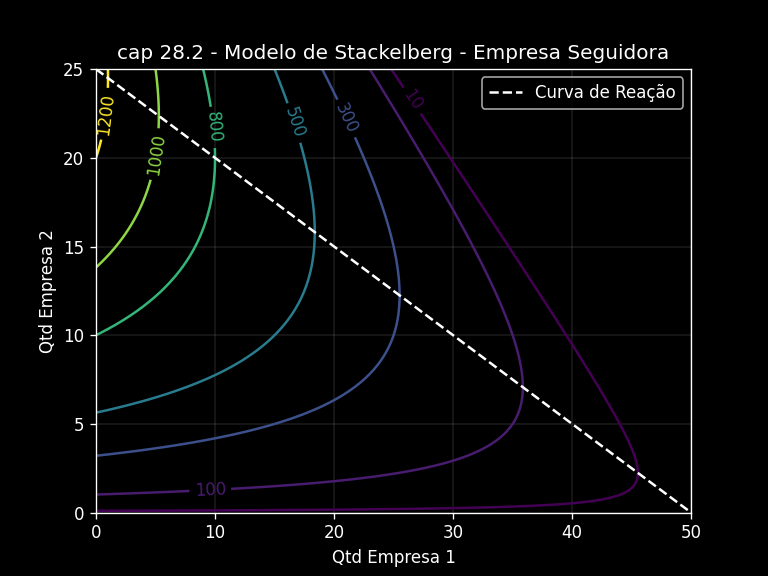
\includegraphics[scale=0.75]{cap28_2-modelo_stackelberg_parcial.png}
\end{figure}

\subsection{O Problema da Empresa Líder}

Já aprendemos a parte do modelo que trata da quantidade de equilíbrio dada a escolha anterior da empresa líder. Agora vamos desenvolver como essa empresa define a sua quantidade de modo a maximizar o seu lucro.
\\
\\
Uma das características desse modelo é que a empresa líder sabe como a outra empresa vai se comportar dada a escolha dela, ou seja, ela conhece $f_2(y_1)$. Diante disso, o problema da maximização dela está sujeita a essa restrição.

\begin{center}
\LARGE $\stackrel{máx}{\text{\small $y_1$}} \ \ \stackrel{p(y_1 + y_2)y_1 - c_1(y_1)}{\ }$ \\
\small de modo que \normalsize $y_2 = f_2(y_1)$
\end{center}

Ou melhor, podemos colocar tudo em função de $y_1$ e obtermos

\begin{center}
\LARGE $\stackrel{máx}{\text{\small $y_1$}} \ \ \stackrel{p[y_1 + f_2(y_1)]y_1 - c_1(y_1)}{\ }$ \\
\end{center}

A produção total será definida pela líder sendo que será parte devida a produção direta e a outra parte pela resposta da seguidora ao nível definido da produção, ou seja, $y_1 + f_2(y_1)$. Pela equação da demanda inversa linear, temos que a função de reação da empresa seguidora é

$$ f_2(y_1) = y_2 = \frac{a - by_1}{2b}$$

A função lucro é dada pela receita menos os custos (que no nosso exemplo é zero)

$$ \textrm{Função Lucro 1: } \pi(y_1,y_2) = [a - b(y_1 + y_2)]y_1 = ay_1 -by_1^2 - by_1y_2 $$

Colocando a função de reação dentro da função de lucro teremos

$$ = ay_1 -by_1^2 - by_1f(y_1)$$
$$ = ay_1 -by_1^2 - by_1\frac{a - by_1}{2b}$$
$$ = ay_1 -by_1^2 - \frac{\cancel{b}y_1a}{2\cancel{b}} + \frac{\cancel{b}*b(y_1)^2}{2\cancel{b}}$$
$$= ay_1 -by_1^2 - \frac{ay_1}{2} + \frac{by_1^2}{2}$$
$$ \pi(y_1,y_2) = \frac{a}{2}y_1 - \frac{b}{2}y_1^2$$

Para encontrarmos a quantidade ótima basta derivar a função lucro em função de $y_1$ e igualar a zero. O que nos dará 

$$ y_1^* = \frac{a}{2b} $$

Desse modo, podemos encontrar facilmente a produção de equilíbrio da empresa seguidora.

$$ y_2^* = \frac{a - by_1}{2b} $$
$$ y_2^* = \frac{a - b(a/2b)}{2b} $$
$$ y_2^* = \frac{a - ab/2b}{2b} $$
$$ y_2^* = \frac{2ab/2b - ab/2b}{2b} $$
$$ y_2^* = \left( \frac{2ab}{2b} - \frac{ab}{2b} \right) \frac{1}{2b} $$
$$ y_2^* = \left( \frac{\cancel{2}a\cancel{b}}{\cancel{2b}} - \frac{a\cancel{b}}{2\cancel{b}} \right) \frac{1}{2b} $$
$$ y_2^* = \left( a - \frac{a}{2} \right) \frac{1}{2b}$$
$$ y_2^* = \frac{a}{4b} $$

Por fim, podemos ter a quantidade total do mercado pela soma de $y_1^* + y_2^* = \frac{3a}{4b}$. Agora que temos a função de lucro da empresa 1, podemos acrescentar as curvas de isolucro para vermos a solução gráfica da álgebra que acabamos de desenvolver.

\begin{figure}[H]
\centering
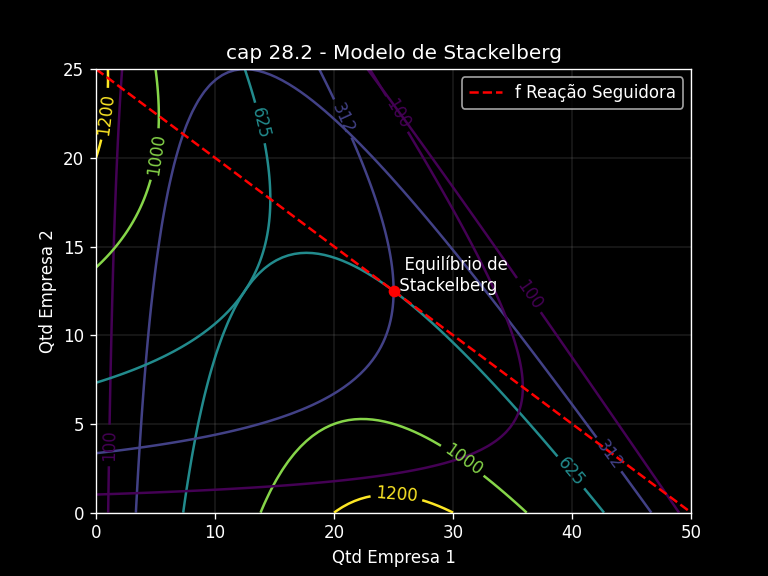
\includegraphics[scale=0.75]{cap28_2-modelo_stackelberg_completo.png}
\end{figure}

Se você colocar as quantidades de equilíbrio nas equações de lucro, chegará nos valores de lucro para cada empresa desse modelo. O ponto de Equilíbrio de Stackelberg acontecerá onde a curva de reação tangencia a maior curva de isolucro da empresa líder. No exemplo da imagem eu usei para a função da demanda inversa linear um $a = 100$ e um $b = 2$.

\section{Liderança do Preço}

Outra forma de um jogo sequencial acontecer entre duas empresas é pela definição do preço pela empresa líder. Similarmente ao que vimos na seção anterior, a empresa líder precisa levar em consideração o que a empresa seguidora fará.

\subsection{O Problema da Seguidora}
No mercado competitivo, o preço é dado e as empresas maximizam seus lucros pela igualdade entre a a receita marginal (que é justamente o preço) e o custo marginal. Por sorte, o problema da empresa seguidora é bem parecido com esse. Ela recebe o preço definido pela líder e maximiza seu lucro.

\begin{center}
\LARGE $\stackrel{máx}{\text{\small $y_2$}} \ \ \stackrel{py_2 - c_2(y_2)}{\ }$ \\
\end{center}

A oferta da empresa seguidora será a quantidade que iguala o preço definido pela líder ao custo marginal.

\subsection{O Problema da Líder}

A empresa líder, sabendo a função de oferta da empresa seguidora, vai trabalhar com a diferença entre a Demanda do mercado e a demanda da empresa seguidora, ou seja, $R(p) = D(p) - S(p)$. O nome dessa curva de demanda reduzida é \textbf{curva de demanda residual}.
\\
\\
Supondo um custo de produção constante $c$. A função de lucro da empresa líder é dada por

$$ \textrm{Função Lucro 1: } \pi_1(p) = R(p)p - R(p)c = (p - c)R(p)  $$

A maximização dessa empresa acontece onde a receita marginal (que nesse caso é oriunda da demanda residual) é igual ao custo marginal. 
\\
\\
A partir de agora temos que definir uma forma funcional para a nossa curva de demanda, como sempre, vamos optar pelo caso mais simples, $D(p) = a - bp$. Também vamos definir as funções custo para a seguidora $c_2(y_2) = y_2^2/2$ e para a líder $c_1(y_1) = cy_1$.
\\
\\
Isso nos diz que a condição de maximização da empresa seguidora será a derivada da função lucro igual a zero.

$$ \frac{d L(y_2)}{y_2} = p - \frac{2y_2}{2} = 0 $$
$$ = p - y_2 = 0 $$
$$ = p = y_2 $$

Ou seja, nossa função de oferta da seguidora será $S(p) = p$. De posse dessa informação, podemos descobrir a equação da demanda residual da empresa líder pela subtração da curva de demanda pela oferta da seguidora.

$$ R(p) = D(p) - S(p) = a - bp - p = a - (b + 1)p $$

Agora é só maximizar o lucro pela igualdade entre a receita marginal e o custo marginal e verificar na curva de demanda inversa o volume de produção e o preço. A demanda inversa é obtida isolando $p$ da demanda residual.

$$ p(y_1) = \frac{a}{b+1}-\frac{1}{b+1}y_1 $$

A receita da empresa líder é obtida pela multiplicação de $p(y_1)$ por $y_1$. A receita marginal é a derivada dessa função em relação a $y_1$.

$$ Receita_1: \left[ \frac{a}{b+1} - \frac{1}{b+1}y_1 \right] y_1 $$
$$ = \frac{a}{b+1}y_1 - \frac{1}{b+1}y_1^2 $$

A receita marginal será

$$ RMa_2 = \frac{a}{b+1} - \frac{2}{b+1}y_1 $$

O nosso custo foi definido como $c_1(y_1) = cy_1$, logo, o custo marginal é igual a $c$\footnote{A essa altura do campeonato você não tem mais dúvida nessas derivadas triviais né?!}.
\\
\\
Portanto, nosso problema de maximização será dado pela equação

$$ \frac{a}{b+1} - \frac{2}{b+1}y_1 = c $$
$$ - \frac{2}{b+1}y_1 = c - \frac{a}{b+1} $$
$$ \frac{2}{b+1}y_1 = \frac{a}{b+1} - c $$
$$ \frac{2}{b+1}y_1 = \frac{a}{b+1} - \frac{c(b+1)}{b+1} $$
$$ \frac{2}{\cancel{b+1}}y_1 = \frac{c(b+1)}{\cancel{b+1}} $$
$$ 2y_1 = c(b+1) $$
$$ y_1^* = \frac{c(b+1)}{2} $$

Na imagem abaixo, nós podemos ver as variáveis interagindo. A oferta total será a soma das quantidades de ambas empresas.

\begin{figure}[H]
\centering
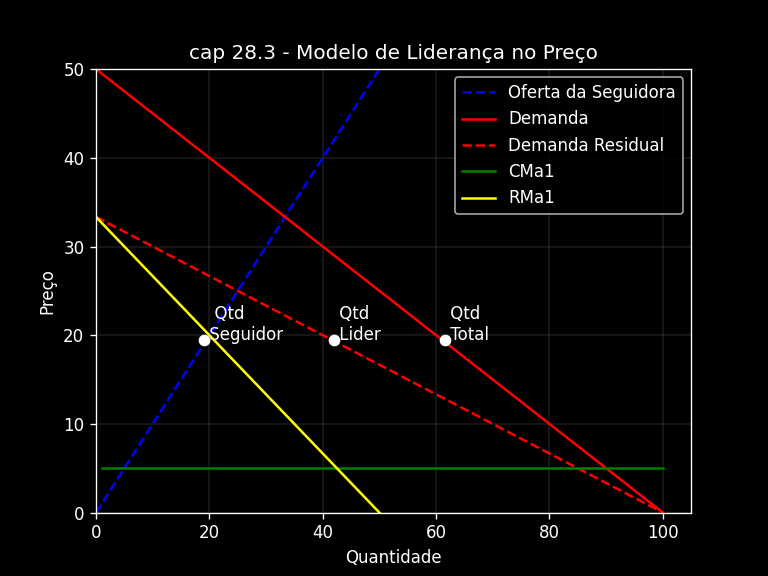
\includegraphics[scale=0.75]{cap28_3-lideranca_preco.png}
\end{figure}

\section{Comparação entre as Lideranças de Preço e Quantidade}

Esse seção do livro é bem explicativa. Vá ler o material original.

\section{Estabelecimento Simultâneo da Quantidade}

Não raramente, as empresas não ficam se comunicando entre si para informar seus concorrentes a respeito de suas decisões . Nesses cenários, as empresas precisam supor o que suas concorrentes farão. Esse modelo é chamado de \textbf{Modelo de Cournot} e é um modelo de jogo simultâneo onde as empresas definem suas quantidades produzidas e vendidas no mercado.
\\
\\
Como de costume, suporemos que as empresas queiram maximizar seus lucros. Pensemos no caso da empresa 1. A quantidade total do mercado será dada por $Y = y_1 + y_2^e$, onde $y_2^e$ é a quantidade prevista da empresa 2. O preço de equilíbrio do mercado será dado pela equação de demanda inversa $p(Y) = p(y_1 + y_2^e)$.
\\
\\
O problema de maximização do lucro será

\begin{center}
\LARGE $\stackrel{máx}{\text{\small $y_1$}} \ \ \stackrel{p(y_1 + y_2^e)y_1 - c(y_1)}{\ }$ \\
\end{center}

Não é difícil ver que quaisquer expectativa da produção da sua concorrente mudará o ponto de produção que maximizaria o lucro. Desse modo, podemos ver que existe uma relação entre essa expectativa e a produção, de modo mais formal, $y_1 = f(y_2^e)$.
\\
\\
Mas, espera um pouco, a gente já viu algo bem parecido um pouco mais acima. Essa é a \textbf{curva de reação} da empresa, a diferença é que aqui a empresa 1 não é mais a líder e essa reação se refere a \textit{expectativa} da produção. Mas o tratamento matemático é o mesmo.\footnote{Para a nossa sorte!}
\\
\\
Similarmente, a empresa 2 se depara com a mesma situação.

$$y_2 = f(y_1^e)$$

Como ambas maximizações são funções de expectativas, é muito mais provável que as empresas não acertem exatamente o volume de produção da sua concorrente. O equilíbrio de Cournot é dado pelo sistemas de equações

$$ y_1^* = f_1(y_2^*) $$
$$ y_2^* = f_2(y_1^*) $$

Nessa solução, nenhuma das empresas terá incentivos em mudar seu nível de produção.

\section{Exemplo do Equilíbrio de Cournot}

Se reutilizarmos o exemplo na liderança da quantidade (com custo zero e demanda linear) obteremos as mesmas funções de reação que a empresa 2 tinha naquele modelo.

$$ y_1 = \frac{a - by_2^e}{2b} $$

e

$$ y_2 = \frac{a - by_1^e}{2b} $$

O ponto de equilíbrio acontece onde $y_1 = y_2$, ou seja, onde as curvas de reação são iguais. Nesse ponto, $y_1^e = y_1$ e $y_2^e = y_2$. Só precisamos substituir dentro desse sistema de equações do seguinte modo

$$ y_1 = \frac{a - by_2^e}{2b} $$
$$ y_1 = \frac{a - by_2}{2b} $$
$$ y_1 = \frac{a - b(\frac{a - by_1}{2b})}{2b} $$
$$ y_1 = \frac{a - (\frac{ab - b^2y_1)}{2b})}{2b} $$
$$ y_1 = \frac{\frac{2ba}{2b} - (\frac{ab - b^2y_1)}{2b})}{2b} $$
$$ y_1 = \frac{2ba - ab + b^2y_1}{2b}\frac{1}{2b} $$
$$ y_1 = \frac{2ba - ab + b^2y_1}{4b}\frac{1}{b} $$
$$ y_1 = \frac{2\cancel{b}a - a\cancel{b} + b^{\cancel{2}}y_1}{4\cancel{b}}\frac{1}{b} $$
$$ y_1 = \frac{2a - a + by_1}{4b} $$
$$ 4by_1 - by_1 = a $$
$$ 3by_1 = a $$
$$ y_1^* = \frac{a}{3b} = y_2^* $$

Com essas funções e as equações de lucro podemos ver graficamente o equilíbrio de Cournot onde as curvas de reação se equivalem.

\begin{figure}[H]
\centering
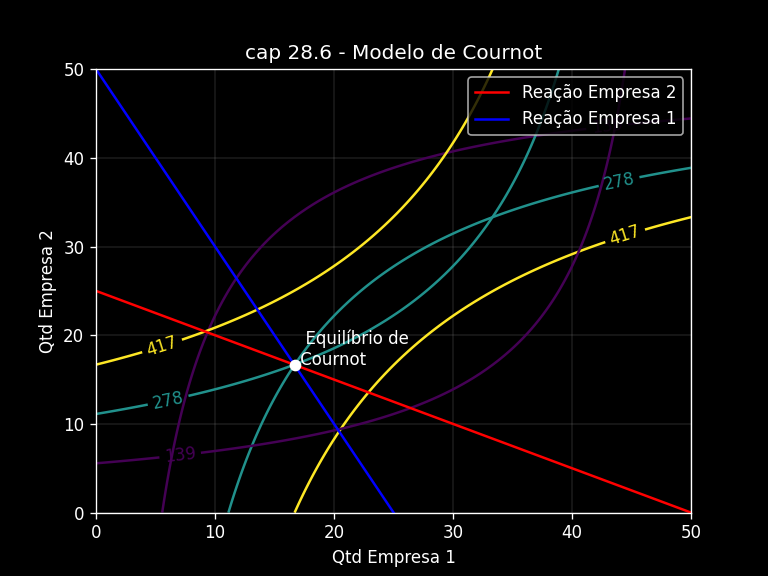
\includegraphics[scale=0.75]{cap28_6-modelo_cournot.png}
\end{figure}

\section{Ajustamento para o Equilíbrio}

Seria muita boa vontade supor que, na vida real, as empresas conseguissem acertar na mosca o nível de produção dos seus concorrentes. Mas o nosso modelo é forte o suficiente para um processo de ajustamento em caso de (prováveis) palpites equivocados no nível de produção.
\\
\\
Imaginemos que as empresas suponham que a produção do seu concorrente será uma quantidade qualquer diferente do equilíbrio. Para facilitar, vamos supor que a cesta inicial produzida esteja em cima da curva de reação da empresa 2. A cesta inicial, que chamamos no gráfico de $Cesta(t)$ será igual à lista $(y_1^t,y_2^t)$.
\\
\\
Essa cesta está na curva de reação da empresa 2, logo, essa empresa não terá incentivo a fazer nenhuma mudança. Mas para a empresa 1, a situação é outra, ela quer reduzir sua produção para aumentar seus lucros.
\\
\\
Isso faz com que a cesta do mercado se desloque para a curva de reação da empresa 1. Mas agora, quem está insatisfeito é a empresa 2. Ela fara um reajuste, só que agora, usará a nova produção da empresa 1 para definir sua oferta.
\\
\\
Esse processo fica se realimentando até um ponto onde elas estão satisfeitas. Nós já vimos agora a pouco que esse ponto é justamente o equilíbrio do modelo de Cournout.
\\
\\
A imagem abaixo mostra esse caminho. Mas eu também transformei ela em um gif animado\footnote{Com alguma dose de bom humor.} para ilustrar o caminho até o equilíbrio.

\begin{figure}[H]
\centering
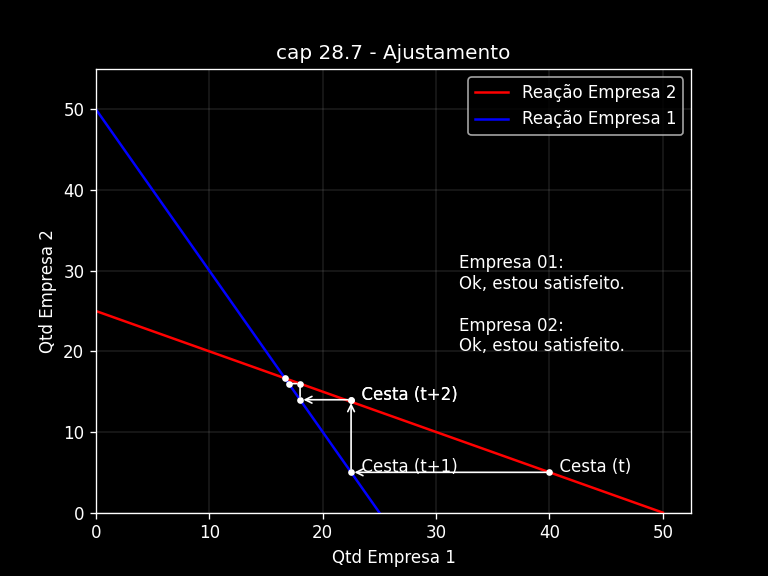
\includegraphics[scale=0.75]{cap28_7-ajustamento.png}
\end{figure}

Essa propriedade de convergência ao ponto de equilíbrio é o que caracteriza esse modelo como um modelo de \textbf{equilíbrio estátvel}. Embora o processo descrito aqui seja bem resumido e simplificado devido o escopo do nosso curso.

\section{Várias Empresas no Equilíbrio de Cournot}

Além de fornecer um modelo para um duopólio, podemos ajustar o modelo de Cournot para $n$ empresas competidoras. A oferta total da indústria será dada por $Y = y_1 + y_2 + \dots + y_{n-1} + y_n$. Desse modo o problema da maximização da empresa será dado pela igualdade entre a receita marginal e o seu custo marginal do seguinte modo

$$ p(Y) + \frac{\delta p}{\delta Y} y_i = CMa(y_i) $$
$$ p(Y) + \frac{\delta p}{\delta Y} \frac{Y}{Y} \frac{p(Y)}{p(Y)} y_i = CMa(y_i) $$
$$ p(Y) \left[1 + \frac{\delta p}{\delta Y} \frac{Y}{p(Y)} \frac{y_i}{Y} \right] = CMa(y_i) $$

Definindo $s_i = \frac{y_i}{Y}$ como a participação da empresa no total do mercado.

$$ p(Y) \left[1 + \frac{\delta p}{\delta Y} \frac{Y}{p(Y)} s_i \right] = CMa(y_i) $$

O termo $p(Y)$ é a curva de demanda. Então, se lembrarmos da fórmula da elasticidade, podemos ver que o termo $\frac{\delta p}{\delta Y} \frac{Y}{p(y)}$ é justamente o inverso da elasticidade $\frac{1}{\epsilon(Y)}$

$$ p(Y) \left[1 + \frac{s_i}{\epsilon(Y)} \right] = CMa(y_i) $$

Como a elasticidade de demanda é negativa

$$ p(Y) \left[1 - \frac{s_i}{|\epsilon(Y)|} \right] = CMa(y_i) $$

O professor faz uma transformação que, para alguns, pode parecer estranha. Mas a lógica é essa (se tiver difícil de ver, dá um zoom):

$$ \frac{1}{\frac{\epsilon(Y)}{s_i}} = \frac{\frac{1}{1}}{\frac{\epsilon(Y)}{s_i}} = \frac{1}{1} \frac{s_i}{\epsilon(Y)} = \frac{s_i}{\epsilon(Y)} $$

Com essa transformação, chegamos em

$$ p(Y) \left[1 - 1/\frac{|\epsilon(Y)|}{s_i} \right] = CMa(y_i) $$

Essa solução é bem parecida com a maximização do monopolista. A principal diferença é esse termo $s_i$ dividindo a elasticidade. Como $s_i = y_i/Y$ ele será $0 \leq s_i \leq 1$. No caso monopolista, sabemos que $s_i = 1$. No outro extremo, se $lim (s_i) \rightarrow 0$, a empresa terá elasticidade infinita como as empresas da competição perfeita.  
\\
\\
Para as empresas não monopolísticas e com algum poder de mercado, podemos entender esse termo como a elasticidade da demanda da empresa. Quanto maior $s_i$ menor será a elasticidade da demanda da empresa.
\\
\\
Isso nos mostra que, em um mercado competitivo, temos um equilíbrio de Cournot. As empresas estarão maximizando seus lucros sem incentivo em mudar seu nível de produção.

\section{Fixação Simultânea de Preços}

Da mesma maneira que conseguimos desenvolver um modelo para quantidade e preço em jogos sequenciais, podemos fazê-lo para os jogos simultâneos. Já aprendemos nessa última seção como as empresas definem as quantidades produzidas de modo a maximizar seus lucros sem que haja uma empresa líder no processo.
\\
\\
Acontece que, em algum momento do século XIX, um matemático francês de nome Joseph Bertrand, ao ler o livro do Cournot, desenvolveu um modelo simultâneo de equilíbrio de preços. Esse modelo ficou conhecido como \textbf{concorrência de Bertrand}.
\\
\\
Assim como fizemos com Cournot, estamos na busca do par de preços que permitam ambas as empresas maximizar seus lucros. Para isso, temos que seguir algumas regras que já fazem parte dos modelos usados até o momento ao longo de todo o livro:

\begin{itemize}
\item O preço não poderá ser maior que o custo marginal. Porque as empresas aumentariam seus lucros simplesmente produzindo menos.
\item Se o preço for maior que o custo marginal, todas as empresas terão um incentivo de reduzir seu preço para "roubar"\ os clientes das concorrentes e ainda auferir lucros positivos.
\end{itemize}

O segundo ponto funciona de maneira recursiva. Se uma empresa reduz seu preço em $10\%$ abaixo dos preços das suas concorrentes, ela ganhará parte do mercado. As concorrentes terão o incentivo em reduzir mais ainda seus preços até o ponto onde não poderão mais reduzir (determinado pelo custo marginal).

\section{Conluio}	

Até agora, todas as soluções envolveram processos de competição entre as empresas. Contudo, não seria nem um pouco alheio à realidade supor que algumas empresas queiram operar de modo coordenado. Esse arranjo é chamado de \textbf{Cartel} e é crime em vários países.
\\
\\
Você já sabe, desde o capítulo 25, que um cartel não passa de um grupo de empresas se comportando como um monopolista. Diante disso, seu problema de maximização será muito parecido com o modelo do capítulo que tratamos sobre o monopólio.
\\
\\
O problema da maximização para um cartel de duas empresas será dado por

\begin{center}
\LARGE $\stackrel{máx}{\text{\small $y_1,y_2$}} \ \ \stackrel{p(y_1+y_2)[y_1 + y_2] - c_1(y_1) - c_2(y_2)}{\ }$ \\
\end{center}

Cujas condições de primeira ordem serão

$$p(y_1^* + y_2^*) + \frac{\delta p}{\delta Y}[y_1^* + y_2^*] = CMa_1(y_1^*)$$
$$p(y_1^* + y_2^*) + \frac{\delta p}{\delta Y}[y_1^* + y_2^*] = CMa_2(y_2^*)$$

Podemos ver que, quando uma empresa decide expandir sua produção, receberá uma quantia oriunda da venda dos seus produtos, contudo, essa oferta adicional reduzirá o preço de equilíbrio do mercado (o que reduz o lucro recebido). A novidade aqui é que essa redução do preço impactará também na outra empresa do cartel.
\\
\\
O que as duas equações anteriores nos dizem é que as quantidades produzidas (e ofertadas no mercado) serão as que igualem seus custos marginais $CMa_1(y_1^*) = CMa_2(y_2^*)$. 
\\
\\
Agora temos um fator interessante para pensarmos. Se uma empresa possuir uma estrutura de custos que permita produzir mais com o mesmo custo marginal que sua empresa companheira, ela obterá uma maior parte dos lucros do mercado. Uma vez que sua produção será maior.

\subsection{O problema da `Desonestidade'}

Será que as empresas que operam em um cartel possuem algum incentivo em "trapacear"\ a sua empresa parceita?\footnote{Nessas situações cabe o didato popular: "Ladrão que rouba ladrão tem ..."}
\\
\\
Vejamos o que acontece com a empresa 1 do nosso cartel, caso ela aumente a sua produção em $\delta y_1$ unidades. Podemos mensurar esse impacto pela derivada parcial da função lucro do cartal em relação a $y_1$

$$ \frac{\partial \pi_1}{\partial y_1} = p(y_1^* + y_2^*) + \frac{\delta p}{\delta Y}y_1^* - CMa_1(y_1^*) $$ 

A condição de maximização do cartel nos diz que

$$ p(y_1^* + y_2^*) + \frac{\delta p}{\delta Y}y_1^* + \frac{\delta p}{\delta Y}y_2^* - CMa_1(y_1^*) = 0 $$ 

Apenas isolando o termo referente à produção da empresa, temos então

$$ p(y_1^* + y_2^*) + \frac{\delta p}{\delta Y}y_1^* - CMa_1(y_1^*) = - \frac{\delta p}{\delta Y}y_2^* $$ 

Como $\delta p / \delta Y$ é negativo, então o termo da esquerda da última equação é positivo. Ou seja, a empresa 1 consegue aumentar seus lucros positivamente ao aumentar sua produção para além do ponto de equilíbrio do cartel.
\\
\\
Aqui mora o problema de longo prazo dos carteis. Na solução de maximização do lucro conjunto, existe um incentivo para cada empresa aumentar sua produção, visto que, se a outra empresa mantiver fixa a sua produção, sempre será lucrativo um aumento unilateral da quantidade produzida.
\\
\\
Agora, se houver desconfiança entre as empresas, fica mais difícil ainda manter a coalizão. Se as empresas esperam que a outra irá aumentar sua produção, elas terão um incentivo adicional em agir antes da outra e aproveitar os lucros positivos oriundos do aumento da produção.
\\
\\
Para exemplificar, vamos pegar uma demanda linear do tipo $p(Y) = a - b(y_1 + y_2)$ e supormos um custo marginal igual a $0$. A equação do lucro será dada por 

$$\pi(y_1,y_2) = p(Y)(y_1 + y_2) = [a - b(y_1 + y_2)](y_1 + y_2) = a(y_1 + y_2) - b(y_1 + y_2)^2$$

A condição de primeira ordem desse problema é dada pela derivada dessa função em relação a $(y_1 + y_2)$. O que nos dá

$$a - 2b(y_1 + y_2) = 0$$
$$y_1^* + y_2^* = \frac{a}{2b}$$

O gráfico abaixo ilustra exatamente esse situação para $a = 100, b = 2$ e os custos de produção fixos em $10$. Veja como temos 3 pontos onde as curvas de isolucro se tocam. Esses pontos ocorrem na reta de maximização do lucro dada pela equação acima.

\begin{figure}[H]
\centering
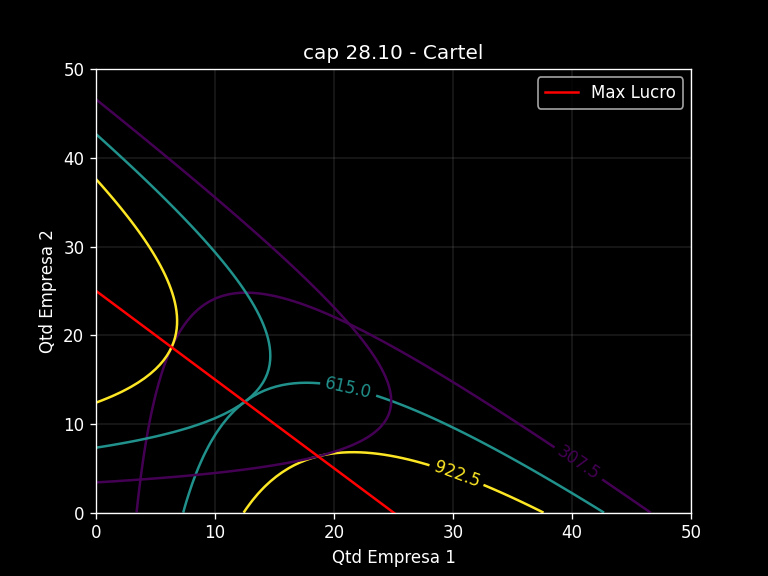
\includegraphics[scale=0.75]{cap28_10-cartel.png}
\end{figure}

Todas as soluções de maximização do lucro acontecem nas tangências das curvas de isolucro que ocorrem na reta de maximização.

\section{Estratégias Punitivas}

Já aprendemos o motivo dos carteis terem alguma dificuldade de se manter estáveis devido os incentivos que as empresas têm de aumentar suas produções. Para superar essa dificuldade, os carteis precisam de medidas para punir quaisquer comportamentos que venham "burlar" o ponto de maximização do lucro da coalizão.
\\
\\
Uma maneira possível é pensar que, em um duopólio, uma das empresas ameace a outra que produzirá permanentemente o nível de produção de Cournot (ou seja, um ponto na curva de reação). Essa estratégia é chamada de \textbf{estratégia de punição}.
\\
\\
Para sabermos se essa punição seria forte o suficiente para mitigar o risco de trapaça, precisamos comparar o que aconteceria com o lucro das empresas nos dois casos. Na coalizão, o lucro $\pi_m$ é dado pela equação de maximização da seção passada. Já no equilíbrio de Cournot, as empresas produzirão o ponto de equilíbrio que produzirá o lucro $\pi_c$.
\\
\\
Os lucros obtidos pelo cartel são maiores porque fazem uso do poder de mercado do monopólio (via markup do custo marginal). Enquanto na solução de Cournot, as quantidades são definidas pela maximização das empresas via ajuste competitivo. Isso implica em lucros menores no segundo modelo se comparados aos lucros do primeiro, ou seja, $\pi_m > \pi_c$.
\\
\\
Se uma empresa do duopólio decidir furar a regra da cota de produção, terá lucros positivos de $\pi_d > \pi_m$. As empresas do monopólio possuem um incentivo de realizar esses lucros via aumento unilateral da produção.
\\
\\
Ao produzir a quantidade do cartel, cada empresa aufere um fluxo constante de lucro $\pi_m$. O valor presente desse fluxo de lucros a partir de hoje é dado por
$$ \textrm{Valor Presente Cartel = } \pi_m + \displaystyle \sum^{\infty}_{i = 1} \frac{\pi_m}{(1 + r)^i} = \pi_m + \pi_m \displaystyle \sum^{\infty}_{i = 1} \frac{1}{(1 + r)^i} $$

Definindo $\displaystyle \sum^{\infty}_{i = 1} \frac{1}{(1 + r)^i}$ como $1/r$. Podemos resumir a equação acima como está no livro

$$ \textrm{Valor Presente Cartel = } \pi_m + \frac{\pi_m}{r} $$

Enquanto o valor presente da empresa que decida fraudar o cartel e recebe o equilíbrio de Cournot como resultado

$$ \textrm{Valor Presente Trapaça = } \pi_d + \frac{\pi_c}{r} $$

Quando valerá a pena trapacear e quando será melhor se manter fiel ao cartel? Não é difícil ver que se o valor presente do cartel for maior que o valor presente da trapaça, será melhor continuar cumprindo o acordo do cartel, ou seja, o cartel será a melhor opção se

$$ \pi_m + \frac{\pi_m}{r} > \pi_d + \frac{\pi_c}{r} $$

Isolando o termo de desconto $r$, temos

$$ r < \frac{\pi_m - \pi_c}{\pi_d - \pi_m} $$

Já sabemos que $\pi_m - \pi_c > 0$ porque o lucro do cartel é maior que o lucro do equilíbrio de Cournot. Também sabemos que $\pi_d - \pi_m > 0$ porque o lucro da trapaça é superior ao do cartel. Então o termo da direito da desigualdade é a proporção entre a o prejuízo da punição pelo ganho da trapaça.
\\
\\
Se a taxa de desconto for menor que essa proporção, valerá a pena trapacear. Caso contrário, será melhor ficar no conluio.
\\
\\
Esse modelo até consegue propor uma maneira de controle do cartel, mas a noção de uma punição perpétua é um tanto quanto forçada na vida real. Veremos modelos mais realistas no decorrer do nosso curso.

\textbf{Comentário:} No livro temos dois exemplos sobre o assunto. O primeiro é sobre como a política de "cobrimos qualquer preço"\ pode ser usada para espionar as empresas do conluio.  O segundo é sobre como as montadoras de carros japoneses usaram o governo para reduzir sua produção e elevar os preços dos carros exportados para os EUA.\footnote{Esse segundo é muito interessante mesmo.}

\section{Comparação das Soluções}

Esse última seção é um apanhado do que vimos no capítulo. Vá ler o material original.

%%%%%%%%%%%%%%%%%%%%%%%% CHAPTER %%%%%%%%%%%%%%%%%%%%%%%%
\chapter{A Teoria dos Jogos}

Parabéns! Você chegou no ponto da teoria que usaremos um dos ferramentais mais famosos da matemática aplicada. No capítulo anterior nós começamos a trabalhar os conceitos de interação estratégica entre agentes, mas agora veremos um framework mais robusto chamado \textbf{Teoria do Jogos}.\footnote{Sim, foi aqui que John Nash fez sua famosa contribuição que foi retratada naquele filme ganhador do Óscar "Uma mente brilhante". Agora você pode dizer para os seus familiares que estudou essa teoria ;)
}

\section{A Matriz de Ganhos de um Jogo}

Como no nosso estudo sobre os oligopólios, vamos manter nosso horizonte de jogadores restrito a apenas dois e limitaremos o número de estratégias a um número finito. Assim conseguimos representar os ganhos em uma \textbf{matriz de ganhos}. 
\\
\\
Como todo ferramental novo, temos que aprender a lógica do modelo. Para isso, o professor usa um exemplo com dois jogadores com duas estratégias para cada. O jogador $A$ possui duas opções de ação: $Alto$ e $Baixo$. Enquanto o outro possui, o jogador $B$, possui outras duas estratégias possíveis: $Esquerda$ e $Direita$. Os retornos para cada jogada estão expostos nessa matriz de ganhos abaixo. Os retornos do jogador $A$ estão a esquerda de cada célula, enquanto $B$ obterá os valores da direita.

\begin{center}

\def\sgtextcolor{white}% Trocar pra preto na versão white
\def\sglinecolor{white}% Trocar pra preto na versão white
\begin{game}{2}{2}[Jogador A][Jogador B]
        & $Esquerda$    & $Direita$ \\
$Alto$  & $1,2$         & $0,1$       \\
$Baixo$ & $2,1$         & $1,0$
\end{game}

\end{center}

O que cada jogador fará? Bom, a primeira coisa que precisamos fazer é comparar os resultados de cada interação entre as estratégias possíveis. Se o jogado $B$ escolhe a opção $Esquerda$, será melhor o jogador $A$ escolher a opção $Baixo$, pois o retorno será o dobro. Se $B$, por outro lado, escolher $Direita$, ainda será melhor para $A$ escolher a estratégia $Baixo$ visto que o retorno será de $1$ ao invés de $0$. Percebeu que, independente do que $B$ faça, sempre será vantajoso para $A$ escolher $Baixo$?
\\
\\
Agora dá uma olhada na matriz e me diz qual será a estratégia de $B$. Eu espero, vai lá.
\\
\\
Muito bem! Para o jogador $B$, sempre será melhor escolher $Esquerda$.
\\
\\
Como há uma lógica dominante para as escolhas de ambos os jogadores, então, nesse jogo em questão, existe o que chamamos de \textbf{estratégia dominante}.

\begin{center}

\def\sgtextcolor{white}% Trocar pra preto na versão white
\def\sglinecolor{white}% Trocar pra preto na versão white
\def\highlight#1{\colorbox{yellow}{#1}}
\begin{game}{2}{2}[Jogador A][Jogador B]
        & $Esquerda$    & $Direita$ \\
$Alto$  & $1,2$         & $0,1$       \\
$Baixo$ & \highlight{$2,1$}         & $1,0$
\end{game}

\end{center}

Eu sei, muito legal né?! Mas como sempre, existem muitas situações que não podemos contar com as existências de estratégias dominantes. E foi justamente para lidar com essas situações que o Nobel de 1994 criou (ou descobriu) o conceito que usaremos na seção seguinte.

\section{Equilíbrio de Nash}

Analise o seguinte jogo

\begin{center}

\def\sgtextcolor{white}% Trocar pra preto na versão white
\def\sglinecolor{white}% Trocar pra preto na versão white
\begin{game}{2}{2}[Jogador A][Jogador B]
        & $Esquerda$    & $Direita$ \\
$Alto$  & $2,1$         & $0,0$       \\
$Baixo$ & $0,0$         & $1,2$
\end{game}

\end{center}

Percebeu que nesse arranjo não temos nenhuma estratégia dominante? O que cada jogador fará, depende da escolha do outro jogador. Um \textbf{equilíbrio de Nash} é criado sempre que a escolha de um jogador for $ótima$ dada a escolha do outro jogador. Note que um equilíbrio de estratégia dominante também é um equilíbrio de Nash mas não necessariamente o contrário.
\\
\\
No exemplo acima, o quadrante "esquerda e alto"\ é um equilíbrio de Nash. Uma vez que seja revelado aos participantes que eles estão nesse quadrante, nenhum deles terá o incentivo em mudar de estratégia. Para $A$ jogar $Baixo$ é pior, assim como para $B$, jogar $Direita$ é pior.
\\
\\
Podemos reconstruir o modelo de Cournot usando essa mesma lógica. Na verdade, o equilíbrio de Nash é a generalização do equilíbrio de Cournot\footnote{Eu sei, mindblowing.}. Voltaremos à essa afirmação um pouco mais pra frente.
\\
\\
Mas nem tudo são flores. O conceito do equilíbrio de Nash possui algumas dificuldades. No jogo que usamos como exemplo, podemos ver que o quadrante $Baixo$ e $Direita$ também é um equilíbrio de Nash.  Ou seja, podem haver múltiplos equilíbrios de Nash em um mesmo jogo.
\\
\\
Outra dificuldade é que existem jogos em que não existam nenhum equilíbrio de Nash sequer. Veja o jogo abaixo

\begin{center}

\def\sgtextcolor{white}% Trocar pra preto na versão white
\def\sglinecolor{white}% Trocar pra preto na versão white
\begin{game}{2}{2}[Jogador A][Jogador B]
        & $Esquerda$    & $Direita$ \\
$Alto$  & $0,0$         & $0,-1$       \\
$Baixo$ & $1,0$         & $-1,3$
\end{game}

\end{center}

Nesse jogo, em todos os quadrante existirá o incentivo para algum jogador de mudar de estratégia. E também não existe nenhuma estratégia dominante.

\section{Estratégias Mistas}

Até agora, todos os jogos que vimos foram jogos de \textbf{estratégia pura}. Onde os jogadores definem um caminho e sempre agem do mesmo modo. De modo mais formal, podemos usar a definição dada no livro de pós-graduação do Varian (Microeconomic Analysis, 1993)\footnote{Só para vocês irem se animando para o mestrado.}.
\\
\\
\textbf{Equilíbrio de Nash em Estratégias Puras:} Um equilíbrio de Nash em estratégias puras é um par [das estratégias] $(r^*,c^*)$ de modo que $u_r(r^*,c^*) \geq u_r(r,c^*)$ para qualqer estratégias nas linhas $r$, e similarmente, $u_c(r^*,c^*) \geq u_c(r^*,c)$ para qualquer estratégias nas colunas $c$.
\\
\\
Mas podemos ampliar nossa forma de pensar e permitir que os jogadores atribuam probabilidades para cada escolha e possam mudar de estratégia ao longo do tempo. Nesse modelo, um jogador pode ficar 50\% do tempo em uma estratégia e mudar de estratégia nos outros 50\% do tempo. Auferindo o retorno de ambas multiplicado pela probabilidade associada a ela. Esse modelo é chamado de \textbf{estratégia mista}.
\\
\\
No nosso jogo em questão, se cada jogador tiver a probabilidade de 50\% para cada estratégia, terão como retorno $1/4$ do valor resultante de cada quadrante. Ou seja, o jogado $A$ teria um total de $0$, enquanto o jogado $B$ terminaria o jogo com $1/2$.
\\
\\
O equilíbrio de Nash em estratégias mistas é o equilíbrio na \textbf{escolhas das probabilidades} de cada agente. Ou seja, ao invés de escolher entre uma ou outra, ele escolherá quantos porcento de cada estratégia será utilizado. 
\\
\\
No livro, o professor afirma que pode ser mostrado que, se o jogador $A$ escolhe $3/4$ de alto e $1/4$ de baixo enquanto $B$ jogar $1/2$ para esquerda e direita, teremos um equilíbrio de Nash. Pois bem, vamos mostrar isso.
\\
\\
Vamos pegar esse jogo e simular todos os retornos para cada escolha de probabilidades. Lembre-se que, se a probabilidade de $A$ escolher $alto$ for de $10\%$, então, $baixo$ terá obrigatoriamente de ter a probabilidade igual a $90\%$. Os retornos de $A$ são essa escala avermelhada enquanto os retornos de $B$ são a escala azulada.

\begin{figure}[H]
\centering
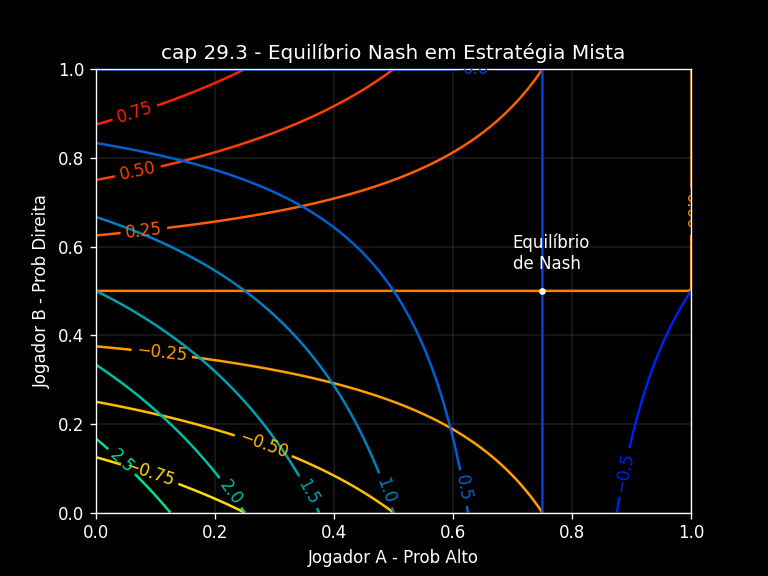
\includegraphics[scale=0.75]{cap29_3-estrategias_mistas.png}
\end{figure}

Como o professor afirma no livro. O ponto do equilíbrio de Nash acontece onde $B$ escolhe $50\%$ para cada e $A$ escolhe $75\%$ para $alto$ e $25\%$ para $baixo$. Quando $B$ escolhe esse ponto, todos os retornos de $A$ se tornam constantes (veja que a linha de $A$ é uma reta horizontal nesse ponto). Similarmente, quando $A$ escolhe esse ponto, todos os retornos de $B$ se tornam constantes. Como nenhum deles tem nenhum incentivo em mudar de estratégia nesse equilíbrio, temos um equilíbrio de Nash para estratégias mistas.\footnote{Eu sei, lindo demais, né?!}
\\
\\
\textbf{Comentário:} Aqui o professor coloca um exemplo muito bom sobre a relação entre teoria dos jogos e o jogo de pedra, papel e tesoura. Vale a pena a leitura.

\section{O Dilema do Prisioneiro}

Um dos conceitos mais conhecidos na economia é o dilema do prisioneiro. Chegou a sua hora de conhecê-lo. Primeiro, considere o jogo abaixo

\begin{center}

\def\sgtextcolor{white}% Trocar pra preto na versão white
\def\sglinecolor{white}% Trocar pra preto na versão white
\begin{game}{2}{2}[Jogador A][Jogador B]
            & $Confessa$      & $Nega$ \\
$Confessa$  & $-3,-3$         & $0,-6$ \\
$Nega$      & $-6,0$          & $-1,-1$
\end{game}

\end{center}

A essa altura você já notou que esse jogo possui uma estratégia dominante: confessar. Independente do que cada jogador faça, sempre vai ser melhor confessar. Mas aqui temos uma contradição. Se eles optassem por não seguir a estratégia dominante, acabariam em situação melhor.
\\
\\
Como a opção "nega-nega"\ não pode ser modificada sem prejuízo para alguma das parte, ela é eficiente no sentido de Pareto. Ou seja, estamos diante de um arranjo que impede que alcancemos o ótimo de Pareto do sistema.
\\
\\
Podemos adaptar esse dilema para várias outras situações da vida real. O professor cita uma adaptação para "instalar" ou "não instalar"\ um míssil. Também adapta esse jogo para a situação do cartel em que há as opões de "burlar" e "não burlar"\ as cotas de produção.
\\
\\
Como é de se esperar, o dilema do prisioneiro trouxe bastante discussão a respeito de como resolver esse jogo. Parece que a solução está relacionada à possibilidade ou não de repetição. Se o jogo é sem repetição, melhor será confessar. Pois essa é a estratégia dominante do arranjo.

\section{Jogos Repetidos}

Acabamos de falar sobre como a possibilidade de repetição pode modificar os resultados de um jogo. Dentro de um jogo repetido temos dois tipos: jogos de número fixo e jogos indefinidos.
\\
\\
Um jogo repetido pode permitir coordenações entre os jogadores. É possível "punir"\ um jogador que decida optar por um ponto egoísta e com isso, criar o incentivo à cooperação. No caso de um jogo com repetição fixa, é muito provável que os jogadores seguirão a estratégia dominante na última rodada, visto que não serão punidos pela outra parte. Acontece que essa lógica é refletida nas outras rodadas. Se você já sabe que o jogador será egoísta na última rodada, o que impede de ele repetir esse ato na penúltima, e na antepenúltima e assim por diante? Se não houver uma garantia de cooperação na última rodada, a maior chance é que o jogo siga na estratégia dominante.
\\
\\
Esse padrão não é mantido em um jogo indefinido. Como sempre haverá uma oportunidade de punir os comportamentos não cooperativos, a tendência é que os jogadores sigam para o equilíbrio de Pareto.
\\
\\
\textbf{Comentário:} Não está demarcado como exemplo, mas na página 744 o professor cita como o pesquisador Robert Axelrod fez um torneio computacional com vários algoritmos de estratégias em uma simulação do dilema do prisioneiro. A estratégia que performou melhor foi a que usou o "olho por olho". Leia a passagem no livro.

\section{Manutenção de um Cartel}

Nessa seção revisitamos o problema da manutenção do cartel, mas sob a ótica da teoria dos jogos. Na prática, esse problema pode ser modelo em termos de um dilema do prisioneiro onde seguir as cotas é igual ao ponto de cooperação e vender a custo competitivo (o ponto de Bertrand) é o equivalente a confessar e, portanto, é o equivalente ao equilíbrio de Nash.
\\
\\
\textbf{Comentário:} Depois ele cita o caso do Comitê Executivo Conjunto, que era um cartel gigante nos EUA no final do século XIX. Logo após ele coloca outro exemplo aplicando a teoria dos jogos ao problema de formação de preços das passagens aéreas. Vá ler o livro.

\section{Jogos Sequenciais}

Lá no capítulo do oligopólio nós vimos outros arranjos além dos jogos simultâneos. O modelo de Stackelberg é um exemplo de um jogo onde as ações são alternadas entre os jogadores. Nesses casos, além da matriz de ganhos, nós podemos usar a \textbf{forma extensiva do jogo} para ilustrar as etapas de escolhas e os devidos retornos de cada uma delas.
\\
\\
Observe o jogo abaixo

\begin{center}

\def\sgtextcolor{white}% Trocar pra preto na versão white
\def\sglinecolor{white}% Trocar pra preto na versão white
\begin{game}{2}{2}[Jogador A][Jogador B]
            & $Esquerda$     & $Direita$ \\
$Alto$      & $1,9$          & $1,9$ \\
$Baixo$     & $0,0$          & $2,1$
\end{game}

\end{center}

Se pensarmos nesse jogos como um jogo sequencial onde $A$ toma a primeira ação, podemos demonstrar o processo de decisão por meio do diagrama de árvore abaixo\footnote{Eu sei, eu sei. No livro está na horizontal. Mas o que importa é o conteúdo.}

\Tree[.\textit{Jogador A} 
				[.Alto 
					[.\textit{Jogador B}
						[.Esquerda (1,9) ]
						[.Direita (1,9) ]]]
				[.Baixo 
					[.\textit{Jogador B}
						[.Esquerda (0,0) ]
						[.Direita (2,1) ]]]]
\\
\ 
\\
Em uma primeira olhada na matriz de ganhos, poderíamos pensar que o jogo tínhamos dois equilíbrios de Nash. Mas quando colocamos o diagrama de árvore (ou a forma extensiva) podemos ver que o jogador $A$ tem como estratégia escolher $baixo$, pois assim, terá o retorno de $2$ ao invés de $1$. O jogador $B$ só tem a opção de escolher dentro das opções de $baixo$, o que lhe sobra é a opção $direita$.
\\
\\
Mas $B$ poderia pensar em manerias de obrigar o jogador $A$ a escolher $alto$. Se $B$ ameaçar uma retaliação e escolher $esquerda$, ambos terminariam com $0$. Contudo, $A$ só levaria a sério essa ameaça se houvesse forte indício de cumprimento. Uma maneira seria sinalizar por meio de um terceiro que se comprometesse a agir em desfavor dos dois caso o jogador $A$ optasse por $baixo$. Ou seja, se $B$ conseguir limitar seu escopo de atuação, é possível que a estratégia de $A$ seja modificada porque a matriz de ganhos seria modificada também.

\section{Um jogo com Barreiras à Entrada}

Voltemos no problema da entrada de concorrentes em um mercado monopolizado. Nós vimos que o monopolista possui o poder de retalhar devido a escala mínima de eficiência (EME) e do controle do mercado. Quando uma empresa pondera em entrar no mercado, ela precisa contar com as possíveis consequências por conta do monopolista e, da mesma maneira, o monopolista precisa ponderar se valerá a pena baixar os preços para evitar o concorrente.
\\
\\
Podemos exemplificar essa questão com a matriz abaixo

\begin{center}

\def\sgtextcolor{white}% Trocar pra preto na versão white
\def\sglinecolor{white}% Trocar pra preto na versão white
\begin{game}{2}{2}[Entrante][Monopolista]
                      & $Retalha$      & $\textrm{Não Retalha}$ \\
$Entra$               & $0,0$          & $2,1$ \\
$\textrm{Fica Fora}$  & $1,9$          & $1,9$
\end{game}

\end{center}


A primeira vista, temos dois equilíbrios de Nash. Mas esse também é um exemplo de um jogo sequenciado. Quem tem o poder de liderança é a empresa entrante.

\Tree[.\textit{Entrante} 
				[.\textit{Fica Fora} 
					[.\textit{Monopolista}
						[.Retalha (1,9) ]
						[.\textit{Não Retalha} (1,9) ]]]
				[.Entra
					[.\textit{Monopolista}
						[.Retalha (0,0) ]
						[.\textit{Não Retalha} (2,1) ]]]]
\\
\ 
\\
Como podemos ver, a condição de entrada ou não é baseada na promessa de haver ou não retalhação. Esse esquema é igual ao que acabamos de ver na última seção. A estratégia da entrante é optar por concorrer no mercado. O que o monopolista fará? Bom, não existe maneira garantida do monopolista vincular a entrada do novo concorrente com a retaliação. Uma vez que o novo competidor se instalou, não é racional baixar os preços e abrir mão do lucro.
\\
\\
Agora, se o monopolista conseguir modificar sua matriz de ganhos (por meio de investimento na capacidade produtiva) de modo a obter lucro mesmo na retalhação, o cenário será outro. Se a árvore de decisão fosse igual a 

\Tree[.\textit{Entrante} 
				[.\textit{Fica Fora} 
					[.\textit{Monopolista}
						[.Retalha (1,9) ]
						[.\textit{Não Retalha} (1,9) ]]]
				[.Entra
					[.\textit{Monopolista}
						[.Retalha (0,2) ]
						[.\textit{Não Retalha} (2,1) ]]]]
\\
\ 
\\
Seria mais compensador ao monopolista lutar pelo seu mercado do que se acovardar. Nesse novo arranjo, o melhor a fazer é ficar de fora do mercado. O interessante é que o investimento feito na capacidade produtiva ficará ocioso, mas ainda assim, para o monopolista é vantajoso ter essa capacidade de barganha oriunda do excesso de capacidade produtiva.

%%%%%%%%%%%%%%%%%%%%%%%% CHAPTER %%%%%%%%%%%%%%%%%%%%%%%%
\chapter{Aplicações da Teoria dos Jogos}

Ainda nos ateremos à teoria dos jogos nesse capítulo. Aqui vamos aprender um ferramental novo para analisar os equilíbrios dos jogos, bem como veremos alguns modelos mais avançados de jogos.

\section{Curvas de Melhor Resposta}

Analise o jogo abaixo

\begin{center}

\def\sgtextcolor{white}% Trocar pra preto na versão white
\def\sglinecolor{white}% Trocar pra preto na versão white
\begin{game}{2}{2}[Linha][Coluna]
         & $Esquerda$     & $Direita$ \\
$Alto$   & $2,1$          & $0,0$ \\
$Baixo$  & $0,0$          & $1,2$
\end{game}

\end{center}

Podemos ver que não temos uma estratégia dominante, mas temos dois equilíbrios de Nash. Chamaremos de \textbf{melhor resposta} àquelas escolhas que os jogadores fizerem que maximizem seus retornos. Se existirem mais de uma escolhas maximizadoras, então a melhor resposta será um conjunto desses escolhas.
\\
\\
Agora vamos formalizar um pouco mais essas ideias. Seja um jogo com dois jogadores. O jogador linha terá $l_1,l_2,\dots,\l_L$ escolhas, similarmente, o jogador coluna terá $c_1,c_2,\dots,c_C$ opções de escolhas.
\\
\\
Para cada escolha $l$ feita, chamaremos de $b_c(l)$ a melhor escolha para coluna dada a escolha de linha. Da mesma maneira, chamaremos $b_l(c)$ a melhor escolha para linha. Um equilíbrio de Nash será o par de estratégias $(l^*,c^*)$ tal que

\newpage

$$ c^* = b_c(l^*) $$
$$ l^* = b_l(c^*) $$

Eu já tinha adiantado a formalização lá no ponto 29.3. Mas não custa nada repetir o conceito. Veja com o equilíbrio de Nash é consistente. É um arranjo cuja estratégia de um é precisamente dependente da estratégia do outro, de modo a manter esse ciclo de reforço mútuo.
\\
\\
Já vimos situações onde algum jogador pode ser indiferente ao retorno dada alguma escolha do outro jogador. É o caso onde só é benéfico para um deles, enquanto o outro terá o mesmo resultado independente da escolha. Mas isso não é um problema, os pontos $c^*$ e $l_*$ só precisar ser uma da melhores respostas.\footnote{É o caso dos jogos com mais de um equilíbrio do Nash}. Se existir apenas uma melhor resposta, então poderemos representar o equilíbrio por meio de uma \textbf{função de melhor resposta}.
\\
\\
Os equilíbrios de Cournout e Bertrand são exemplos de jogos com equilíbrios de Nash. No "jogos"\ de definir a quantidade e o preço, as empresas acabam adotando a posição de produzir nos pontos de maximização de lucro, em função do que  esperam que suas concorrentes irão fazer. Isso as leva a produzir exatamente no ponto onde as curvas de reação se encontram e o equilíbrio é reforçado.

\section{Estratégias Mistas}

Voltaremos ao jogo da seção anterior

\begin{center}

\def\sgtextcolor{white}% Trocar pra preto na versão white
\def\sglinecolor{white}% Trocar pra preto na versão white
\begin{game}{2}{2}[Linha][Coluna]
         & $Esquerda$     & $Direita$ \\
$Alto$   & $2,1$          & $0,0$ \\
$Baixo$  & $0,0$          & $1,2$
\end{game}

\end{center}

Mas dessa vez, nosso interesse é no equilíbrio de estratégias mistas e, também, nos de estratégias puras. Já aprendemos que uma estratégia mista consiste na escolha das probabilidades para cada ação, de modo a obter os retornos proporcionais à cada probabilidade atribuída. Os jogos de estratégia pura podem ser explicados pelo mesmo modelo, só que com probabilidades iguais aos extremos (0\% e 100\%).
\\
\\
Primeiro vamos equacionar os retornos em termos das probabilidades de cada escolha. As probabilidades do jogador $linha$ serão: $l$ para $alto$ e $(1-l)$ para $baixo$. Do mesmo modo, para o jogador $coluna$ teremos: $c$ para $esquerda$ e $(1-c)$ para $direita$.
\\
\\
As probabilidades e os ganhos para o jogador $linha$ para cada combinação serão:

\begin{center}

\def\sgtextcolor{white}% Trocar pra preto na versão white
\def\sglinecolor{white}% Trocar pra preto na versão white
\begin{game}{2}{2}[Linha][Coluna]
         & $Esquerda$     & $Direita$ \\
$Alto$   & $lc = 2$       & $l(1-c) = 0$ \\
$Baixo$  & $(1-l)c = 0$   & $(1-l)(1-c) = 1$
\end{game}

\end{center}

O resultado do jogador $linha$ é obtido pela soma de cada probabilidades ponderada pelo retorno em cada quadrante. No caso da linha $alto$ temos

$$ \textrm{ganhos linha} = 2lc + 0(l(1-c)) + 0((1-l)c) + (1-l)(1-c) $$
$$  = 2lc + (1-l)(1-c) $$
$$  = 2lc + 1 - l - c + lc $$

Chegamos em um lugar bem interessante, temos uma função que relaciona as probabilidades de cada estratégia ($l$, $(1-l)$, $c$ e $(1-c)$) a cada nível de retorno para o jogador $linha$. Podemos ver o quanto uma variação na probabilidade que ele tem controle $\Delta l$ pode trazer de retorno

$$ \frac{d \textrm{ (ganhos linha)}}{d l} = 2c - 1 + c $$
$$ = 3c - 1 $$

Com esse resultado, podemos ver que, se  $c > 1/3$ qualquer aumento em $l$ gerará um resultado positivo. Por outro lado, se $c < 1/3$ qualquer valor de $l$ positivo terá um retorno negativo (nesse caso, ele escolhe não jogar $alto$). Por fim, se $c = 1/3$, não importa o que o jogador $linha$ faça, seus retornos serão constantes.
\\
\\
De maneira análoga, podemos ver que as probabilidades e os ganhos do jogador $coluna$ são iguais a 

\begin{center}

\def\sgtextcolor{white}% Trocar pra preto na versão white
\def\sglinecolor{white}% Trocar pra preto na versão white
\begin{game}{2}{2}[Linha][Coluna]
         & $Esquerda$     & $Direita$ \\
$Alto$   & $lc = 1$       & $l(1-c) = 0$ \\
$Baixo$  & $(1-l)c = 0$   & $(1-l)(1-c) = 2$
\end{game}

\end{center}

Fazendo a mesma análise a partir desses valores, podemos ver que

$$ \textrm{ganhos coluna} = lc + 0(l(1-c)) + 0((1-l)c) + 2(1-l)(1-c) $$
$$  = lc + 2(1-l)(1-c) $$
$$  = lc + 2(1-l-c+lc) $$
$$  = lc + 2 - 2l - 2c + 2lc $$
$$  = 3lc + 2 - 2l - 2c $$

Cuja derivada em relação à $c$ será

$$ \frac{d \textrm{ (ganhos coluna)}}{d c} =  $$
$$ = 3l - 2 $$

Podemos concluir que, quando $l < 2/3$, qualquer ação de $c$ levará a uma redução no seu resultado (esse é o caso onde é melhor não fazer nada de $esquerda$). Se $l > 2/3$, qualquer aumento de $c$ elevará o seu resultado. Finalmente, se $l = 2/3$, qualquer valor de $c$ terá retornos constantes.
\\
\\
Com base nessas informações, podemos construir as curvas de melhor resposta no gráfico abaixo.

\begin{figure}[H]
\centering
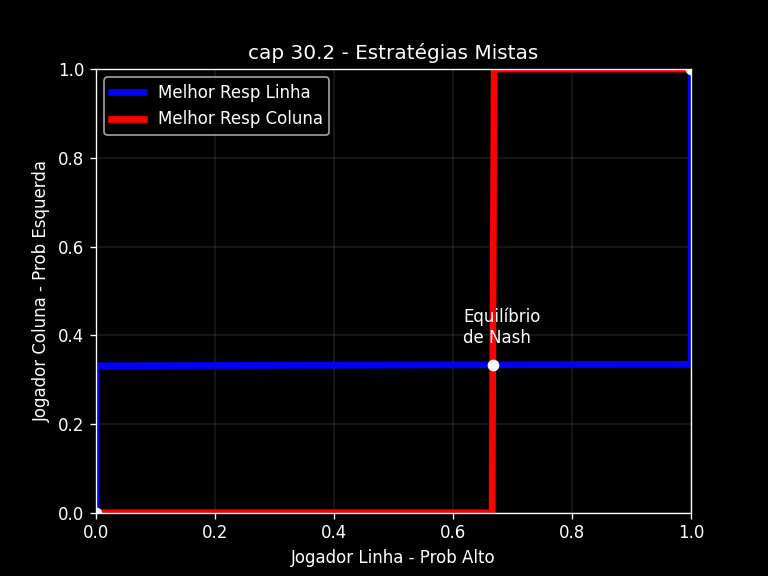
\includegraphics[scale=0.75]{cap30_2-estrategias_mistas.png}
\end{figure}

Podemos ver que temos 3 equilíbrios de Nash. Dois em estratégias puras: o ponto $(0,0)$ e o ponto $(1,1)$. E também um equilíbrio em estratégia mista: o ponto $(2/3,1/3)$.

\section{Jogos de Coordenação}

De posse das curvas de melhor resposta, vamos começar a investigar algumas classes de jogos. A primeira que veremos são os \textbf{jogos de coordenação}. Que são jogos onde os ganhos serão maiores se os jogadores decidirem coordenar suas estratégias. A questão é criar os mecanismos que criem os incentivos à essa coordenação.

\subsection{A Batalha dos Sexos}

Imagine que temos dois jovens enamorados. Ambos marcaram que iriam se encontrar no cinema, mas estão sem celular\footnote{O do rapaz foi roubado e o da moça está sem bateria.} e não sabem qual filme o outro verá. O rapaz prefere o filme de ação enquanto a moça prefere o filme de arte. Ambos preferem assistir a algum filme juntos do que não se encontrarem. Podemos traduzir essa estrutura em uma matriz de ganhos

\begin{center}

\def\sgtextcolor{white}% Trocar pra preto na versão white
\def\sglinecolor{white}% Trocar pra preto na versão white
\begin{game}{2}{2}[Rapaz][Moça]
         & $Ação$     & $Arte$ \\
$Ação$   & $2,1$      & $0,0$ \\
$Arte$   & $0,0$       & $1,2$
\end{game}

\end{center}

Já sabemos que essa matriz produz as curvas de melhor resposta vistas na seção passada. Então esse jogo tem 3 equilíbrios. Nos dois equilíbrios de estratégia pura, teremos as opções: Ambos arriscam se encontrar no filme de Ação, Ambos arriscam se encontrar no filme de Artes. No equilíbrio de estratégia mista, cada um arriscaria no seu filme preferido com $2/3$ de probabilidade\footnote{Outra maneira é pensar que cada um ficaria $2/3$ do tempo na entrada do seu filme preferido}.
\\
\\
Da maneira como está descrito, não tem como a gente saber o resultado dessa história. Se supormos que o rapaz tenha o histórico de ceder as decisões para a moça\footnote{Uma hipótese não muito rara na realidade.}, podemos definir que esse jogo teria um equilíbrio "mais natural"\ que os outros. O termo comumente usado para essa diferenciação dos equilíbrios é \textbf{ponto focal} do jogo.

\subsection{O Dilema do Prisioneiro}

Esse você já deve estar enjoado de ver. Mas agora temos as curvas de melhor resposta para ajudar na nossa análise\footnote{Não que isso vá mudar as conclusões que já temos.}. Sabemos que a estratégia dominante é confessar. Mas também sabemos que a estratégia eficiente no sentido de Pareto é negar.

\begin{center}

\def\sgtextcolor{white}% Trocar pra preto na versão white
\def\sglinecolor{white}% Trocar pra preto na versão white
\begin{game}{2}{2}[Jogador A][Jogador B]
            & $Confessa$      & $Nega$ \\
$Confessa$  & $-3,-3$         & $0,-6$ \\
$Nega$      & $-6,0$          & $-1,-1$
\end{game}

\end{center}

Quando modelamos as funções de melhor resposta. Como já sabemos, a única estratégia de equilíbrio é no ponto "confessa-confessa". No resto da seção não tem muita informação nova. Mas você tem que ler.

\begin{figure}[H]
\centering
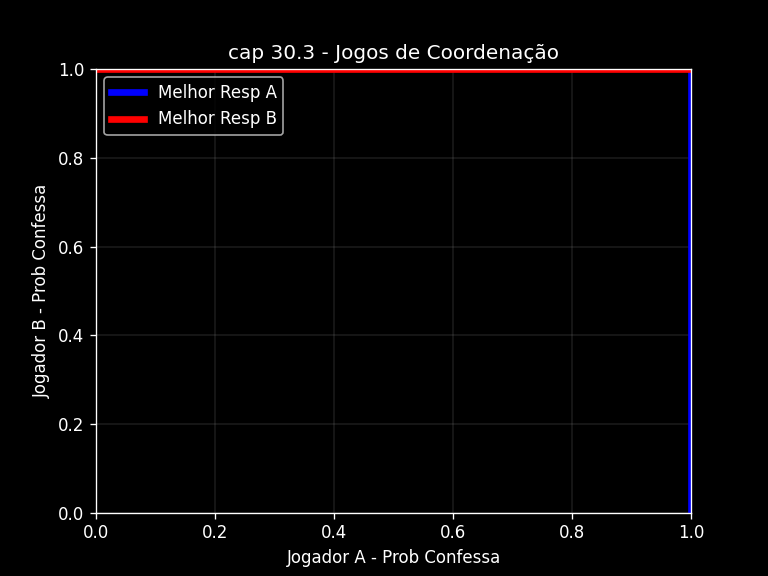
\includegraphics[scale=0.75]{cap30_3-jogos_coordenacao_1.png}
\end{figure}

\subsection{Jogos de Garantia}

Uma coisa bacana da teoria dos jogos, é que podemos aplicar para uma gama enorme de contextos. Pensemos na corrida amarmentista de meados do século XX. Todo mundo sabe que o melhor era optar por não construir mais mísseis nucleares. Mas o custo de ser surpreendido por uma trapaça do outro lado\footnote{"Malditos comunistas!", diriam eles.}. Podemos resumir esse cenário na tabela abaixo

\begin{center}

\def\sgtextcolor{white}% Trocar pra preto na versão white
\def\sglinecolor{white}% Trocar pra preto na versão white
\begin{game}{2}{2}[EUA][URSS]
            & $Abstém$      & $Constrói$ \\
$Abstém$    & $4,4$         & $1,3$ \\
$Constrói$  & $3,1$         & $2,2$
\end{game}

\end{center}

O gráfico das curvas de melhor resposta é esse aqui.

\begin{figure}[H]
\centering
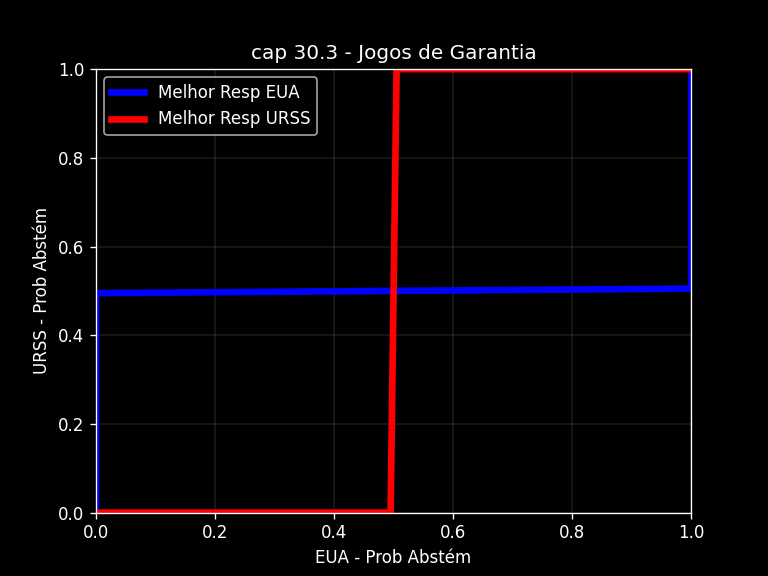
\includegraphics[scale=0.75]{cap30_3-jogos_coordenacao_2.png}
\end{figure}

Vemos que, como esse jogo é simultâneo, não temos uma estratégia mista. Nesse caso, só temos os pontos de equilíbrio nos extremos. Se um dos participantes conseguir convencer o outro que se abstém, ele "empurrará"\ o outro jogador para o ponto de equilíbrio da abstenção. A questão toda era como sinalizar de maneira eficiente para o outro jogador e ainda não parecer que está desistindo da corrida.

\subsection{Roleta Russa}

Antigamente, era comum ver, nos \href{https://www.youtube.com/watch?v=u7hZ9jKrwvo}{filmes de adolescentes americanos}\footnote{Nesse link tem uma versão um pouco diferente do jogo, mas a lógica é a mesma. (Embora o carinha tenha roubado ao pular do carro).}, uma prática chamada "roleta russa"\ que consistia em dois veículos um de frente para o outro à uma distância considerável. Os veículos aceleravam em direção ao outro. A ideia é que o motorista mais corajoso não desviaria a trajetória\footnote{A um lista de microeconomia pra essa garotada arranjar o que fazer!}. A matriz de ganhos pode ser definida como

\begin{center}

\def\sgtextcolor{white}% Trocar pra preto na versão white
\def\sglinecolor{white}% Trocar pra preto na versão white
\begin{game}{2}{2}[Linha][Coluna]
           & $Desvia$    & $Mantém$ \\
$Desvia$   & $0,0$       & $-1,1$ \\
$Mantém$   & $1,-1$      & $-2,-2$
\end{game}

\end{center}

Diferente dos outros jogos, aqui os equilíbrios são nas opções contrárias. Os equilíbrios de Nash de estratégia pura estão nas opções onde eles seguem ações diferentes.

\begin{figure}[H]
\centering
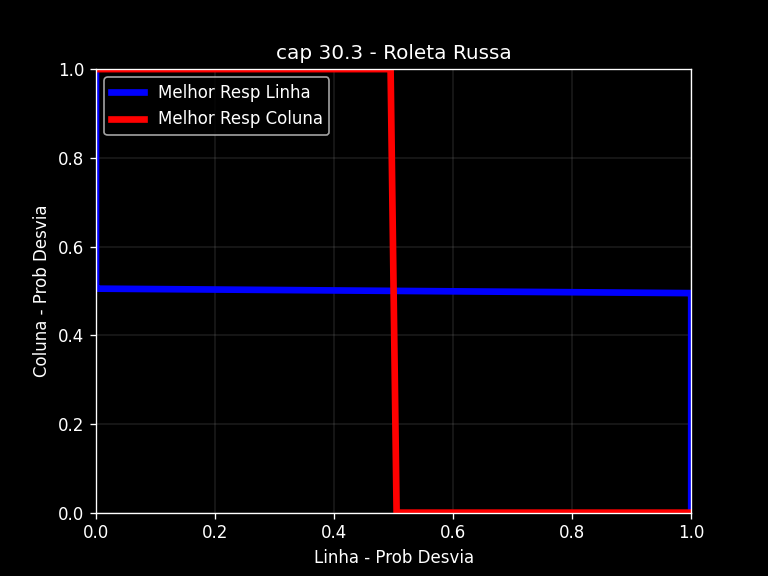
\includegraphics[scale=0.75]{cap30_3-jogos_coordenacao_3.png}
\end{figure}

Como encontrar um resultado? Bom, a melhor maneira de encontrar um desfecho é pela sinalização de compromisso. Se um dos competidores arrancasse fora o volante, ele jogaria para o outro motorista toda a responsabilidade pelo resultado. Nesse caso, a matriz seria atualizada e seria melhor para o outro motorista sair derrotado do que bater o carro.

\subsection{Como Coordenar?}

Essa seção é bem pequeninha. Vá ler o original. Mas um resumo é que podemos modificar os resultados pela adoção de movimentos sequenciados, repetição ou contratação.
\\
\\
Quando modificamos os jogos da segurança, batalha dos sexos e roleta russa, para jogos sequenciados. Quando um jogado faz o primeiro movimento, o outro terá que maximizar apenas a partir do movimento feito. No caso da roleta russa, isso daria a vitória a um delas. Nos outros jogos, isso levaria ao ponto eficiente de Pareto.
\\
\\
No caso do dilema do prisioneiro, o melhor a fazer seria modificar o jogo para repetição (que permitiria a retalhação por mal comportamento) ou a contratação (que modificaria o resultado da confissão). 

\section{Jogos de Competição}

O contrário do jogo de coordenação é a competição. Você já ouviu falar que "tal coisa é um \textbf{jogo de soma zero}". Bem, esse nome é devido ao fato que o total de ganhos é igual ao as perdas. Os esportes são um bom exemplo desse tipo de arranjo.
\\
\\
Considere essa matriz para pontuação de um pênalti

\begin{center}

\def\sgtextcolor{white}% Trocar pra preto na versão white
\def\sglinecolor{white}% Trocar pra preto na versão white
\begin{game}{2}{2}[Artilheiro][Goleiro]
             & $Esquerda$    & $Direita$ \\
$Esquerda$   & $50,-50$      & $80,-80$ \\
$Direita$    & $90,-90$      & $20,-20$
\end{game}

\end{center}

Os valores são variáveis porque simbolizam as probabilidades de gol. Como o goleiro quer defender, e o artilheiro quer marcar. Eles farão de tudo para impedir que um saiba de antemão a ação do outro. Esse é um baita exemplo de uma \textbf{estratégia mista}.
\\
\\
Como esse jogo é competitivo, não teremos opções de equilíbrio em estratégia pura cooperativos. Graficamente, isso quer dizer que as curvas de melhor resposta não se encontrarão em nenhum extremo do gráfico.
\\
\\
Quando o artilheiro escolhe chutar para esquerda com prob. igual a $p$. O seu retorno esperado será de $50p + 90(1-p)$ caso o goleiro pule para a esquerda, mas caso o goleiro pule para a direita, seu retorno será de $80p + 20(1-p)$. O artilheiro quer ter o maior retorno possível com seus chutes, enquanto o goleiro quer que seja o menor possível.
\\
\\
Se o artilheiro decidir chutar mais para uma direção, ou optar pela metade em cada, o goleiro utilizará as probabilidades de defesa para fazer sua estratégia de maximização. A única maneira que o artilheiro tem de "obrigar"\ o goleiro a adotar determinada conduta, é optar pelo ponto onde os retornos prováveis serão iguais. Nós conseguimos saber esse ponto pela igualdade das duas curvas de retorno.

$$50p + 90(1-p) = 80p + 20(1-p)$$
$$70(1-p) = 30p$$
$$70 - 70p = 30p$$
$$70 = 100p$$
$$p = 0,7$$

Ao adotar a estratégia de chutar 70\% das vezes para a esquerda, o artilheiro se coloca em uma situação os retornos esperados são iguais nos acertos ou nos erros. É a melhor estratégia a ser tomada pois, "anula"\ o efeito que o goleiro possa fazer no resultado.
\\
\\
Se fizermos exatamente a mesma abordagem para o goleiro, acabaremos com

$$50q + 80(1-q) = 90q + 20(1-q)$$
$$60(1-q) = 40q$$
$$60 - 60q = 40q$$
$$60 = 100q$$
$$q = 0,6$$

Esse será o ponto onde o goleiro obterá retornos constantes, independente da escolha do artilheiro.
\\
\\
Agora podemos construir o gráfico com as curvas de melhor resposta. Sabemos que o equilíbrio de Nash acontecerá no ponto $p = 0,7$ e $q = 0,6$.

\begin{figure}[H]
\centering
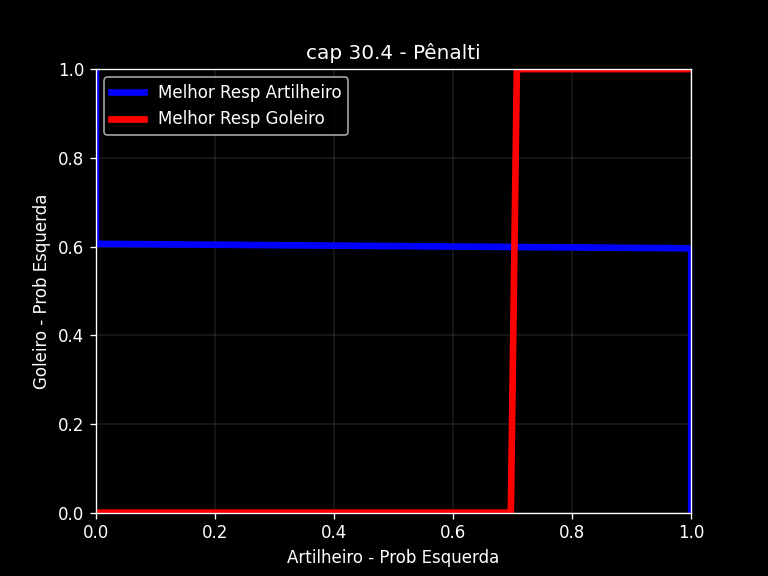
\includegraphics[scale=0.75]{cap30_4-jogos_competitivos.png}
\end{figure}

\section{Jogos de Coexistência}

Agora veremos a teoria dos jogos em um contexto natural. Imagine que exista uma espécie de cachorro selvagem. Se dois animais encontram um pedaço de comida, eles têm de decidir entre brigar ou dividir. O nome dessa interação é \textbf{jogo de pombos e falcões}\footnote{Ficou curioso com o nome né? Essa eu deixo pra você pesquisar por conta própria.}. A matriz dos ganhos está abaixo

\begin{center}

\def\sgtextcolor{white}% Trocar pra preto na versão white
\def\sglinecolor{white}% Trocar pra preto na versão white
\begin{game}{2}{2}[Animal linha][Animal coluna]
           & $Lutar$    & $Dividir$ \\
$Lutar$    & $-2,-2$    & $4,0$ \\
$Dividir$  & $0,4$      & $2,2$
\end{game}

\end{center}

Esse caso é muito interessante. Veja que nenhum dos quadrantes iguais é estável. Se ambos lutarem, é melhor abrir mão do que sair ferido. Se ambos dividirem, é melhor atacar para ficar com tudo.
\\
\\
Aqui vai uma adaptação interessantíssima dessa teoria. Ao invés de pensarmos em apenas dois animais com escolhas variáveis ao longo do tempo, podemos supor que temos um grupo de animais que se comportarão de maneira diferente. Nesse modelo, as probabilidades fazem jus a quantidade esperada de cada grupo de animais em cada interação.
\\
\\
A probabilidade de algum animal lutar será dada por $p$, assim, a chance de um lutador encontrar outro é de $p$ e de encontrar um disposto a dividir será igual a $1 - p$.
\\
\\
O ganho esperado para os lutadores será de

$$H = -2p + 4(1-p)$$

Enquanto o ganhos dos que dividirão

$$D = 2(1-p)$$

Como estamos falando de animais, as estratégias de maior retorno produzirão indivíduos mais capazes de se reproduzir. Supondo que as características sejam transferidas, o grupo com o maior retorno terá a maior chance de ser encontrado. Se $H > D$, então veremos a população dos brigões aumentar. Caso $D > H$, então, a população de cooperadores aumentará.
\\
\\
O equilíbrio entre essas populações será dado pela igualdade

$$H -2p + 4(1-p) = 2(1-p) = D$$
$$2(1-p) = 2p$$
$$2 - 2p = 2p$$
$$p = 1/2$$

Agora vamos ver como se comportam as curvas de melhor resposta.

\begin{figure}[H]
\centering
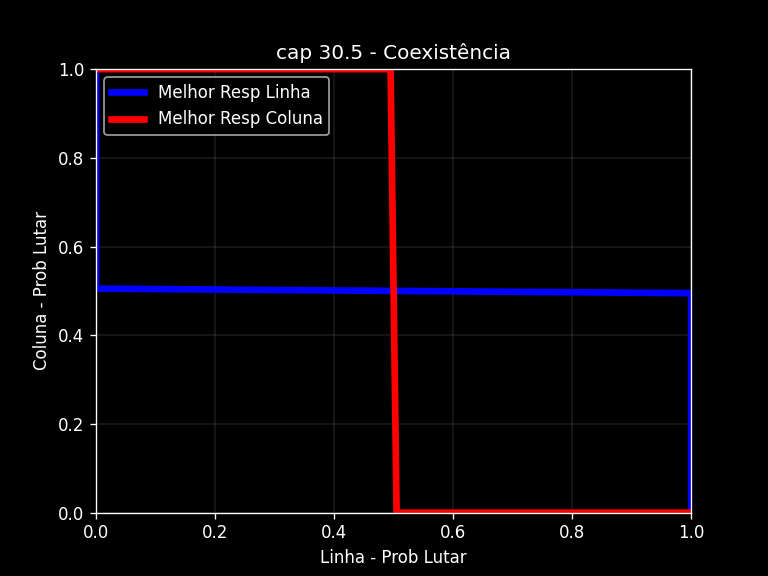
\includegraphics[scale=0.75]{cap30_5-coexistencia_1.png}
\end{figure}

Aqui vemos 3 condições de equilíbrio. Mas nosso equilíbrio não foi alcançado no ponto $1/2$? A resposta é sim. Perceba que os pontos de estratégia dominante são os pontos onde há o incentivo de se jogar o oposto do adversário\footnote{Igual o caso da roleta russa}. Mas esse jogo não lida com apenas 2 agentes e sim com uma população homogênea com duas opções de comportamento. O único ponto onde as estratégias convergem é o ponto $1/2$.
\\
\\
Por causa da estabilidade desse arranjo, os pesquisadores o classificam como uma \textbf{estratégia evolucionariamente estável}. É pura teoria dos jogos e vem diretamente dos estudos das dinâmicas entre interações animais.
\\
\\
Assim como está no livro, eu coloquei os resultados para cada estratégia a medida que o número de lutadores aumenta de $0$ até $100\%$.

\begin{figure}[H]
\centering
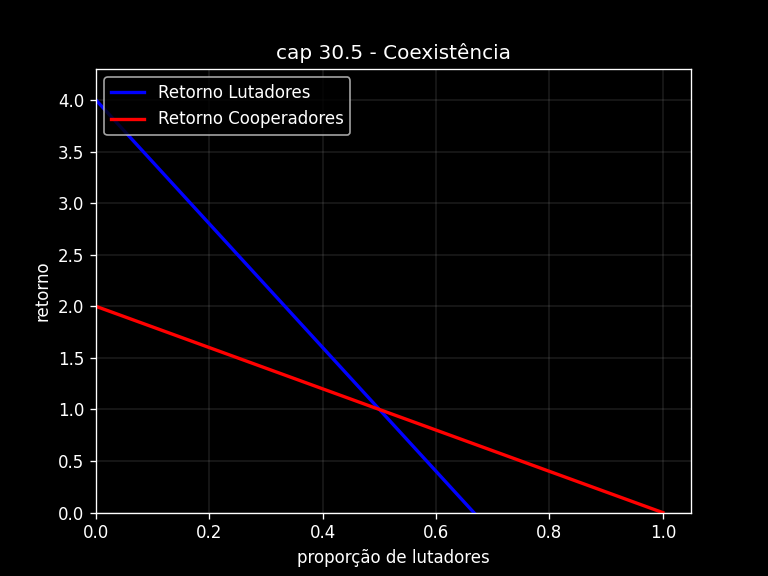
\includegraphics[scale=0.75]{cap30_5-coexistencia_2.png}
\end{figure}

Como podemos ver, para todos os pontos abaixo de $1/2$, vale mais a pena se lutador. Acima desse ponto, é melhor cooperar. Os retornos se equivalem no ponto de equilíbrio.

\section{Jogos de Compromisso}

Os jogos que vimos até agora são do jogos \textbf{com movimentos simultâneos}. Os jogadores não sabem o que o outro fará, e precisam maximizar de acordo com a suposição do comportamento do adversário.
\\
\\
Aqui vamos ver os jogos com \textbf{movimento sequenciais}. Um conceito importante nesses jogos é o \textbf{compromisso}. Quando um participante se compromete a agir de terminada maneira ele precisa garantir: 1) que ele não terá outro caminho a seguir além do firmado anteriormente; 2) que a sinalização do compromisso chegue ao outro jogador e seja entendida por ele.

\subsection{O Sapo e o Escorpião}

Você já deve conhecer essa história. Então vamos pular direto para a modelagem em termos da teoria dos jogos. Podemos recriar a situação da fábula como o seguinte jogo sequencial

\Tree[.\textit{Sapo}
				[.Carrega 
					[.Escorpião 
						[.Ferroada $(-10,5)$ ]
						[.\textit{Não Ferroada} $(5,3)$ ]]]
				[.\textit{Não Carrega} $(0,0)$ ]]
\\
\ 
\\
Mesmo que a moral da história seja nós ensinar que existem pessoas que preferem fazer o mal. Sob a ótica da teoria dos jogos, o escorpião apenas maximizou sua utilidade dada as opções disponíveis. Como o sapo escolheu antes, só restou ao escorpião entre ter $5$ de retorno com a ferroada ou $3$ com o passeio.
\\
\\
Se o sapo tivesse a oportunidade de estudar esse material, ele se certificaria em reduzir o resultado do escorpião na opção da ferroada. Como o escorpião é meio suicida, talvez uma solução fosse o sapo falar sobre como é bom estar vivo. Ele também poderia ameaçar que os outros sapos fariam uma retalhação aos outros escorpiões. Ou mesmo propor que a cauda do passageiro fosse amarrada antes do transporte. Não importa como, o que o sapo deveria ter feito é tornar o retorno da não ferroada maior que o da ferroada.

\Tree[.\textit{Sapo}
				[.Carrega 
					[.Escorpião 
						[.Ferroada $(-10,2)$ ]
						[.\textit{Não Ferroada} $(5,3)$ ]]]
				[.\textit{Não Carrega} $(0,0)$ ]]
\\
\ 
\\
Nesse jogo, todos chegariam ao lado do rio e a moral da história seria como é bom ajudar os outros independente da aparência deles.

\subsection{O Sequestrador Cordial}

É isso mesmo, nós vamos modelar o comportamento de um grupo de sequestradores. A Economia é ou não é uma ciência cheia de surpresas? Pois bem, imagine que um CEO de uma empresa é sequestrado. No regimento interno da empresa está a cláusula de não pagamento de resgate em caso de sequestro dos seus funcionários (mesmo os da cúpula). O que os sequestradores farão? Uma possibilidade de arranjo é esse abaixo

\Tree[.\textit{Sequestradores}
				[.Libera 
					[.Refém 
						[.Identifica $(-5,5)$ ]
						[.\textit{Não Identifica} $(5,3)$ ]]]
				[.\textit{Mata} $(-3,-10)$ ]]
\\
\ 
\\
O resultado desse jogo é inteiramente dependente da capacidade do refém de sinalizar para os sequestradores que cumprirá seu lado do trato em não identificar. Uma saída para esse impasse é a proposta pelo pesquisador Thomas Schelling. Eu não vou estragar a surpresa, leia a (inusitada) proposta de solução no material original.

\subsection{Quando Força é Fraqueza}

A psicologia animal\footnote{Sim, eu também não fazia ideia que existia esse campo de pesquisa.} também fez algumas incursões na teoria dos jogos. Eles perceberam que num grupo, os porcos rapidamente desenvolvem uma relação de dominação em relação ao porco dominador.
\\
\\
Eles colocaram uma alavanca em uma lado da baia que, quando acionada, fazia com que o alimento caísse do outro lado da baia. Como o porco dominador não tem como evitar que o subordinado coma, nem consegue obrigá-lo a puxar, ao se negar a puxar a alavanca, o porco subordinado condena o dominador a comer os seus restos.

\begin{center}

\def\sgtextcolor{white}% Trocar pra preto na versão white
\def\sglinecolor{white}% Trocar pra preto na versão white
\begin{game}{2}{2}[Subordinado][Dominador]
                      & $Puxar$    & $\textrm{Não Puxar}$ \\
$Puxar$               & $0,0$      & $4,1$ \\
$\textrm{Não Puxar}$  & $0,5$      & $2,3$
\end{game}

\end{center}

A estratégia do porco subordinado é sempre esperar pela comida. Enquanto o dominador não tem outra opção a não ser aceitar os restos.

\subsection{Poupanças e Seguridade Social}

Mais um jogo para analisarmos. Agora vamos aplicar nossos conceitos ao modelos de seguridade social. Podemos modelar esse jogo como uma relação entre gerações do seguinte modo

\begin{center}

\def\sgtextcolor{white}% Trocar pra preto na versão white
\def\sglinecolor{white}% Trocar pra preto na versão white
\begin{game}{2}{2}[+ Velhos][+ Jovens]
           & $Sustenta$ & $Poupa$ \\
$Poupa$    & $2,-1$      & $1,0$ \\
$Esbanja$  & $3,-1$      & $-2,-2$
\end{game}

\end{center}

Da pra ver que temos dois equilíbrios ai. Um no ponto onde os velhos poupam e os jovens também poupam. O outro é no ponto onde os velhos esbanjam e os jovens sustentam. Mas esse jogo tem um caráter temporal mais do que evidente, uma vez que é claro que os velhos terão prioridade na escolha da ação.

\Tree[.\textit{Velhos}
				[.Poupam 
					[.Jovens 
						[.Sustentam $(2,-1)$ ]
						[.Poupam $(1,0)$ ]]]
				[.Esbajam
					[.Jovens 
						[.Sustentam $(3,-1)$ ]
						[.Poupam $(-2,-2)$ ]]]]
\\
\ 
\\
Conseguimos ver que a melhore estratégia para os velhos é usar o poder da preferência e escolher esbanjar. Os jovens serão obrigados a optar por sustentá-los. Mas não é atoa que a maioria dos países possui algum programa em que cada geração acaba contribuindo para o montante da sua aposentadoria.
\\
\\
\textbf{Comentário:} Aqui o professor coloca um exemplo da discriminação de preço à luz da teoria dos jogos.

\subsection{Extorsão}

Estamos na última subseção. Aquente firme. O problema que veremos aqui é bem comum e pode se adaptar a várias situações parecidas. Imagine uma obra chegando ao final. Se o cliente quiser alterar alguma coisa nessa reta final, o empreiteiro poderá tirar alguma vantagem disso? Considere a árvore abaixo

\Tree[.\textit{Empreiteiro}
				[.Extorque 
					[.Cliente 
						[.Paga $(1.300,0)$ ]
						[.\textit{Não Paga} $(0,-100)$ ]]]
				[.\textit{Não Extorque} $(0,1.300)$ ]]
\\
\ 
\\
Como podemos ver, o empreiteiro tem todo o incentivo em usar o poder de extorsão para faturar a mais. Uma maneira que o cliente poderia se proteger é por via contratual ou ameaçar fazer propaganda negativa como forma de retalhação.

\section{Negociação}

Nessa última parte do capítulo, pensemos em um problema simples: a divisão de um dólar entre duas pessoas. Como faríamos de modo a satisfazer a vontade de ambas? O foco está em construir uma solução que permita a negociação.
\\
\\
O \textbf{modelo de negociação de Nash}, usa uma abordagem a partir de proposições a respeito do comportamento dos indivíduos. O livro não entra muito no modelo, mas como eu sou curioso, eu vou colocar um pouco mais de informação sobre ele. Os axiomas usados são

\begin{itemize}
\item Eficiência de Pareto
\item Simetria na Solução
\item Invariância das Representações Equivalentes dos Resultados
\item Independência das Alternativas Irrelevantes
\end{itemize}

O modelo de negociação de Nash é o modelo que resolver o problema de maximização do tipo

\begin{center}
\LARGE $\stackrel{máx}{\text{\small $v_1,v_2$}} \ \ \stackrel{(v_1 - d_1)(v_2 - d_2)}{\ }$ \\
\normalsize Sujeito a $(v_1,v_2) \in U$ e $(v_1,v_2) \geq (d_1,d_2)$
\end{center}

Nash demonstrou que existe uma solução desse problema, denotada por $f^N(U,d)$, e que essa solução é única. Mas esse tipo de conteúdo é material de pós-graduação.
\\
\\
Uma outra abordagem é o \textbf{modelo de negociação de Rubinstein}. Esse modelo o livro explica um pouco mais. Imaginemos dois jogadores, A e B, que precisam dividir um dólar entre eles. Terão 3 dias para decidir. A faz uma proposta, B pode aceitar, ou voltar no outro dia com uma contraproposta. Se A não aceitar, poderá fazer uma oferta final no terceiro dia. Se ambos discordarem, ninguém fica com nada.
\\
\\
É razoável supor que a percepção do valor do dinheiro no tempo para cada um deles seja diferente. Usaremos $\alpha$ para a o valor descontado\footnote{alpha é o valor que A estaria disposta a receber hoje ao invés de receber o valor cheio amanhã.} de um dia de A e $\beta$ para a taxa desconto de B. Também definiremos que se algum deles for indiferente à oferta, o acordo será feito. Adicionalmente, vamos supor que cada um deles quer a maior parte possível do dinheiro.
\\
\\
Muito bem, se começarmos analisando o último dia. No final do prazo, como a opção é ter alguma coisa ou nada, qualquer quantia próxima de zero será aceita por B. No segundo dia, sabendo que A oferecerá praticamente zero para B, e sabendo da taxa de desconto de A ($\alpha$), B fará a oferta de do dólar descontado pela taxa de A, ou seja, B ofertará $\alpha$ para A e ainda sai com $1 - \alpha$ que é melhor que nada. Indo para o primeiro dia, A sabe que B fará a proposta de $\alpha$ no segundo dia, então ela descontará $1-\alpha$ pela taxa de B, oferecendo então $\beta(1-\alpha)$ para B e ficando com $1 - \beta(1-\alpha)$.
\\
\\
No livro tem um gráfico que eu, sinceramente, não entendi. No futuro eu revisito essa seção com a explicação do gráfico.
\\
\\
A generalização do modelo para $n$ períodos é igual a

$$\textrm{Ganhos de A = } \frac{1-\beta}{1-\alpha\beta}$$
$$\textrm{Ganhos de B = } \frac{\beta(1 - \alpha)}{1-\alpha\beta}$$

\subsection{Jogo do Ultimato}

Essa parte vale a pena conferir no material original.

%%%%%%%%%%%%%%%%%%%%%%%% PART %%%%%%%%%%%%%%%%%%%%%%%%
\part{Tópicos Avançados}

%%%%%%%%%%%%%%%%%%%%%%%% CHAPTER %%%%%%%%%%%%%%%%%%%%%%%%
\chapter{Economia Comportamental}

Parabéns! Agora você já tem o arcabouço padrão de análise de um economista moderno (nível básico, mas tem). Você já entende a teoria da escolha, a teoria do consumidor, a teoria da firma, o equilíbrio no mercado competitivo, o monopólio, o oligopólio e as suas interações e, por fim, começou a conhecer o ferramental de teoria dos jogos.
\\
\\
Nosso estudo começou com o comportamento do consumidor. O modelo é lógico e elegante, mas claramente possui algumas aproximações que podem tornar difícil sua aplicação na realidade em alguns casos. Como toda ciência, a Economia tratou de continuar estudando seu objeto de análise e uma revolução denominada \textbf{economia comportamental} foi fruto desse esforço.\footnote{Ela já rendeu alguns nobéis, mas anda sendo alvos de algumas críticas pesadas sobre a generalidade dos resultados. Por bem ou por mal, vamos continuar estudando até que tenhamos modelos melhores.}
\\
\\
Nos anos 60 os pesquisadores Ward Edwards, Amos Tversky e Daniel Kahneman começaram a comparar os modelos de decisão sob incerteza aos modelos de comportamento racional da Economia. "Boom!", a comunidade (ou melhor, uma parte considerável dela) recebeu essas contribuições como alguma estima e iniciou-se um processo de expansão da ideia de comportamento racional. Em 2002 Kahneman e Vernon Smith levaram um Nobel por suas contribuições nesse campo. Em 2013, Robert Shiller também faturou um por seus estudos empíricos dos preços dos ativos. Em 2017, foi a vez de Richer Thaler, por suas contribuições sobre padrões de irracionalidade.
\\
\\
Não é difícil ver o motivo do professor colocar um capítulo sobre o tema no livro. Como esse é um assunto avançado, só conseguiremos trabalhar alguns conceitos mais básicos. Esse é apenas um primeiro contato.
\\
\\
\textbf{Comentário:} Esse capítulo é mais textual, então vou dar uma resumida. Mas você já sabe que ler o material original é obrigação.

\section{Efeitos do Contexto na Escolha}

Uma das novidades que esse campo trouxe, foi o papel que o \textbf{contexto} e o \textbf{modo} as escolhas são apresentadas têm no resultado do processo de decisão. Por exemplo, a percepção do mesmo produto em lojas diferentes muda o preço de reserva das pessoas. Ou ainda, porque produtos com valores quebrados (os benditos $0,99$ de quase todos os preços que vemos) costumam performar diferente dos produtos de preços cheios. A lista de \textbf{efeitos de contexto} é bem grande, principalmente em contextos de incerteza. Vamos ver agora alguns dos vieses que já conseguimos observar em alguns experimentos. 

\subsection{O Dilema da Doença}

Essa parte foi baseada no paper de 1981 "The framing of decisions and the psychology of choice"\ de Tversky e Kahneman.
\\
\\
Imagine que existe uma doença ameaçando uma população de 600 pessoas. Você pode escolher entre dois tratamentos, A e B, com as seguintes características:
\\
\textbf{Tratamento A:} 200 pessoas salvas, de certeza.\\
\textbf{Tratamento B:} 1/3 de probabilidade de salvar as 600 pessoas e 2/3 de que todos morram.
\\
\\
E ai, qual tratamento escolher?\footnote{Esse exemplo é especialmente pertinente na situação pandêmica vivida entre 2020 e 2022.}. Vamos um pouco mais longe. Foram descobertos outros dois tratamentos.
\\
\textbf{Tratamento C:} 400 pessoas vão morrer, de certeza.\\
\textbf{Tratamento D:} 2/3 de probabilidade das 600 pessoas morrerem e 1/3 de chance de salvar todos.
\\
\\
Qual tratamento escolher?
\\
\\
No \textbf{contexto positivo}, as pessoas optaram na maioria pela opção A. Contudo, no \textbf{contexto negativo}, D foi escolhido com maior frequência. O estranho é que A, B, C e D são todas equivalente!
\\
\\
Esse exemplo pode ser aplicado a uma gama de outras situações, como gestão de portfólio. Será que as pessoas pensam com a mesma tranquilidade em momentos de alta e de baixa de ações?

\subsection{Efeitos de Ancoragem}

Essa parte foi baseada no paper de 1974 "Judgment under uncertainty: Heuristics and biases"\ de Tversky e Kahneman. E também no paper de 2001 "For Better or for Worse: Default Effects and 401(k) Savings Behavior"\ de James Choi, David Laibson, Brigitte Madrian e Andrew Metrick.
\\
\\
O \textbf{efeito ancoragem} é definido como o efeito que algumas informações complemente não relacionadas ao objeto de decisão pode exercer no processo mental de escolha.
\\
\\
Um exemplo desse efeito foi a escolha de qual investimento os empregador escolheriam no seu plano de aposentadoria\footnote{La nos EUA, tem um regime chamado 401(K). Dá uma pesquisada.} Quando os empregadores faziam a pergunta de adesão com uma opção de investimento previamente marcada, a maioria das pessoas optava por seguir a recomendação. Quando foi feito o mesmo experimento em outra empresa, mas sem a previa marcação, o perfil de seleção mudou.

\subsection{Balizamento}

Essa parte foi baseada no paper de 1990 "The Effect of Purchase Quantity and Timing on Variety-Seeking Behavior"\ de Simonson.
\\
\\
Quando foi proposto que um time de estudantes escolhesse, entre seis opções por dia, o seu menu de lanches para as próximas três semanas. A maioria optou por um tipo para cada dia da semana. Mas quando a escolha era feita na hora, mesmo tendo as seis opções, a maioria das pessoas escolhei repetir alguma refeição do dia anterior.
\\
\\
Nós agimos diferentemente quando planejamos com antecedência e quando tempos que decidir na hora.

\subsection{Excesso de Opções}

Essa parte foi baseada no paper de 2000 "When Choice Is Demotivating: Can One Desire Too Much of a Good Thing?"\ de Sheena S. Iyengar e Mark R. Lepper.
\\
\\
Nós vimos que uma das soluções de equilíbrio de competição monopolística é o excesso de opções. Ao buscar a diferenciação dos seus produtos, os concorrentes podem impor uma sobrecarga de opções aos seus consumidores.
\\
\\
Fora montado em um supermercado dois expositores de geleia. Um com 26 opções e outro com apenas 6. As pessoas paravam mais no expositor com mais opções, entretanto, a maioria das vendas foi realizada no expositor com menos produtos. Em 2001, Shlomo Benartzi e Richard Thaler mostraram que essa lógica também pode ser aplicada ao mercado de ativos.

\subsection{Preferências Construídas}

Como todas essas situações podem ser interpretadas à luz da teoria que já estamos acostumados? A chave é aceitar que as preferências não são construtos sólidos e perenes do nosso ser, mas sim, "descobertas"\ que fazemos ao longo dos processos de decisão.
\\
\\
Se uma pessoa pega um produto na prateleira, devolve, depois volta e pega o mesmo produto novamente, ela prefere ou não esse bem? Na interpretação clássica, esse comportamento não seria possível. Mas à luz dessas descobertas, podemos dizer que a pessoa está no limiar entre a escolha ou não do produto. É como se ela mesma ainda não soubesse o que quer, ou seja, é como se estivesse "descobrindo"\ sua suas próprias preferências.
\\
\\
Precisamos jogar a teoria da escolha fora? Nós perdemos nosso precioso tempo estudando esse modelo para nada? Calma, jovem. Mesmo que as preferências não sejam inerentes e imutáveis, uma vez que testamos e redescobrimos as preferências por meio de escolhas, podemos ver que, mesmo ainda não compreendendo o processo, essas preferências se tornam balizadoras das próximas escolhas. Ou seja, nós tendemos a repetir padrões de escolhas com razoável confiança preditiva. O motivo de preferir A em relação B, pode ser um mistério, mas nosso modelo de teoria da escolha não se preocupa com isso.

\section{Incerteza}

Se entender as escolhas dos indivíduos já é difícil, sob as situações de incerteza, o trabalho é ainda maior. Aqui vamos elencar alguns outros vieses de comportamento para você ter alguma noção.

\subsection{Lei dos Pequenos Números}

Para variar, essa parte é baseada no artigo publicado em 1971 "Belief in the Law of Small Numbers" (advinha por quem?!) Tversky e Kahneman.
\\
\\
A ideia aqui é que as pessoas tendem a se influenciar muito a partir de pequenas amostras. Ainda mais, se elas mesmas que fizeram a observação.
\\
\\
Imagine dois hospitais. Um com 100 leitos, outro com 15 leitos. Por dia, nascem aproximadamente 11 bebês no hospital maior e 5 no menor. Se estivermos interessados em saber todos os dias em que tivemos a maioria de nascidos homens. Qual hospital teria o maior número de registros desses dias em um ano?\footnote{A resposta é o hospital menor. Porque a variação aumentar a medida que o tamanho da amostra se reduz.}
\\
\\
A questão aqui é que as pessoas não são boas quando precisar trabalhar com fenômenos aleatórios. E isso é diretamente relacionado às soluções de estratégias mistas na teoria dos jogos. Se não somos bons em ser aleatórios, como podemos definir que um equilíbrio dependerá de um comportamento aleatório? A chave aqui é entender que ele só precisa \textit{parecer} aleatório para o outro jogador.


\subsection{Integração de Ativos e Aversão à Perda}

Lá no capítulo 12.3, quando estudamos o conceito de utilidade esperada, vimos que as pessoas se importam com o total de riqueza que receberiam através dos diversos estados possíveis. Esse pressuposto é chamado de \textbf{hipótese da integração de ativos}.
\\
\\
O problema é que os experimentos mostram que as pessoas costumam ser mais tolerantes à riscos maiores que riscos menores. Imagine que sua renda é 10.000 e  seja proposta uma aposta de cara e coroa. Se der cara, você ganha R\$14,00, se der coroa, você paga R\$ 10,00. O retorno esperado é de R\$ 2,00 (no livro, estranhamente está 12). Ou seja, essa aposta vale a pena. Mas, na prática, muita gente não topa.
\\
\\
Essa \textbf{excessiva aversão ao risco} pode ser aplicada ao mercado de seguros\footnote{Aqui no brasil está cada vez mais comum. Mas até pouco tempo, quase ninguém tinha seguro das coias.}. Se paramos pra pensar, um seguro só vale a pena se o resultado esperado de um acontecimento (nesse caso um prejuízo) for, no mínimo, igual ao custo mensal do seguro. Se o prejuízo mensal esperado for menor, não faz sentido optar pelo seguro.
\\
\\
Isso parece indicar que somos mais \textbf{versos à perda} do que ao risco. Em outras palavras, parece que nos desfazer de algo que temos possui um custo intrínseco\footnote{Talvez seja por isso que eu ainda tenho tantos cabos que não funcionam em uma gaveta.}.

\section{Tempo}

Outras anomalias comportamentais aparecem quando relacionamos o nosso comportamento em função de escolhas temporais.

\subsection{Desconto}

Quando trabalhamos a percepção do valor ao longo do tempo, geralmente precisamos supor uma forma funcional de desconto. A forma do \textbf{desconto exponencial} é dada por $\delta^t u(c)$ onde $\delta , 1$. Outra forma é a do \textbf{desconto hiperbólico}, que veio em um estudo sobre precificações de valores futuros por meio de leilão, afirma que a taxa de desconto seria $\frac{u(c)}{(1+kt)}$.
\\
\\
O problema dessa diferença é que, enquanto o desconto exponencial é consistente ao longo do tempo, o hiperbólico atribui diferentes pesos dependendo do período. Isso implica que as pessoas podem fazer planos para o futuro e, quando o futuro chegar, podem agir de maneira diferente à planejada.

\subsection{Autocontrole}

Outro viés evidente é a  diferença entre a nossa capacidade de decidir e de cumpri as ações. Não é raro encontrar situações onde acabamos nos encontrando em situações que prometemos não fazer. O fator importante a ser levado em conta é justamente a nossa capacidade de modelar nosso próprio \textbf{autocontrole}, ou melhor, a falta dele.
\\
\\
Uma maneira de reforçar essa capacidade é, como vimos nos jogos sequenciados, o comprometimento. Se conseguirmos trabalhar nossa percepção do resultado da ação indesejada, via mudança na estrutura do jogo, poderemos superar essas dificuldades de ação. Mas o importante aqui é saber que os modelos mais reais precisam levar em consideração a capacidade das pessoas não seguirem exatamente os planos que fizeram.
\\
\\
\textbf{Comentário:} Aqui temos um exemplo sobre o excesso de confiança no resultado de negociações.

\section{Interação Estratégica e Normas Sociais}

Na teoria dos jogos, vimos como prever o comportamento ideal de agentes racionais em diferentes estruturas de jogos. Existe um campo chamado \textbf{teoria comportamental do jogo} que analisa como as pessoas agem, na vida real, em situações diversas. Existem alguns padrões que são observados que constituem desvios sistemáticos dos resultados previstos na teoria pura.

\subsection{Jogo do Ultimato}

Já vimos que, do ponto de vista teórico, não existe nenhum motivo para uma pessoa negar a divisão de 0,90 e 0,10. Visto que é melhor 0,10 do que nada! Mas não é assim que observamos  na prática. Quando a divisão proposta é muito desigual, as pessoas preferem ficar com 0 do que com míseros trocados.
\\
\\
Existem muitos aspectos culturais, biológicos e de contexto que podem modificar o resultado do jogo. Quando as estratégias precisam ser escritas antecipadamente, num arranjo chamado \textbf{método para estratégias}, as pessoas costumam dividir mais próximo da metade do valor. Quando a quantidade total aumenta, também temos mudanças no comportamento observado.

\subsection{Equidade}

Parece que temos alguma tendência à divisões iguais. Mesmo que essas \textbf{normas de equidade} não causem um resultado interessante para nós mesmos.
\\
\\
Quando colocamos uma terceira parte num \textbf{jogo punitivo} - igual ao jogo do ultimato só que generalizado - com poder de subtrair parte do lucro do proponente, acabamos vendo um padrão. Quando a divisão é muito desigual, esses terceiros acabam optando por punir o proponente ganancioso.

\section{Uma Avaliação da Economia Comportamental}

Esse aqui é um apanhado de tudo que vimos e como ainda podemos usar a teoria econômica. A questão é que nenhum modelo é perfeito. Nos valemos de simplificações porque a realidade é muito complexa. Mas a teoria econômica ainda é pertinente para uma aproximação da realidade, ainda que, essa aproximação tenha algum grau de limitação. Recomendo a leitura do original.


%%%%%%%%%%%%%%%%%%%%%%%% CHAPTER %%%%%%%%%%%%%%%%%%%%%%%%
\chapter{Trocas}

Todos os equilíbrios que estudamos até agora se basearam apenas nas relações de preço e quantidade de determinado bem e nas equivalências entre as forças de Oferta e Demanda. Mas certamente o preço dos bens substitutos e complementares também podem exercer influência sobre o mercado. O equilíbrio dentro de um mercado apenas é chamado de \textbf{equilíbrio parcial}. 
\\
\\
Começaremos a partir de agora o estudo de equilíbrio \textit{entre} diferentes mercados. O nome dessa agenda de pesquisa é \textbf{equilíbrio geral}\footnote{Na minha humilde opinião, é a agenda mais impressionante de pesquisa econômica.}. Como lidaremos com múltiplos mercados ao mesmo tempo, a análise se torna bastante complexa. Para tanto, vamos nos valer de algumas simplificações para facilitar a nossa vida:

\begin{itemize}
\item Suporemos que os mercados são competitivos, ou seja, ninguém tem poder de mercado.\footnote{Equilíbrio geral com poder de mercado é assunto de pós.}
\item Usaremos um número limitado de bens e consumidores. Assim conseguimos uma exposição mais simples e as soluções que encontraremos podem ser generalizada para $n$ indivíduos.\footnote{Mas ai é com você, campeão.}
\item Trabalharemos com \textbf{troca pura} aqui. As pessoas começarão com dotações iniciais e trocarão esse bens a medida que acharem vantajoso.\footnote{Veremos a produção no equilíbrio geral só no próximo capítulo.}
\end{itemize}

\ 
\\
\\
\ 
\\
\\
\ 
\section{A Caixa de Edgeworth}

Um economista inglês do século XIX chamado Francis Ysidro Edgeworth criou uma ferramenta analítica que usaremos para analisar os casos de trocas entre dois indivíduos. A famosa \textbf{caixa de Edgeworth}.
\\
\\
Suporemos a existência de duas pessoas, A e B, e dois bens, 1 e 2. A cesta do consumidor A será denotada por $X_A = (x_A^1, x_A^2)$, similarmente, a cesta de B será dada por $X_B = (x_B^1, x_B^2)$. Um par de cestas será chamado de \textbf{alocação}. Um alocação será chamada de \textbf{factível} se a quantidade total for igual a 

$$x_A^1 + x_B^1 = w_A^1 + w_B^1$$
$$x_A^2 + x_A^2 = w_A^2 + w_A^2$$

Uma alocação factível importante é a \textbf{alocação da dotação inicial} que é representada por $(w_A^1, w_A^2)$ e $(w_B^1, w_B^2)$. Essa é a alocação onde os indivíduos começam. A partir dela é que haverão as trocas. Após a etapa de trocas, chegaremos em outra alocação factível importante, a \textbf{alocação final}.
\\
\\
Veja um exemplo da caixa de Edgeworth abaixo. Foram usadas funções de utilidade do tipo cobb-douglas com os coeficientes iguais a $0.5$.

\begin{figure}[H]
\centering
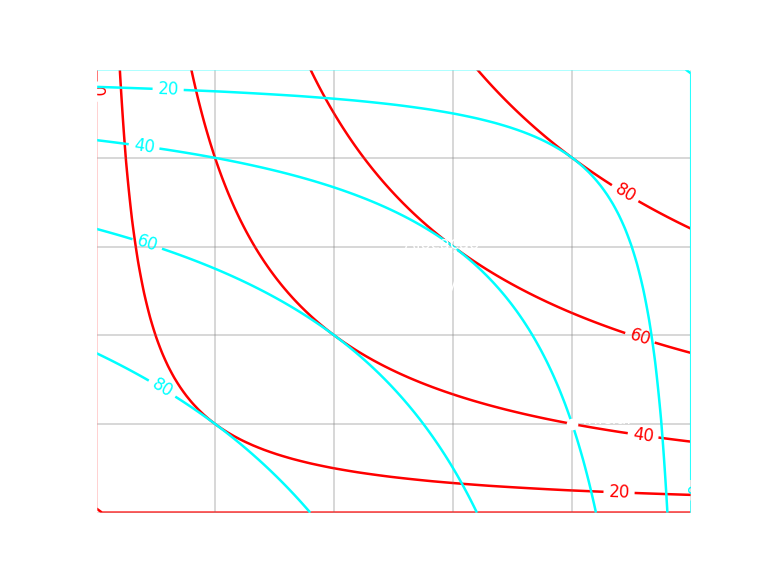
\includegraphics[scale=0.8]{cap32_1-caixa_edgeworth_1.png}
\end{figure}

Para analisar o gráfico da caixa, você deve se recordar das curvas de indiferença do consumidor. Uma mudança aqui é que estamos representando as preferências de dois consumidores ao mesmo tempo. As curvas vermelhas são do consumidor A e, consequentemente, as curvas azuis são do consumidor B.
\\
\\
Os eixos do consumidor B começam no canto superior-direita. Enquanto os eixos do consumidor A são os clássicos do plano cartesiano. Isso significa que cada ponto nesse gráfico possui 4 coordenadas associadas $(w_A^1, w_A^2, w_B^1, w_B^2)$ para a dotação e $(x_A^1, x_A^2, x_B^1, x_B^2)$ para a alocação final. A simetria que podemos ver nas quantidades se dá pela definição das alocações factíveis, onde para um ganhar, outro tem que ceder. 
\\
\\
Para ajudar no entendimento da leitura, eu coloquei umas setas indicando o sentido em que as quantidades crescem para cada consumidor.

\begin{figure}[H]
\centering
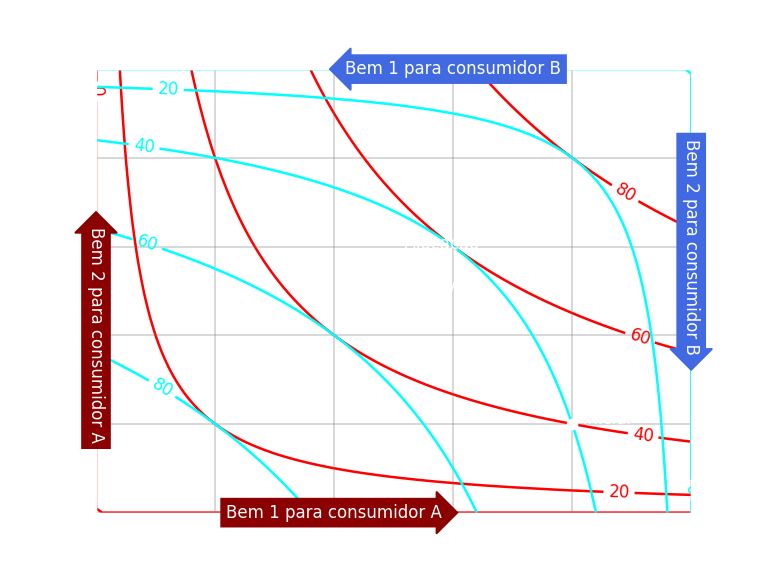
\includegraphics[scale=0.8]{cap32_1-caixa_edgeworth_2.png}
\end{figure}

Esse ferramental analítico nos permite mostrar todas as alocações factíveis, as preferências dos consumidores, a dotação inicial e a alocação final. Tudo isso de uma vez só. Não foi sem motivo que esse modelo foi adotado.

\section{As Trocas}

Nosso diagrama acima já deu um pequeno \textit{spoiler} sobre o que aconteceria se a dotação inicial fosse diferente da final. Para entender o processo de trocas, precisamos analisar o que se passa no momento em que os consumidores se encontram nas suas dotações iniciais.
\\
\\
No ponto da imagem, temos o encontro de duas curvas de indiferenças sendo uma para cada consumidor. O consumidor A gostaria de abrir mão do bem 1 para poder consumir mais do bem 2, já no caso de B, ele quer fazer o oposto, abrir mão de parte da quantidade do bem 2 para consumir mais do bem 1. Toda a área entre as curvas vermelha e azul representa uma região de melhoria mútua\footnote{Se você não entendeu esse argumento, tem que dar uma revisada urgente na teoria do consumidor. Melhor ir logo. Depois a gente continua essa aula.}.
\\
\\
O ponto onde os dois consumidores estão em melhor situação possível é o ponto de tangência das curvas de indiferença. As trocas ocorrerão até o ponto em que nenhuma melhoria seria possível sem a piora de um deles. No caso do exemplo, por acaso, o ponto final foi o da divisão igualitária, mas isso não é uma regra.\footnote{Explico melhor na próxima seção.}
\\
\\
As variações das quantidades em termo das dotações para o consumidor A são dadas por $|x_A^1 - w_A^1|$ para o bem 1 e $|x_A^2 - w_A^2|$ para o bem 2. Similarmente, $|x_B^1 - w_B^1|$ e $|x_B^2 - w_B^2|$, para o consumidor B.

\section{Alocações Eficientes no Sentido de Pareto}

Você já aprendeu no capítulo 01 sobre uma alocação eficiente no sentido de Pareto\footnote{Sem falar que toda hora esse conceito volta a ser usado ao longo do livro.}. Mas o professor resume aqui as principais caraterísticas dessa alocação. Então, vamos seguir o mesmo caminho.
\\
\\
Podemos descrever uma alocação eficiente de Pareto como tendo a seguintes propriedades:
\begin{itemize}
\item Não existe maneira de melhorar a situação de ninguém.
\item Não existe maneira de melhorar a situação de ninguém, sem que isso implique na piora de outra pessoa.
\item Todas as trocas que gerariam algum ganho foram feitas.
\item Não existe opção de troca que seja mutualmente vantajosa.
\end{itemize}

Essas características implicam que os pontos de eficiência sejam pontos em que as curvas de indiferença sejam tangentes entre si. Pois, se as curvas se cruzam, seria melhor para eles irem para algum ponto em uma curva mais alta, uma vez que, a região no interior do cruzamento de duas curvas é necessariamente, melhor para eles.
\\
\\
O conjunto de todos os pontos eficientes no sentido de Pareto, dentro de uma caixa de Edgeworth, é denominado de \textbf{conjunto de Pareto} ou \textbf{curva de contrato}. Como nossas funções de utilidade são iguais, a nossa curva de contrato é uma linha reta (se as preferências fossem outras, teríamos outro formato). Qualquer negociação de trocas que esteja num ponto desse subconjunto de alocações, será pareto-eficiente.

\begin{figure}[H]
\centering
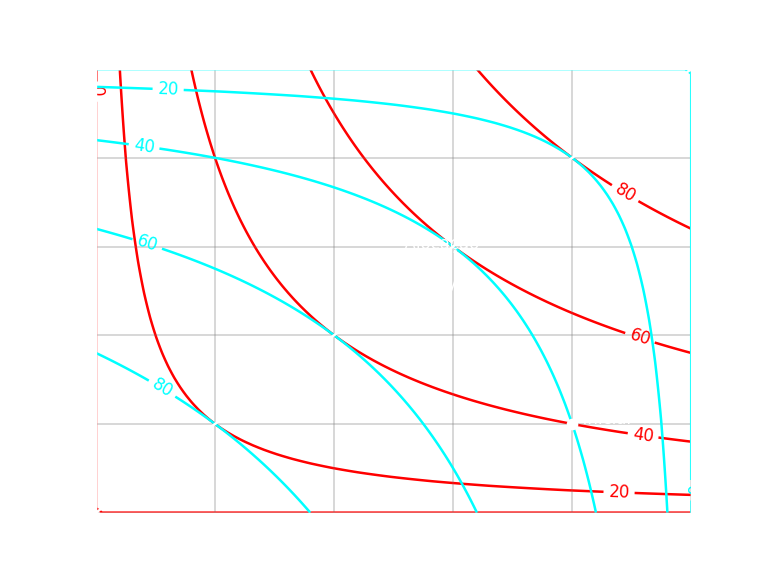
\includegraphics[scale=0.8]{cap32_3-caixa_edgeworth_1.png}
\end{figure}

\section{As Trocas de Mercado}

Até agora, sabemos que os agentes iniciam nas dotações inicias e terminam em algum ponto na linha de contrato. Como saber "onde"\ exatamente eles vão optar por parar de trocar? Para ter essa resposta, precisaremos adicionar mais informação sobre o comportamento dos nossos consumidores.
\\
\\
Adicionaremos a suposição que esse processo imitará o \textit{resultado} de um mercado competitivo\footnote{O resultado, não o processo.}.
\\
\\
Vamos colocar um terceiro indivíduo no processo. Ele agirá com um "leiloeiro"\ para A e B. O leiloeiro vai arbitrar um preço para A e B, e eles agirão a partir disso. Para cada preço arbitrado, os consumidores adaptarão as suas alocações finais aos preços de modo a maximizar suas utilidades. Nesse novo modelo, teremos  um novo dado, a dotação de preços $(p_1,p_2)$.
\\
\\
\textbf{Comentário:} Nós vimos no caso do duopólio e na teoria dos jogos que quando as interações ocorrem com poucos players, é provável que acabem sendo de maneira a não seguir a lógica da competição e sim da negociação. Mas o professor dá uma escapatória para o nosso modelo ao propor que interpretemos, ao invés de dois consumidores, dois grupos de consumidores que se comportam homogeneamente, podemos continuar nossa análise com esse ferramental. Ou então, podemos continuar pensando em duas pessoas, mas usando o modelo como uma representação do processo que ocorre para várias pessoas.
\\
\\
Vamos ver quais informações nós temos disponíveis para trabalhar agora: 1) Uma dotação inicial de bens; 2) Preços associados a cada bem; 3) Preferências de cada consumidor. Se você está com os conteúdos estudados na cabeça, sabe muito bem que tratamos essas variáveis no capítulo 5 (com a teoria da escolha) e no 9 (com as dotações).
\\
\\
Quando o leiloeiro determina o preço dos bens no mercado, ele automaticamente determina a renda de cada um dos participantes

$$renda_A = w_A^1 p_1 + w_A^2 p_2$$

Isso quer dizer que podemos, a partir da dotação inicial, descrever a restrição orçamentária via equação

$$ x_A^1 p_1 + x_A^2 p_2 = renda_A$$
$$ x_A^1 p_1 + x_A^2 p_2 = w_A^1 p_1 + w_A^2 p_2$$
$$ x_A^2 = [(w_A^1 p_1 + w_A^2 p_2) - x_A^1 p_1]/p2$$

Visualmente, a restrição orçamentária na caixa se apresenta igual ao problema do consumidor no início do livro, a diferença é que essa restrição se refere aos dois indivíduos.

\begin{figure}[H]
\centering
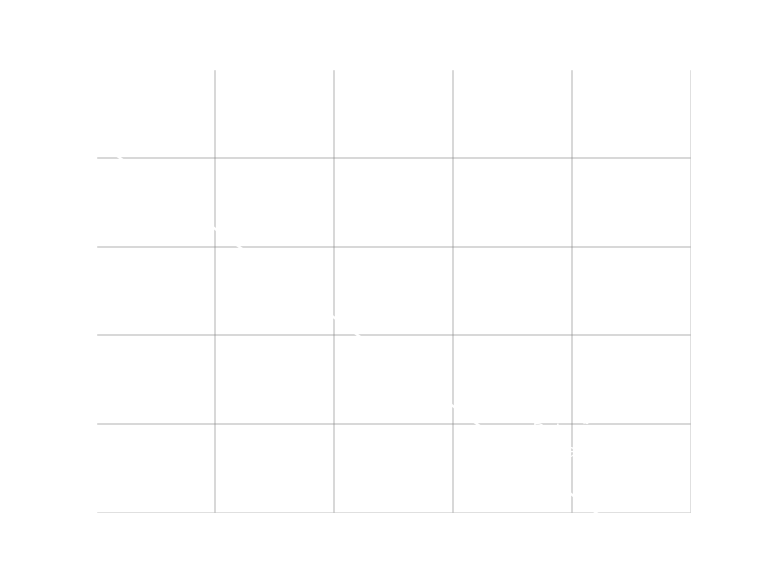
\includegraphics[scale=0.6]{cap32_4-caixa_edgeworth_1.png}
\end{figure}

Eu usei um ponto de dotação inicial diferente do que estamos trabalhando para mostrar um caso onde a alocação não é simétrica. Perceba que, se a alocação for desigual para algum consumidor, essa desigualdade será refletida na renda de cada consumidor. 
\\
\\
Agora vamos voltar para o nosso exemplo e acrescentar algumas curvas de indiferença para continuarmos nossa análise.

\begin{figure}[H]
\centering
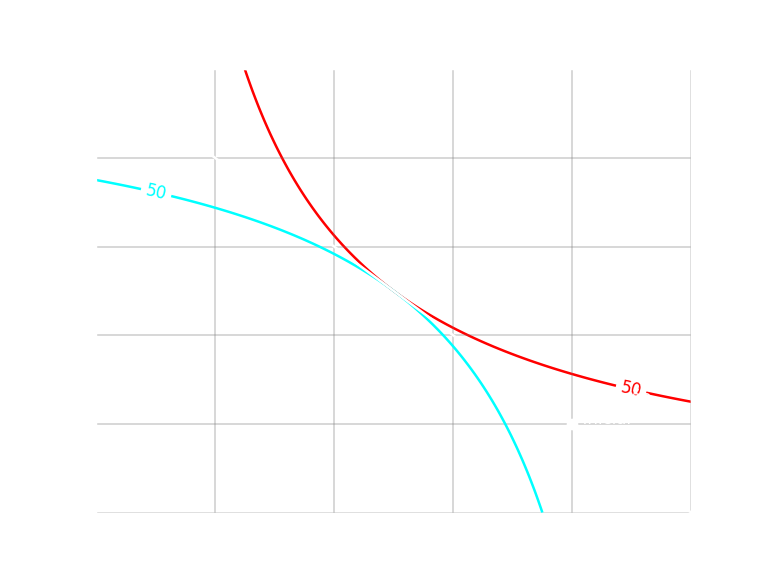
\includegraphics[scale=0.6]{cap32_4-caixa_edgeworth_2.png}
\end{figure}

Como vimos no capítulo 9. Os nossos consumidores aqui possuem incentivos de mudar suas alocações iniciais para maximizar suas utilidades. Você já sabe mas vamos recapitular alguns conceitos agora. A \textbf{demanda bruta} é o quanto o consumidor quer consumir de um bem dada sua renda (é obtida pelo cálculo da maximização com restrição lá do capítulo 5). Por sua vez, a \textbf{demanda líquida} ou \textbf{demanda excedente}, é dada pela equação $e_A^1 = x_A^1 - w_A^1$. Se $e_A1 < 0$, ele será um vendedor líquido, caso contrário, ele será um comprador. A partir de agora, usaremos o termo "demanda"\ para falar da \textbf{demanda bruta} e \textbf{demanda líquida ou excedente} caso queiramos falar desses outros conceitos.
\\
\\
Diferentemente do exemplo que estamos usando até agora (cujas utilidades possuem o mesmo formato), é possível que os preços arbitrados não produzam soluções. Ou seja, que as escolhas maximizadoras de cada consumidor não sejam compatíveis. Veja um caso onde modificamos os parâmetros da função de utilidade do consumidor A.

\begin{figure}[H]
\centering
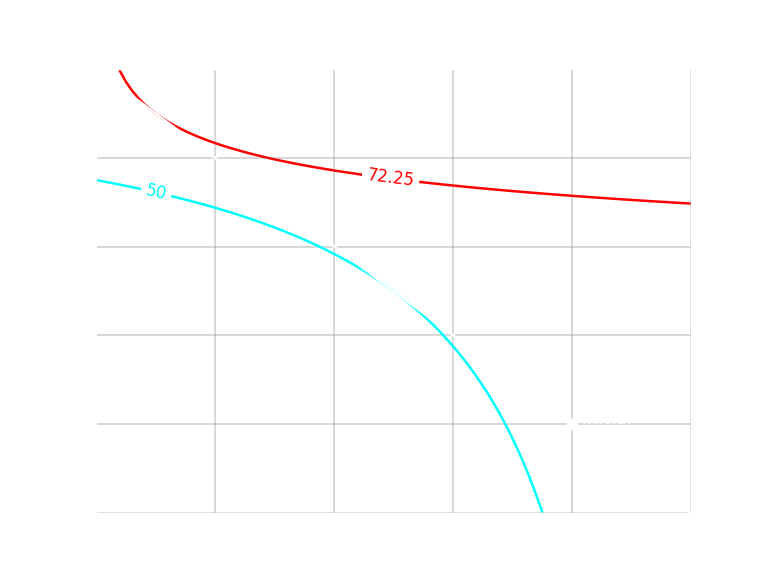
\includegraphics[scale=0.6]{cap32_4-caixa_edgeworth_3.png}
\end{figure}


Nessa situação, os agentes não conseguirão fazer as trocas porque, ao nível de preços dado, eles maximizam em pontos de alocação diferentes. Nós dizemos, nesse casos, que o mercado está em \textbf{desequilíbrio}.
\\
\\
Quando o mercado está em desequilíbrio o leiloeiro poderá intervir modificando os preços. Ele poderá aumentar o preço para os casos de excesso de demanda e reduzir em casos de excesso de oferta (a oferta aqui é quando a demanda líquida é negativa). 

\newpage

Você aprendeu lá no capítulo 2 o que acontece quando o preço de um bem se modifica em relação a outro. Isso mesmo, uma mudança na inclinação da restrição orçamentária. Vamos ver o que acontece quando o leiloeiro aumenta gradualmente o preço do bem 2 até um ponto onde as demandas sejam iguais. Você pode usar o zoom para enxergar melhor os gráficos.

\begin{figure}[H]
\centering
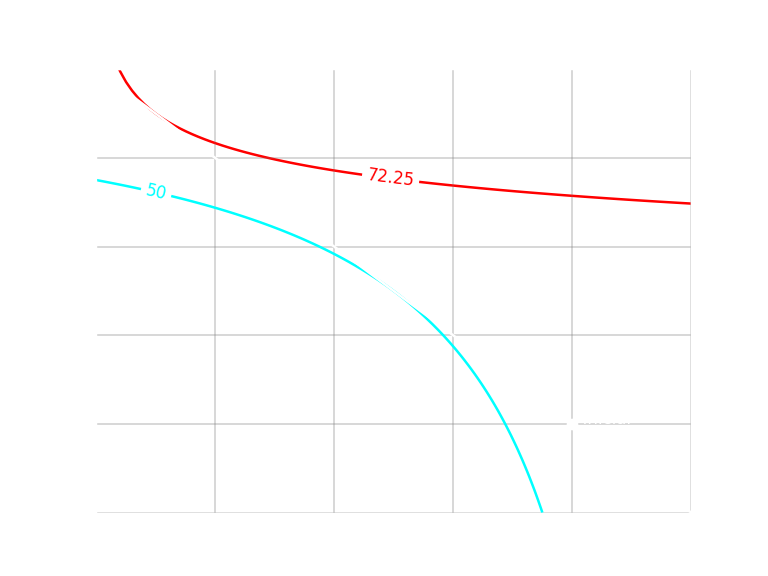
\includegraphics[scale=0.45]{cap32_4-caixa_edgeworth_4.png}
\end{figure}

\begin{figure}[H]
\centering
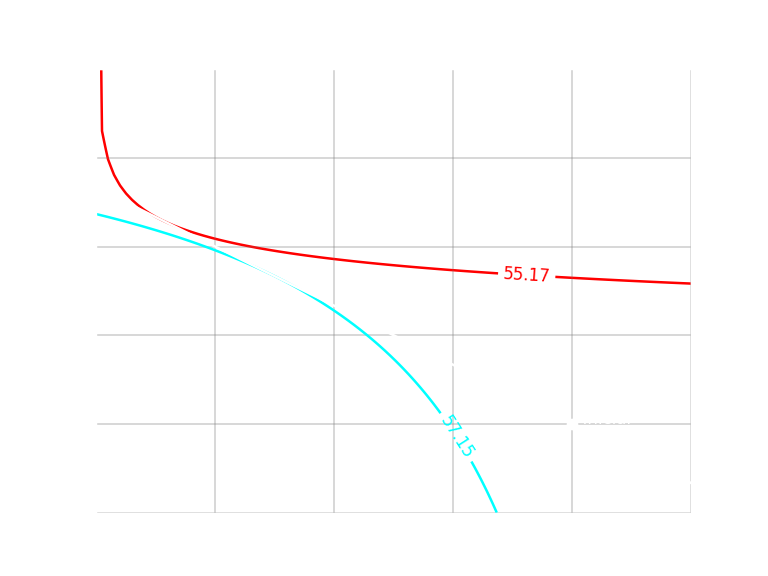
\includegraphics[scale=0.45]{cap32_4-caixa_edgeworth_5.png}
\end{figure}

\begin{figure}[H]
\centering
\includegraphics[scale=0.45]{cap32_4-caixa_edgeworth_6.png}
\end{figure}

\newpage

Nós vimos que, ao mudar os preços relativos dos bens, o leiloeiro conseguiu uma configuração da alocações onde as demandas são iguais. Nesse ponto, a quantidade total que cada pessoa deseja comprar é igual à quantidade ofertada no mercado. O mercado está em \textbf{equilíbrio}. Damos o nome desse tipo de solução em homenagem ao economista francês que primeiro estudou a teoria do equilíbrio geral, Leon Walras. Portanto, chamamos essa alocação de \textbf{equilíbrio walrasiano}\footnote{Outros nomes que esse arranjo recebe são \textbf{equilíbrio de mercado} e \textbf{equilíbrio competitivo}.}.
\\
\\
Nessa solução, todos os agentes escolhem a melhor cesta possível que podem pagar. Isso implica que a TMS entre os dois bens seja exatamente uma razão entre os preços. Contudo, como esses preços são iguais para todos os agentes, isso implica que todos deverão ter a mesma taxa marginal de substituição $-p_1/p_2$. Como as curvas de indiferença tangencia a restrição orçamentária na maximização, temos a demonstração do porquê as curvas de indiferença dos agentes serão tangentes entre si. 

\section{A Álgebra do Equilíbrio}

Agora que já entendemos como o processo de trocas pode levar a um equilíbrio competitivo, vamos construir a solução algébrica desse processo. Seja $x_A^1(p_1,p_2)$ a função demanda  bem 1 para o agente A e $x_B^1(p_1,p_2)$ a do função demanda do agente B. O equilíbrio walrasiano é obtido pelo par de preços $(p_1^*,p_2^*)$ de modo que

$$ x_A^1(p_1^*,p_2^*) + x_B^1(p_1^*,p_2^*) = w_A^1 + w_B^1 $$
$$ x_A^2(p_1^*,p_2^*) + x_B^2(p_1^*,p_2^*) = w_A^2 + w_B^2 $$

De modo que, no equilíbrio, temos uma igualdade entre a oferta e a demanda para os bens 1 e 2. Isso implica que a soma das demandas líquidas seja igual a zero. No equilíbrio (de duas pessoas), uma pessoa demanda exatamente o que a outra tem interesse em ofertar.
\\
\\
Podemos usar a nossa definição de demandas líquida $e(p_1,p_2) = [x(p_1^*,p_2^*) - w]$ na equação que estamos trabalhando para obtermos

$$ [x_A^1(p_1^*,p_2^*) - w_A^1] + [x_B^1(p_1^*,p_2^*) - w_B^1] = 0 $$
$$ [x_A^2(p_1^*,p_2^*) - w_A^2] + [x_B^2(p_1^*,p_2^*) - w_B^2] = 0 $$

Ou seja, as somas das demandas líquidas é igual a zero. Podemos reescrever nosso sistema como

$$ e_A^1(p_1*,p_2*) + e_B^1(p_1*,p_2*) = 0 $$
$$ e_A^2(p_1*,p_2*) + e_B^2(p_1*,p_2*) = 0 $$


Chamaremos de \textbf{função de demanda excedente agregada}, a soma das demandas líquidas dos indivíduos para cada par de preços. O equilíbrio é obtido pela existência de uma par de preços $(p_1,p_2)$ cuja demanda excedente agregada seja igual a zero para o bem 1 e para o bem 2.

$$z_1(p_1^*,p_2^*) = e_A^1(p_1*,p_2*) + e_B^1(p_1*,p_2*) = 0$$
$$z_2(p_1^*,p_2^*) = e_A^2(p_1*,p_2*) + e_B^2(p_1*,p_2*) = 0$$


O professor afirma que, se a demanda excedente agregada for igual a 0 para o bem 1. Ela sera, necessariamente, igual a 0 para o bem 2. Para provar essa afirmação nos vamos definir uma propriedade da função de demanda excedente agregada conhecida como \textbf{lei de Walras}.

\section{A Lei de Walras}

A lei de Walras afirma que

$$p_1 z_1(p_1,p_2) + p_2 z_2(p_1,p_2) \equiv 0$$

O interessante é que essa é uma \textit{identidade}. Isso quer dizer que temos essa relação para qualquer par de preços, mesmo os que não produzam um equilíbrio. A demonstração decorre do fato que as demandas estão sujeitas as restrições orçamentárias

$$p_1x_A^1(p_1,p_2) + p_2x_A^2(p_1,p_2) \equiv p_1w_A^1 + p_2w_A^2$$
$$p_1x_B^1(p_1,p_2) + p_2x_B^2(p_1,p_2) \equiv p_1w_B^1 + p_2w_B^2$$

Trazendo as dotações para o lado esquerdo da equação

$$p_1[x_A^1(p_1,p_2) - w_A^1] + p_2[x_A^2(p_1,p_2) - w_A^2] \equiv 0$$
$$p_1[x_B^1(p_1,p_2) - w_B^1] + p_2[x_B^2(p_1,p_2) - w_B^2] \equiv 0$$

Reescrevendo usando a notação da demanda excedente

$$p_1[e_A^1(p_1,p_2)] + p_2[e_A^2(p_1,p_2)] \equiv 0$$
$$p_1[e_B^1(p_1,p_2)] + p_2[e_B^2(p_1,p_2)] \equiv 0$$

Essas equações nos dizem que o \textit{valor} (ou seja, preço vezes quantidade do bem 1 + preço vezes quantidade do bem 2) da demanda líquida de cada agente é igual a zero. Se somarmos as duas identidades, chegaremos a

$$p_1[e_A^1(p_1,p_2)] + p_2[e_A^2(p_1,p_2)] + 
p_1[e_B^1(p_1,p_2)] + p_2[e_B^2(p_1,p_2)] \equiv 0$$
$$p_1[e_A^1(p_1,p_2) + e_B^1(p_1,p_2)] + p_2[e_A^2(p_1,p_2) + e_B^2(p_1,p_2)] \equiv 0$$

Veja que os termos dentro dos colchetes são exatamente as funções de demanda excedente agregadas. Ou seja

$$p_1[z_1(p_1,p_2)] + p_2[z_2(p_1,p_2) ] \equiv 0$$

Chegamos exatamente na lei de Walras. Que é o que queríamos mostrar. Como o valor das demandas líquidas de cada agente é igual a zero. O motivo disso é que a soma das demandas líquidas também será igual a zero.\footnote{Eu demorei um tempo até entender essa frase. Só segue a diante se realmente tu entender.}
\\
\\
Como a lei de Walras se aplica para \textit{qualquer} nível de preços, ela também é válida para o caso particular onde a demanda a função de demanda excedente agregada para o bem 1 seja igual a zero:

$$z_1(p_1^*,p_2^*) = 0$$

A lei de Walras, que acabamos de ver, nos afirma que

$$p_1 z_1(p_1,p_2) + p_2 z_2(p_1,p_2) = 0$$

Juntando as duas coisas, temos que

$$ p_2 z_2(p_1,p_2) = 0$$

Para qualquer $p_2 \geq 0$, será obrigatório que

$$z_2(p_1,p_2) = 0$$

Isso nos dá a certeza que, ao encontramos um par de preços de equilíbrio para o bem 1 cuja a demanda líquida agregada seja igual a zero. A demanda líquida agregada do bem 2 também será igual a zero.
\\
\\
Esse mesmo raciocínio pode ser generalizado para o equilíbrio em $k$ bens. Nesse caso, nós precisaremos encontrar a lista de preços $(p_1,p_2,...,p_{k-1},p_k)$ que produza o equilíbrio em $k - 1$ mercados. A lei de Walras nos assegura que o mercado do bem $k$ também estará automaticamente em equilíbrio.

\section{Preços Relativos}

Alguns de vocês podem estar um pouco céticos com a afirmação do último parágrafo. Como podemos encontrar $k$ preços de equilíbrio olhando apenas para $k - 1$ mercados? A verdade é que só existem $k - 1$ preços independentes. 
\\
\\
Como as relações no modelo de trocas se dão pela equivalência entre as dotações iniciais e as preferências, o que importa entre os preços não é seu valor nominal e sim seu valor relativo. No exemplo de como o leiloeiro aumentou o preço do bem 2 afim de chegar no equilíbrio do mercado, nós saímos da relação de preço $p_1 = p_2 = 1$ para uma relação $2p_1 = p_2$ (ou seja, $p_2$ é o dobro de $p_1$). Entretanto, nós chegaríamos no mesmo equilíbrio se o leiloeiro \textit{reduzisse} preço do bem 1 para 0,5.
\\
\\
Isso nos permite escolher um dos preços como um \textbf{numerário}. Bastando multiplicar todos os $k$ preços por $1/p_k$, chegaremos a um sistema com $k - 1$ preços (que agora estarão dividos por $p_k$) e $k - 1$ equações. O sistema vai ficar algo como

$$\frac{p_1}{p_k}x_1(p_1,p_2,...,p_{k-1}) \ + $$
$$\frac{p_2}{p_k}x_2(p_1,p_2,...,p_{k-1}) \ + $$ 
$$ \vdots $$
$$\frac{p_{k-1}}{p_k}x_{k - 1}(p_1,p_2,...,p_{k-1}) \ + $$
$$x_{k}(p_1,p_2,...,p_{k-1}) = 0$$

Atenção aqui: Isso quer dizer que o modelo de equilíbrio que estamos trabalhando só pode determinar o equilíbrio das quantidades através de \textbf{preços relativos}. O que não é uma restrição que faça grande diferença na realidade.

\subsection{Um Exemplo algébrico do equilíbrio}

Vamos colocar toda essa álgebra em ação usando as funções de utilidade do tipo Cobb-Douglas. Seja $u_a(x_1,x_2) = (x_A^1)^{a_A}(x_A^2)^{b_A}$ sendo $a_A + b_A = 1$, a função de utilidade do consumidor A e semelhantemente para B. O sistema de equações de demandas para cada agente em cada mercado será dado por

$$ x_A^1(p_1,p_2,m_A) = a_A \frac{m_A}{p_1} $$
$$ x_A^2(p_1,p_2,m_A) = b_A \frac{m_A}{p_2} $$
$$ x_B^1(p_1,p_2,m_B) = a_B \frac{m_B}{p_1} $$
$$ x_B^2(p_1,p_2,m_B) = b_B \frac{m_B}{p_2} $$

Os parâmetros a e b são os expoentes das funções de utilidade. O sobrescrito em cada um deles indica a qual agente eles se referem.
\\
\\
As rendas $m$ são dadas pelos preços multiplicados pela quantidade na dotação inicial de cada agente:

$$m_A = p_1w_A^1 + p_2w_A^2$$
$$m_B = p_1w_B^1 + p_2w_B^2$$

substituindo no sistema de equações anterior teremos que

$$ x_A^1(p_1,p_2) = a_A \frac{p_1w_A^1 + p_2w_A^2}{p_1} $$
$$ x_A^2(p_1,p_2) = b_A \frac{p_1w_A^1 + p_2w_A^2}{p_2} $$
$$ x_B^1(p_1,p_2) = a_B \frac{p_1w_B^1 + p_2w_B^2}{p_1} $$
$$ x_B^2(p_1,p_2) = b_B \frac{p_1w_B^1 + p_2w_B^2}{p_2} $$


As demandas excedentes agregadas são dadas pelas somas das demandas excedentes (que nada mais são do que as demandas menos as dotações). No nosso caso, são iguais a

$$z_1(p_1,p_2) = 
a_A \frac{p_1w_A^1 + p_2w_A^2}{p_1} + 
a_B \frac{p_1w_B^1 + p_2w_B^2}{p_1} - w_A^1 - w_B^1$$

$$z_2(p_1,p_2) = 
b_A \frac{p_1w_A^1 + p_2w_A^2}{p_2} + 
b_B \frac{p_1w_B^1 + p_2w_B^2}{p_2} - w_A^2 - w_B^2$$

Essas equações satisfazem a lei de Walras. Se você duvidar disso, o que é um ótimo sinal, pode aplicar exatamente o mesmo processo feito na seção 32.6.
\\
\\
Ao escolhermos $p_2$ como nosso numerário, podemos dividir os preços por $p_2$ de modo que $p_2/p_2 = 1$. Para simplificação, vamos adotar a notação $p_1 = p_1/p_2$. Acabaremos com um sistema igual a

$$z_1(p_1,1) = 
a_A \frac{p_1w_A^1 + w_A^2}{p_1} + 
a_B \frac{p_1w_B^1 + w_B^2}{p_1} - w_A^1 - w_B^1$$

$$z_2(p_1,1) = 
b_A (p_1w_A^1 + w_A^2) + 
b_B (p_1w_B^1 + w_B^2) - w_A^2 - w_B^2$$

No equilíbrio, nós vimos que as demandas excedentes agregadas são iguais a zero, então, vamos pegar uma dessas duas equações e resolver $p_1$ para o caso igual a zero. Se você fizer isso para a primeira, chegará num resultado igual a

$$p_1^* = \frac{a_A w_A^2 + b_A w_B^2}{a_B w_A^1 + b_B w_B^1}$$

Esse valor de $p_1$ é o valor cuja demanda excedente agregada para o bem 1 é igual a zero. Pela lei de Walras que acabamos de ver, já sabemos então que a demanda excedente do bem 2 também será igual a zero.

\section{A Existência de Equilíbrio}

Como esse curso é nível graduação, não entraremos muito fundo nos aspectos formais de alguns tópicos. Nos níveis de pós-graduação, os ferramentais matemáticos formais são a principal maneira de demonstrar conceitos e derivar conclusões. Umas dessas conclusões que estudaremos brevemente diz respeito à \textbf{existência de um equilíbrio competitivo}, ou seja, investigaremos como podemos afirmar que sempre existe \textit{pelo menos algum} conjunto de preços que iguale oferta e demanda nos mercados.
\\
\\
\textbf{Comentário:} Para aqueles com mais curiosidade. Eu recomendo uma consulta no capítulo 15 do Mas-Colell (1995), capítulo 21 do Varian: Microeconomic Analysis (1992), capítulo 05 do Kreps (1990) e capítulo 05 do Jehle (2011). Mas fica aqui o aviso, o ferramental matemático é bem mais avançado do que estamos trabalhando nesse curso.
\\
\\
Como o próprio professor Kreps expõe no livro dele a resposta para a pergunta "Sempre existe um equilíbrio walrasiano para uma economia de trocas qualquer"\ geralmente será não. Então o que os cientistas trabalharam para responder foi uma versão um pouco diferente dessa pergunta: "Sob quais condições, é garantido que exista algum equilíbrio em uma economia de trocas?". A resposta (versão graduação) para essa pergunta é que a função de demanda excedente deve ser uma \textbf{função contínua}.
\\
\\
A continuidade é uma característica das funções e possui um punhado de definições existentes. O professor Varian coloca uma versão bem resumida que vamos usar (mas eu também foi colocar uma um pouco mais formal como comentário opcional). Uma função é chamada de contínua se \textit{pequenas variações} na suas variáveis independentes resultam em \textit{pequenas variações} variáveis dependentes. Ou seja, não temos \textit{grandes saltos} ou \textit{quebras} no gráfico dessas funções.
\\
\\
\textbf{Comentário Opcional:} Uma definição mais formal de função contínua (a definição de Cauchy) pode ser achada na página 534 do livro "Advanced Microeconomics"\ do professor Jehle. Seja $D$ um subconjunto de $\mathbb{R}^m$ e seja $f : D \shortrightarrow \mathbb{R}^n$. Então, a função f será contínua se, no ponto, $\mathbf{x} \in D$ se, para todos os $\epsilon > 0$, existir um $\delta >0$ de modo que $f(B_{\delta}(\mathbf{x}^0 \cap D) \subset B_{\epsilon}(f(\mathbf{x}^0)$.\footnote{Isso aqui é para vocês terem um gostinho de como é o conteúdo nos níveis mais avançados.}
\\
\\
Mas agora precisamos saber quais são as condições para que a função de demanda excedente seja contínua. Temos dois tipos de condições. A primeira é que as funções de demanda individuais sejam contínuas (que por sua vez tem como condição que as preferências dos consumidores sejam convexas). A segunda é que, mesmo que algumas pessoas tenham comportamento descontínuo, se essas forem pequenas em relação ao total do mercado, a função de demanda ainda pode ser contínua (que é um pressuposto bem razoável em se tratando de um mercado competitivo).

\section{Equilíbrio e Eficiência}

A questão a eficiência diz respeito a comprovação de que um equilíbrio de mercado é um modelo eficiente de Pareto. A comprovação é simples: Como os pontos da curva de contrato são os pontos onde as curvas de utilidade mais altas, ou seja, com maior valor, tangenciam a curva de dotação dos agentes, não há possibilidade de algum deles obter qualquer melhoria preferida pois a escolha de maior utilidade já foi satisfeita dada a restrição orçamentária.

\section{A Álgebra da Eficiência}

Podemos demonstrar o argumento da seção anterior de maneira algébrica. Para isso vamos partir da hipótese de que o equilíbrio de mercado \textbf{não} é eficiente no sentido de Pareto.
\\
\\
\textbf{Comentário:} Essa seção é uma boa demonstração de como funciona uma demonstração formal. Nós queremos provar uma hipótese mas a abordagem que o professor optou foi partir da negação dessa hipótese. Pode parecer estranho, mas a ideia é simples: se partimos da ideia que a nossa hipótese é falsa, somos capazes de chegar a um resultado válido? Se a resposta for não, isso significa que nossa hipótese só pode ser verdadeira.\footnote{O nome dessa técnica de demonstração é "prova por contradição".}
\\
\\
Dizer que o equilíbrio de mercado não é eficiente no sentido de Pareto implica na existência de uma alocação possível $(y_A^1,y_A^2,y_B^1,y_B^2)$ de modo que

\newpage

$$y_A^1 + y_B^1 = w_A^1 + w_ B^1$$
$$y_A^2 + y_B^2 = w_A^2 + w_ B^2$$

onde, se essa alocação y for preferida à outra alocação x será verdade que

$$(y_A^1 + yA2) \succ_A (x_A^1 + x_A^2)$$
$$(y_B^1 + yB2) \succ_B (x_B^1 + x_B^2)$$

Os símbolos "$\succ_A$" e "$\succ_B$" significam as preferências de A e B.
\\
\\
As primeiras equações nos dizem que a alocação y é factível. As segundas relações nos dizem que os agentes A e B preferem a alocação y em detrimento da alocação x.
\\
\\
Mas veja que, pelo conceito de equilíbrio de mercado, os agentes estão nas alocações que maximizam a sua utilidade dada sua restrição orçamentária. Isso implica em dizer que, se y é preferido ao equilíbrio, essa alocação precisa ser, obrigatoriamente, mais cara que a alocação do equilíbrio, ou seja, está acima da restrição orçamentária de cada agente. Esse argumento pode ser traduzido na forma algébrica

$$p_1y_A^1 + p_2y_A^2 > p_1w_A^1 + p_2w_A^2$$
$$p_1y_B^1 + p_2y_B^2 > p_1w_B^1 + p_2w_B^2$$

Somando as duas inequações, teremos

$$p_1(y_A^1 + y_B^1) + p_2(y_A^2 + y_B^2) > p_1(w_A^1 + w_ B^1) + p_2(w_A^2 + w_ B^2)$$

Mas se voltarmos nas duas primeiras equações e substituirmos o lado esquerda dessa inequação, chegaremos ao resultado

$$p_1(w_A^1 + w_ B^1) + p_2(w_A^2 + w_ B^2) > p_1(w_A^1 + w_ B^1) + p_2(w_A^2 + w_ B^2)$$

O que é uma contradição, mas isso é exatamente o resultado que queríamos chegar.
\\
\\
Como derivamos uma contradição partindo da negativa da nossa hipótese, podemos concluir que a hipótese original é verdadeira. Desse modo, podemos afirmar que os equilíbrios de mercado são eficientes no sentido de Pareto.
\\
\\
Essa conclusão é tão importante que a comunidade científica denominou como \textbf{Primeiro Teorema da Teoria Econômica do Bem-Estar}.
\\
\\
Esse teorema afirma que as alocações obtidas em um mercado competitivo serão eficientes no sentido de Pareto. Atente para o fato que o teorema não afirma nada sobre outras características como, por exemplo, a distribuição da renda. A prova disso é que a alocação 100\% para o agente A e 0\% pra o B é eficiente no sentido de Pareto. O resultado pode até não ser socialmente aceitável ou desejável, mas será necessariamente eficiente.
\\
\\
\textbf{Comentário:} Aqui nós temos um exemplo onde revisitamos o monopólio só que dessa vez dentro de uma caixa de Edgeworth. Vemos como um monopólio acaba alocando de maneira ineficiente os recursos para poder maximizar seu retorno. Ao invés de escolher o preço onde a curva de indiferença dos dois agentes tangencia a restrição orçamentária, o monopolista escolhe o ponto onde a curva de indiferença dele tangencia a curva de preço-consumo do outro agente. Também percebemos que um monopolista perfeitamente discriminador é capaz de criar uma alocação eficiente no sentido de Pareto.

\section{Eficiência e Equilíbrio}

O primeiro teorema de bem-estar nos diz que todo equilíbrio de mercado é eficiente no sentido de Pareto. Mas será possível afirmar que toda alocação eficiente no sentido de Pareto pode ser alcançada por um conjunto de preços definidos por um mercado competitivo? A resposta é sim, mas depende de algumas condições.
\\
\\
Devemos lembrar que um equilíbrio de mercado é o ponto onde as curvas de indiferença dos agentes tangencia a restrição orçamentária em \textbf{um único ponto}. O problema é que um equilíbrio de Pareto não tem nenhuma relação com a restrição orçamentária. Então, sempre que as curvas de indiferença são tangentes, temos um equilíbrio de Pareto.
\\
\\
A nossa condição reside justamente na relação entre esses dois conceitos. Se as preferências dos agentes são \textbf{convexas}, para cada equilíbrio de Pareto, haverá alguma lista de preços que possa determinar aquela alocação. Essa condição (de convexidade) das preferências recebeu o nome de \textbf{Segundo Teorema do Bem-Estar}.
\\
\\
A demonstração que o professor nos dá é gráfica e pode ser observada no material original.

\section{Implicações do 1º Teorema do Bem-Estar}

Esses teoremas que vimos são de grande relevância para a teoria econômica. Mesmo que nosso estudo ainda seja em nível básico, saiba que essas demonstrações podem ser expandidas para um número arbitrário de agentes e bens. Essas conclusões são fundamentais para a elaboração de modelos de alocação de recursos.
\\
\\
Existem alguns pressupostos que fazem parte do teorema que merecem ser explicitados para melhor compreensão:

\begin{itemize}
\item Os agentes só se preocupam com seu consumo de bens e não com a escolha dos demais agentes. Quando existe essa relação entre os agentes, dizemos que há uma \textbf{externalidade no consumo} que pode levar a um resultado ineficiente de Pareto.

\item Os agentes agem de maneira competitiva. Nós já vimos que o modelo de dois consumidores é apenas uma ferramenta didática.

\item O teorema só é relevante em um contexto de equilíbrio competitivo. Se temos poder de mercado (que ocorre quando temos poucos agentes) esse teorema não se aplicaria.
\end{itemize}

Esses pressupostos constituem um estrutura poderosa (e também uma delimitação clara) para a utilização do modelo competitivo de alocação. Sempre que tivermos relativa confiança que determinado mercado é competitivo, os consumidores só precisarão saber os preços para alocar suas dotações de maneira eficiente. Essa redução da necessidade de informação para a tomada da decisão de consumo é um forte argumento para adoção desse modelo quando precisamos alocar recursos escassos.

\section{Implicações do 2º Teorema do Bem-Estar}

O segundo teorema afirma que, se as preferências são convexas, podemos alcançar qualquer alocação eficiente de Pareto pelo sistema de preços.
\\
\\
A implicação poderosa desse teorema é que as discussões de eficiência e distrição da riqueza podem ser separadas. Os preços alocam a renda via mecanismo de escassez relativa. Já a distribuição diz respeito a quantidade que os agentes poderão comprar.
\\
\\
Uma vez que os agentes maximizam suas escolhas ao nível de preços dados e às suas restrições orçamentárias. Em um determinado contexto é muito desigual na dotação inicial, poderíamos redistribuir parte da dotação de um agente para o outro. O que o segundo teorema nos afirma é que o equilíbrio alcançado a partir dessa nova dotação é eficiente no sentido de Pareto.
\\
\\
Perceba então que, se a sociedade tem como meta a redução de desigualdade entre as pessoas, uma mudança na \textbf{dotação} (e consequentemente na renda) via transferência entre os agentes produziria uma alocação eficiente de Pareto. Do ponto  de vista teórico, a realocação das dotações não produzirá distorções no mercado.
\\
\\
Não é incomum que, em busca de reduzir a desigualdade, as discussões de política econômica defendam uma intervenção nas decisões de preços. Enquanto os impostos baseados na dotação de bens dos consumidores não geram ineficiência, os impostos que dependem das escolhas dos consumidores (baseados no consumo) geram ineficiência.
\\
\\
\textbf{Comentário:} A aplicação da teoria não faz parte do escopo desse curso mas vale a pena começar a procurar materiais de economia aplicada para você perceber como esses mecanismos discutidos são usados como ferramentas analíticas. Eu tentei resumir essa parte mais teórica, mas você deve ler o material original.

\section{Apêndice Matemático do equilíbrio}

Aqui veremos como o problema da determinação do equilíbrio é resolvido com uso do cálculo. Dada a utilidade qualquer do agente B fixa $\overline{u}$, o problema da maximização da utilidade total do mercado pode ser formalizado como

\begin{center}
\LARGE $\stackrel{máx}{\text{\small $x_A^1,x_A^2,x_B^1,x_ B^2$}} \ \ \stackrel{u_A(x_A^1,x_A^2)}{\ }$ \\
\ 
\\
\normalsize de modo que $u_B(x_B^1,x_B^2) = \overline{u}$ \\
$x_A^1 + x_B^1 = w^1$ \\
$x_A^2 + x_B^2 = w^2$
\end{center}

Você aprendeu no capítulo 05 como fazer uma maximização de uma função objeto dada uma restrição. A novidade aqui é que temos 3 condições de restrições. Pode até assustar numa primeira vista, mas não é nada impossível.
\\
\\
Primeiramente, podemos escrever nosso problema em forma de uma Lagrangiana 

$$L(x_A^1,x_A^2,x_B^1,x_B^2) = u_A(x_A^1,x_A^2) - \lambda(u_B(x_B^1,x_B^2) - \overline{u}) $$ 
$$ - \mu_1(x_A^1 + x_B^1 - w^1) - \mu_2(x_A^2 + x_B^2 - w^2)$$

Onde o $\lambda$ é o nosso conhecido multiplicador Lagrangiano, só que aqui, aplicada para a utilidade de B e $\mu$ são os multiplicadores de Lagrange nas restrições dos recursos.
\\
\\
As condições de primeira ordem para maximização da nossa Lagrangiana a respeito das 4 variáveis são:

$$\frac{\partial L}{\partial x_A^1} = \frac{\partial u_A}{\partial x_A^1} - \mu_1 = 0$$
$$\frac{\partial L}{\partial x_A^2} = \frac{\partial u_A}{\partial x_A^2} - \mu_2 = 0 $$
$$\frac{\partial L}{\partial x_B^1} = -\lambda \frac{\partial u_B}{\partial x_B^1} - \mu_1 = 0 $$
$$\frac{\partial L}{\partial x_B^2} = -\lambda \frac{\partial u_B}{\partial x_B^2} - \mu_2 = 0 $$

Eu não sei você, mas quando eu olhei essa passagem, eu fiquei com dúvida porque lá no capítulo 05 ele deriva a Lagrangiana em relação ao lambda também. A questão é que nós não precisamos fazer isso obrigatoriamente. Se não nos atrapalhar que as soluções de maximização sejam funções dos multiplicadores de Lagrange, podemos manter as condições de primeira ordem apenas para as variáveis que queremos.\footnote{Eu queria explicar melhor, mas eu preciso que você tenha feito o dever de casa se está nessa parte do curso. Não dá pra ter dúvidas sobre isso nessa altura do campeonato.}
\\
\\
Lá no capítulo sobre as preferências, nós aprendemos que a taxa marginal de substituição é obtida quando, dada uma função de utilidade $u(x_1,x_2)$, a derivada parcial de $u$ em função de $x_{1}$ divida pela derivada parcial de $u$ em relação à $x_{2}$. Ou seja

$$TMS_{A} = \frac{\partial u_A / \partial x_{A}^1 }{\partial u_A / \partial x_{A}^2} = \frac{\mu_{1} }{ \mu_{2} }$$

Que é o que obtemos quando dividimos a primeira equação pela segunda.
\\
\\
Se fizermos a mesma coisa para as equações 3 e 4, teremos

$$TMS_{B} = \frac{\partial u_A / \partial x_{B}^1 }{\partial u_A / \partial x_{B}^2} = \frac{\mu_{1} }{ \mu_{2} }$$

A explicação desse igualdade já é conhecida: no equilíbrio, as taxas marginais de substituição são iguais para os dois mercados.
\\
\\
Também sabemos que, no equilíbrio de um mercado competitivo, as TMS são iguais aos preços, ou seja

$$	\frac{\partial u_A / \partial x_{A}^1 }{\partial u_A / \partial x_{A}^2} = \frac{\partial u_A / \partial x_{B}^1 }{\partial u_A / \partial x_{B}^2} = \frac{ p_{1} }{ p_{2} } $$

Observe que temos uma equivalência entre os multiplicadores de Lagrange $\mu$ e os preços. Eles até têm nomes especiais, nesse contexto, podem ser chamamos de \textbf{preços-sombra} ou \textbf{preços de eficiência}.
\\
\\
Esse igualdade decorre do fato que toda alocação eficiente de Pareto deve satisfazer as igualdades das TMS em relação aos multiplicadores de Lagrange. E, por outro lado, todo equilíbrio em mercado competitivo, deve igualar a taxa marginal de substituição pela divisão dos preços.

%%%%%%%%%%%%%%%%%%%%%%%% CHAPTER %%%%%%%%%%%%%%%%%%%%%%%%
\chapter{Produção}

Você deve ter sentido falta do componente da produção no nosso modelo de equilíbrio geral. Tal qual o capítulo anterior, nós vamos nos valer de simplificações para poder avançarmos na construção do modelo. Aqui, vamos supor apenas um único consumidor, uma única empresa e dois bens. O nome dado a esse tipo de modelo foi \textbf{economia de Robinson Crusoé}\footnote{Caso você não conheça, Robinson Crusoé é um personagem de um romance que vive sozinho em uma ilha.}.Como anteriormente, os resultados obtidos aqui podem ser generalizados para um número arbitrário de agentes.

\section{A Economia de Robinson Crusoé}

Na nossa hipótese fantasiosa, Robinson Crusoé terá um duplo papel: ele produzirá todo o montante de alimento (cocos) e será o único consumidor. Desse modo, ele pode escolher, para cada período de tempo, entre gastar energia coletando cocos ou descansar na praia.
\\
\\
Diferentemente da nossa caixa de Edgeworth, aqui teremos a volta da \textbf{função de produção}. Suporemos que a função de produção de cocos tenha rendimentos marginais decrescentes ao longo do tempo trabalhado. No gráfico abaixo podemos ver algumas curvas de indiferença e a função de produção.

\begin{figure}[H]
	\centering
	\includegraphics[scale=0.6]{cap33_1-economia_robinson.png}
\end{figure}

O ponto de maximização ocorre na tangência entre a função de produção e a curva de indiferença mais alta.

\section{Crusoé S.A.}

Essa é a seção mais estranha que eu já vi em um livro didático. Vá ler o material original. Mas a ideia, por mais estranha que seja, faz todo sentido. Ao colocarmos uma empresa maximizadora de lucros dentro do nosso modelo, novas variáveis surgem como, por exemplo, salário, lucro e preço. O objetivo é construir um modelo de equilíbrio geral que seja capaz de igualar, simultaneamente, os preços no mercado de bens e no mercado de trabalho.
\\
\\
A estratégia usada para simplificar o processo foi tornar o produto - que no nosso caso é coco - como um numerário. Isso simplifica a análise porque agora só temos que definir o salário e o lucro em termos do nosso numerário.

\section{A Empresa}

O problema de empresa é simples de entender. O objetivo do empresário é maximizar o seu lucro $\pi$. Para isso, ele terá que decidir a quantidade produzida no mercado $C$. Como estamos usando o coco como numerário, a receita da empresa será dada pela quantidade total produzida e vendida no mercado. Para poder produzir, a empresa terá que contratar uma quantidade $L$ de trabalho, que será pago por um salário $w$.
\\
\\
Podemos traduzir esse raciocínio acima na seguinte equação:

$$ \pi = C - wL $$

Ou, se estivermos interessados na quantidade de produção, podemos reescrever como:

$$ C = \pi + wL $$

Não é difícil ver que essa função função de primeiro grau é uma curva de \textbf{isolucro} lá do capítulo 20. Desse modo, podemos ver, a partir de uma nível inicial de lucro $\pi^*$, a quantidade de cocos que manteria o lucro constante após o pagamento da mão de obra.
\\
\\
A maximização nesse caso, ocorre no ponto onde a reta de isolucro intercepta a curva da função de produção. Esse é o ponto onde a empresa consegue o maior retorno possível. O gráfico abaixo ilustra bem essa situação

\begin{figure}[H]
	\centering
	\includegraphics[scale=0.6]{cap33_3-max_lucro.png}
\end{figure}

Com isso, conseguimos determinar que, dado o salário $w$ e a função de produção, a empresa contratará a quantidade de trabalho que permita o lucro máximo. Como no nosso exemplo o único acionista é o Robinson, ele poderá usufruir do consumo de $\pi^*$ cocos oriundos do seu lucro como empresário.

\section{O Problema de Robinson}

Após receber seus dividendos, Robinson tem que escolher entre usufruir dos cocos e descansar ou trabalhar na coleta de mais cocos (recebendo seu devido salário). Nós já vimos no capítulo 9 o problema de maximização da utilidade com trabalho. Esse problema é uma adaptação daquele. Robinson escolherá ofertar a quantidade de trabalho que produza a maior utilidade possível dada sua restrição orçamentária

\begin{figure}[H]
	\centering
	\includegraphics[scale=0.6]{cap33_4-max_trabalho.png}
\end{figure}

Com esse ponto, conseguimos determinar a oferta de trabalho pela igualdade entre a TMS do consumo pelo lazer e o salário. Exatamente o que vimos no capítulo 9.

\section{Colocando os dois Juntos}

Agora que sabemos como Robinson se comportará tanto como acionista da Crosué S.A. como trabalhador. Podemos colocar esses dois equilíbrios num mesmo gráfico para ver como as variáveis se comportam juntas.

\begin{figure}[H]
	\centering
	\includegraphics[scale=0.5]{cap33_5-equilibrio.png}
\end{figure}

Usando nosso instrumento de preços, chegamos na mesma situação de escolha da primeira seção desse capítulo. Robinson acaba produzindo o ponto cuja produtividade marginal do trabalho\footnote{Que é a inclinação da função de produção.} é igual ao salário.
\\
\\
Claro que tudo isso parece muito estranho. Uma pessoa escolheria diretamente o quanto trabalhar ao invés de ficar se dividindo entre empresário e trabalhador. Mas isso aqui é apenas para fins didáticos. Em um cenário com vários atores, os atores agem para maximizar suas preferências a medida que possuem informações sobre o mercado, os preços são justamente o meio que empresas e trabalhadores recebem as informações para determinar suas ações de modo a maximizar suas escolhas.

\section{Tecnologias Diferentes}

No modelo anterior, supomos que a tecnologia de produção possuia retornos decrescentes em escala. Claro que, se pensarmos em arranjos produtivos diferentes, teremos diferentes comportamentos das nossas funções de produção.

\subsection{Retornos Constantes em Escala}

No caso de uma função de produção com retornos constantes em escala,\footnote{Se você não se lembra desse conceito, olha o capítulo 19.10.} a maximização do lucro será igual a zero. A explicação desse comportamento é dado no capítulo 20.10.\footnote{Vá lá ler.} Nesse caso, nossa função de produção seria uma reta partindo da origem dos planos.

\begin{figure}[H]
	\centering
	\includegraphics[scale=0.5]{cap33_6-rendimento_constantes.png}
\end{figure}

Nesse arranjo, nós não temos nessa curva de isolucro uma vez que o lucro da empresa é igual zero. A restrição orçamentária será igual à curva da função de produção, já que a sua renda será exclusivamente oriunda do pagamento dos salários. O ponto de maximização acontecerá quando a restrição orçamentária tangenciar a curva de indiferência mais alta.

\subsection{Retornos Crescentes em Escala}

No caso de uma função de produção com retornos crescentes, temos uma complicação adicional. Na imagem 33.6 do livro, podemos ver que é possível existir uma condição de tangência entre a função de produção e a curva de indiferência.
\\
\\
O problema está na curva de isolucro. Numa tecnologia crescente em escala, o custo marginal \textbf{cai} a medida que a produção aumenta. Isso leva o custo médio (quantidade produzida / preço) ser maior que o custo marginal, o que é a mesma coisa que dizer que a empresa apresenta lucros negativos.
\\
\\
Ou seja, em uma tecnologia com retornos crescentes em escala, não temos um preço que iguale a demanda maximizadora de utilidade e a oferta maximizadora de lucro. Esse caso é um exemplo de \textbf{não convexidade} da função de produção. Os modelos que trabalhos até agora tem como pressuposto que as preferências e as tecnologias sejam convexas (pelo menos em sua grande maioria).\footnote{Nos livros avançados você tem um tratamento muito mais preciso desse argumento.} 

\section{A Produção e o 1º Teorema de Bem-Estar}

Como vimos no capítulo 32, as alocações oriundas de um mercado competitivo são eficientes no sentido de Pareto. Isso vale para um mercado de trocas puras e também vale para um arranjo com firmas e consumidores. A demostração é obtida pela generalização do modelo que acabamos de desenvolver. Então, por agora, basta acreditar que um equilíbrio competitivo entre firmas e consumidores é eficiente.
\\
\\
\textbf{Comentário:} Para os mais curiosos a prova pode ser vista na página 345 do Microeconomic Analysis do Varian. Boa sorte!
\\
\\
Como vimos no capítulo passado, existem algumas condições implícitas para que a afirmação do primeiro parágrafo seja verdadeira:
\begin{itemize}
	\item As escolhas de cada empresa são plenamente independetes, ou seja, não existe \textbf{produção de externalidades}.
	\item As escolhas de cada consumidor são plenamente independentes, ou seja, sem \textbf{externalidades de consumo}.
	\item Nosso modelo não afirma nada sobre igualdade, apenas aficiência da alocação final.
\end{itemize}

\section{A Produção e o 2º Teorema de Bem-Estar}

O segundo teorema do bem-estar implica que todo equilíbrio de Pareto pode ser alcançado por um equilíbrio de preços walrasiano\footnote{Desde que as preferências sejam convexas.}. O interessante é que a mesma afirmação serve para uma economia com produção. A condicionante é que tanto as preferências quanto as tecnologias sejam convexas\footnote{Isso exclui os casos das tecnologias com retornos crescentes em escala.}.
\\
\\
\textbf{Comentário:} Para os mais curiosos a prova pode ser vista na página 346 do Microeconomic Analysis do Varian. Boa sorte novamente!
\\
\\
Novamente, essa alocação ótima não quer dizer nada a respeito da distribuição. Se modificamos as variáveis e as dotações, alcançaremos outros níveis ótimos.

\section{Possibilidades de Produção}

Eu posso imaginar que uma boa parcela de vocês não está convencida de que essa analogia (meio doida) de uma pessoa sozinha em uma ilha pode representar o que acontece no mundo real. Nós vamos ver nessa seção como o modelo de Robinson Crusoé pode ser generalizado para mais de um bem. Para efeitos didáticos, nós só vamos aumentar para dois bens (porque assim podemos demonstrar os conceitos em um gráfico bidimencional) mas o pensamento é o mesmo para qualquer número arbitrário de bens produzidos e consumidos no mercado.
\\
\\
No caso de dois bens, Robinson tem que decidir quanto do seu tempo produtivo será alocado para cada produto. O conjunto de todas as possibilidades de cestas que podem ser produzidas é chamado de \textbf{conjunto de possibilidade de produção}. Não é nada estranho supormos que o comportamento do Robinson será maximizador, por causa disso, a borda desse conjunto nos interessa porque ela mostra as cestas máximas possíveis\footnote{Qualquer ponto abaixo da borda é um ponto com capacidade ociosa}. De fato, essa borda é tão importante que damos o nome de \textbf{fronteira de possibilidades de produção} para nos referirmos a ela.
\\
\\
Suponhamos que a função de produção de Robinson para peixes seja de 10 quilos por hora trabalhada e a de cocos seja de 20 quilos. Se Robinson tiver, no máximo, disposto a trabalhar 10 horas por dia, nosso modelo de produção pode ser escrito como

\begin{equation*}
	\begin{split}
		F = 10L_f \\
		C = 20L_c	\\
		L_c + L_f = 10
	\end{split}
\end{equation*}

Para encontrar nossa fronteira de possibilidade de produção, só temos que resumir essas relações em uma única equação. O que nos dá que

$$\frac{F}{10} + \frac{C}{20} = 10$$

Relação essa que pode ser representada pelo gráfico

\begin{figure}[H]
	\centering
	\includegraphics[scale=0.6]{cap33_9-pos_prod1.png}
\end{figure}

Atente para o fato que, nesse novo gráfico, nós estamos evidenciando o trade-off entre produzir um bem ou outro. Nos gráficos de antes, que tinham as funções de produção, estávamos relacionandos os insumos às quantidades produzidas.
\\
\\
A inclinação da curva de possibilidade de produção é chamada de \textbf{taxa marginal de transformação}. Ela mostra quanto Robinson precisa abrir mão de um bem para que possa obter mais do outro bem.

\section{Vantagem Comparativa}

Podemos acrescentar um novo trabalhador no nosso modelo. Um outro personagem da história de Defoe é o Sexta-Feira\footnote{Isso mesmo, igual ao dia da semana. Esse cara ai era um índio que o Crusoé salvou de uma tribo de canibais.}. Se as funções de produção de Sexta-Feira forem diferentes das do Robinson, teremos outra fronteira de possibilidade de produção. Por exemplo, se supormos que as equações forem iguais a 

\begin{equation*}
	\begin{split}
		F = 20L_f \\
		C = 10L_c	\\
		L_c + L_f = 10
	\end{split}
\end{equation*}

Acabaremos com a fronteira de possibildiade de produção com definida pela equação

$$\frac{F}{20} + \frac{C}{10} = 10$$

Que pode ser representada graficamente como

\begin{figure}[H]
	\centering
	\includegraphics[scale=0.6]{cap33_10-pos_prod1.png}
\end{figure}

Podemos ver que a taxa de transformação para Robinson é de $\Delta C / \Delta F = -2$ enquanto a taxa de Sexta-Feira é de -1/2. Para cada hora que Sexta-Feira decide abrir mão de cocos para pegar peixes, Sexta-Feira abre mão de 1 quilo de coco para receber 2 quilos de peixes. A relação de Robinson é a oposta, ele recebe 2 quilos de cocos ao invés de 1 quilo de peixes.
\\
\\
Usamos o termo \textbf{Vantagem Comparativa} para indicar essa diferença entre as taxas de transformação dos produtores. No nosso exemplo, Sexta-Feira tem uma vantagem comparativa na produção de peixe, enquanto Robinson possui uma vantagem comparativa na produção de cocos. 
\\
\\
Se os dois decidirem agir de maneira conjunta. O máximo de cocos que ambos podem coletar é 300 quilos (sendo 100 de Sexta-Feira e 200 de Robinson). Se eles quiserem algum peixe, faz todo sentido que desloquemos quem possui a vantagem comparativa na produção de peixe. Desse modo, Sexta-Feira trabalhará cada vez mais na produção de peixes até o ponto onde ele produza 200 quilos. A partir desse ponto, teremos que deslocar Robinson para obter mais peixes.
\\
\\
Podemos ver a relação gráfica dessa combinação das fronteiras de possibildade de produção abaixo.

\begin{figure}[H]
	\centering
	\includegraphics[scale=0.6]{cap33_10-pos_prod2.png}
\end{figure}

Se colocássemos cada vez mais produtores, a nossa curva de possibilidade de produção se aproximaria de um formato arredondado igual à figura 33.7 do livro do Varian.

\section{A Eficiência de Pareto}

Com a expansão do modelo de produção para dois agentes, podemos retomar o conceito da caixa de Edgeworth para demonstrar como o equilíbrio walrasiano das trocas se comporta junto da produção. Afinal, agora que conseguimos ver todas as cestas máximas possíveis de serem produzidas, precisamos de um modo que nos permita deduzir como os agentes tomariam suas decisões sobre qual cesta é a mais adequada para eles.
\\
\\
Tal qual aprendemos no capítulo passado, as cestas ótimas são obtidas pela tangências das curvas de indiferências entre os agentes. Nesses pontos, as TMS são iguais para ambos os agentes. A curva que liga todos esses pontos de tangência é a curva de contrato. O problema de usarmos apenas essa análise é que as alocações do conjunto de Pareto mostram as alocações em que não são possíveis mais ganhos por trocas \textbf{dada uma dotação inicial}, mas no nosso modelo atual, a quantidade de bens total não é mais fixa e sim determinada pelos agentes.
\\
\\
Além do equilíbrio entre as trocas, temos que buscar um equilíbrio na dimensão da produção. Para isso, vamos examinar a relação entre a TMA e a TMT. Para cada alocação ótima das trocas, podemos ter um dos três cenários abaixo:
\begin{itemize}
	\item TMS > TMT
	\item TMS < TMT
	\item TMS = TMT
\end{itemize}

Nos cenários 1 e 2, as alocações podem não resultar num equilíbrio eficiente no sentido de Pareto (pode até ser no que tange às trocas, mas não será na produção). Quando tempos essa diferença, um consumidor pode estar disposto a trocar o bem 1 pelo bem 2 em uma proporção que seja compatível com a tecnologia do mercado. Isso o levaria a uma situação de melhora dentro do mercado (ele escolheria mudar sua escolha de produção trabalhando mais para produzir o bem desejado). Isso implica que, para que ninguém tenha incentivo de mudar o quanto de trabalho será alocado em algum bem, que a TMS de cada agente seja igual à TMT do mercado.
\\
\\
Eu mudei um pouco o formato da fronteira de possibilidade de produção para torná-la um pouco mais arredondada. Veja no gráfico abaixo que existem pontos onde as curvas de indiferença de ambos os agentes são tangentes entre si. Se, simultaneamente, possuírem a mesma inclinação que a curva de posibilidade de produção serão alocações eficientes no sentido de Pareto. Não importa se estão dentro ou na fronteira do conjunto de possibilidade de produção. Eu apenas destaquei o ponto que está na fronteira, mas quaisquer pontos onde as curvas de indiferença dos agentes tenha a mesma inclinção que a TMT podem ser um ponto te maximização.

\begin{figure}[H]
	\centering
	\includegraphics[scale=0.6]{cap33_11-edgeworth_prod.png}
\end{figure}

Podemos fazer essa mesma análise com o uso do Cálculo. Primeiro precisamos encontrar uma maneira de descrever a fronteira de possibilidade de produção. A melhor maneira é usando a \textbf{função de transformação}. Essa é uma função das quantidade agregadas dos bens de modo que qualquer combinação $(X^1,X^2)$ estará na fronteira de possibilidade de produção se, e somente se,

$$ T(X^1,X^2) = 0 $$

Ou seja, se colocarmos uma variação positiva de peixe, essa função retornará a variação negativa de coco para que continuemos na fronteira de possibilidade de produção.
\\
\\
Agora que descrevemos a tecnologia, podemos descrever a taxa marginal de transformação. Essa taxa é a inclincação do conjunto de possibilidade de produção, que podemos denotar por $\frac{d X^2}{d X^1}$.
\\
\\
Considerando uma pequena mudança na produção $(dX^1,dX^2)$ que ainda seja factível, teremos que

$$ \frac{\partial T(X^1,X^2)}{\partial X^1} dX^1 + \frac{\partial (X^1,X^2)}{\partial X^2} dX^2 = 0 $$

Resolvendo para a taxa marginal de transformação

$$ \frac{d X^2}{d X^1} = - \frac{\partial T/\partial X^1}{\partial T/\partial X^2}  $$

Vamos segurar essa formula para usar mais tarde.
\\
\\
Podemos escrever nosso problema de alocação eficiente de Pareto para duas pessoas como

\begin{center}
	\LARGE $\stackrel{máx}{\text{\small $x^1_A,x^2_A,x^1_B,x^2_B$}} \ \ \stackrel{u_A(x^1_A,x^2_A)}{\ }$ \\
	\normalsize de modo que $u_B(x^1_B,x^2_B) = \overline{u}$ \\
	\normalsize \hphantom{de modo que } $ T(X^1,X^2) = 0 $
\end{center}

A Lagrangiana desse problema é

$$ L = u_A(x^1_A,x^2_A) - \lambda(u_B(x^1_B,x^2_B) - \overline{u}) - \mu(T(X^1,X^2) - 0) $$

As condições de primeira ordem são

$$ \frac{\partial L}{\partial x^1_A} = \frac{\partial u_A}{\partial x^1_A} - \mu\frac{\partial T}{\partial X^1} = 0 $$
$$ \frac{\partial L}{\partial x^2_A} = \frac{\partial u_A}{\partial x^2_A} - \mu\frac{\partial T}{\partial X^2} = 0 $$
$$ \frac{\partial L}{\partial x^1_B} = -\lambda\frac{\partial u_B}{\partial x^1_B} - \mu\frac{\partial T}{\partial X^1} = 0 $$
$$ \frac{\partial L}{\partial x^2_B} = -\lambda\frac{\partial u_B}{\partial x^2_B} - \mu\frac{\partial T}{\partial X^2} = 0 $$

Dividindo a primeira equação pela segunda e rearranjando chegamos a

$$ \frac{\partial u_A/\partial x^1_A}{\partial u_A/\partial x^2_A} = \frac{\partial T/\partial X^1}{\partial T/\partial X^2} $$

Fazendo a mesma coisa para as equações três e quatro

$$ \frac{\partial u_B/\partial x^1_B}{\partial u_B/\partial x^2_B} = \frac{\partial T/\partial X^1}{\partial T/\partial X^2} $$

Olha só que resultado interessante! No lado esquerdo das duas equações finais temos exatamente as taxas marginais de substituição de cada agente\footnote{Atente para o fato que as TMS são negativas.}. No lado direito, temos aquela relação entre a função de transformação e a taxa marginal de transformação. Podemos ver então que, para o equilíbrio de Pareto, as TMS de cada agente são iguais entre si e, simultaneamente, esse valor da TMS é igual ao valor da TMT.

\section{Náufragos S.A.}

Quando revisitamos os teoremas do bem-estar, nós afirmamos que uma economia com empresas competitivas maximizadoras de lucro com tecnologias convexas e consumindores maximizadores de utilidade com preferências convexas resulta em um alocação eficiente no sentido de Pareto. Na seção anterior nós vimos que todas as cestas factíveis do mercado se encontram dentro do conjunto de possibilidade de produção, isso inclui, obviamente, que as cestas da curva de contrato dos agentes também estão contidas no conjunto de possibilidade de produção. Mas ainda nosso modelo ainda não foi capaz de concluir qual cesta dentre todas possíveis será a cesta maximizadora em todos os mercados. Isso é o que veremos agora.
\\
\\
Com a expansão do nosso modelo para dois indivíduos, nós temos que descrever o processo de alocação de 4 bens: dois fatores de produção (o quanto de trabalho será contratado de Robinson e Sexta-Feira) e dois produtos (Cocos e Peixes).
\\
\\
Agora, a empresa gerará lucros para Robinson e para Sexta-Feira, ou seja, eles precisam decidir, ao mesmo tempo, quanto ofertar de trabalho (de modo a maximizar suas utilidades) e quanto contratar de trabalho (de modo a  maximizar seus lucros). Vamos descrever o processo de tomada de decisão como se fossem etapas separadas, contudo, você já sabe que na realidade os agentes são inúmeros e tomam essas decisões separadamente.
\\
\\
O problema de maximização pode ser descrito como:

\begin{center}
	\LARGE $\stackrel{máx}{\text{\small $C,F,L_F,L_C$}} \ \ \stackrel{p_C C + p_F F - w_C L_C - w_F L_F}{\ }$
\end{center}

Onde C é a produção de cocos, F é a produção de peixes, $L_c$ é a quantidade de trabalho de Robinson e $L_F$ a de Sexta-Feira, $w_C$ é o salário de Robinson e $w_F$ é o de Sexta-Feira e, por fim, $p_C$ e $p_F$ são os preços de mercado. A quantidade total produzida está restrita à fronteira de possibilidade de produção (que nada mais é do que o reflexo das restrições tecnológicas).
\\
\\
Nosso objetito é maximizar o lucro da empresa, que agora se chama Naufrágios S.A., que será dado em algum ponto no conjunto de produção. Podemos definir que, no ponto de maximização, a empresa contratará uma quantidade ótima de trabalho $L^*$ de modo que os custos de trabalho podem ser descritos como $L^* = w_C L^*_C + w_F L^*_F$. Podemos reescrever nossa função objeto como:

$$ \pi = p_C C + p_F F - L^* $$

Podemos rearranjar a equação para encontrar a solução da quantidade de Cocos

$$ C = \frac{\pi + L^*}{p_C} - \frac{p_F}{p_C}F $$

Essa equação descreve as \textbf{retas de isolucro} da empresa. Todos os pontos da curva de isolucro demonstram as cestas que retornam o um mesmo nível de lucro para diferentes cestas. É fácil ver que a inclinação dessas retas será igual à $-p_F/p_C$ e que o os seus interceptos serão iguais a $(\pi + L^*)/p_C$.
\\
\\
Como a quantidade de trabalho ótima é exógena por hipótese. Só precisamos nos preocupar com o valores dos lucros ($\pi$). Tal qual acontece com as curvas de indiferença, as retas de isolucro mais altas estão relacionadas aos maiores valores possíveis.
\\
\\
O problema de maximização do lucro da empresa passa a ser resolvido pela igualdade entre a inclinação da reta de isolucro e da fronteira de possibilidade de produção. Nós já sabemos que a inclinação da fronteira de possibilidade de produção é igual à TMT. Então, podemos resumir nossa condição de maximização dos lucros a

$$ TMT = -\frac{p_F}{p_C} $$

Ou seja, as empresas competitivas optarão por operar nos pontos onde a taxa marginal de transformação é igual a razão dos preços dos produtos. Essa condição é verdadeira mesmo para diferentes formatos de tecnologias de produção (embora não seja válida para qualquer formato). No gráfico abaixo nós podemos ver o ponto cuja TMT é igual à inclinação da reta mais elevada de isolucro.

\begin{figure}[H]
	\centering
	\includegraphics[scale=0.6]{cap33_12-max_lucros.png}
\end{figure}

\section{Robinson e Sexta-Feira como Consumidores}

Já sabemos que a empresa Naufrágios S.A. optará pelo nível de produção que maximize o seu lucro, e fazendo isso, terá que optar por um ponto na fronteira de possibilidade de produção. Ao definir seu nível de produção, terá que pagar os salários da quantidade de trabalho adquirida e distribuirá os lucros entre os acionistas. Em ambos os casos, o dinheiro vai pra Robinson e Sexta-Feira.
\\
\\
Como todo o custo e lucro da empresa vai para eles, não é nada estranho que eles sempre tenham dinheiro para pagar pelos produtos. Isso é tão verdade, que é simplesmente a expansão da lei de Walras do capítulo 32. A renda vem da demanda líquida das dotações dos agentes. Para comprar bens, eles terão que reduzir suas dotações iniciais de lazer (abrindo mão do lazer, trabalharão).
\\
\\
Na seção 33.11 já derivamos a condição que a TMS de ambos os agentes devem ser, necessariamente, igual à TMT. E na seção passada, vimos que a empresa optará pelo ponto onde a reta de isolucro tangencia a fronteira de possibilidade de produção. O ponto onde todas essas condições são satisfeitas é precisamente o ponto da imagem abaixo.

\begin{figure}[H]
	\centering
	\includegraphics[scale=0.6]{cap33_13-equilibrio_geral.png}
\end{figure}

\section{Alocação de Recursos Descentralizada}

Eu sei, eu sei, já chegamos ao final do capítulo, que trata sobre o equilíbrio geral com produção e consumo, e parte de vocês ainda sente que não entendeu realmente como as coisas funcionam na realidade. Em um curso introdutório, você só terá acesso a alguns resultados mais gerais e simplificados. Se você quer realmente entender como as coisas funcionam, vai precisar de um ferramental matemático bem mais robusto. Contudo, mesmo assim já podemos ter alguns aprendizados desse nosso modelo de duas pessoas, uma empresa, dois produtos e um insumo.
\\
\\
A primeira coisa que podemos ver é que, como Adam Smith desconfiava, é possível derivar um modelo de maximização das utilidades individuais que produza uma alocação ótima dos recursos escassos. Ou seja, buscando seus próprios interesses, as pessoas podem, guiadas pelo mecanismo de preços, chegar a um resultado socialmente favorável. Desse modo, podemos resolver problemas sociais intrincados usando esse mecanimos de alocação da escassez relativa dos recursos para que os agentes decidam qual a melhor alocação social.
\\
\\
Similarmente, as empresas, buscando a maximziação dos seus lucros, também acabam por demandar e remunerar os insumos de modo que, em um modelo fechado, sempre haverá consumo possível. Os lucros são os sinais de recompensa que as empresas utilizam para ajustar seus níveis de demanda de insumos e oferta de produtos. Onde é esperado que as empresas optem por produzir até o ponto onde tanto consumidores e empresas estejam em equilíbrio.
\\
\\
Para os que buscam o conhecimento, eu recomendo dar uma lida no Nicholson, Mas-Colell, Jehle, Kreps, Varian\footnote{O Microeconomic Analysis} e outros. Aqui é apenas o início da sua trajetória rumo à fronteira do conhecimento.


%%%%%%%%%%%%%%%%%%%%%%%% CHAPTER %%%%%%%%%%%%%%%%%%%%%%%%
\chapter{O Bem-Estar}

No capítulo anterior nós vimos que as alocações ótimas no sentido de Pareto não dizem respeito à distribuição da renda. 100\% dos produtos para uma pessoa só, por incrível que pareça, é eficiente no sentido de Pareto. Já que sabemos que sempre haverá mais de uma alocação eficiente, como escolher qual delas é a melhor? Esse capítulo vai trabalhar as técnicas relacionadas à distribuição do bem-estar.
\\
\\
O ferramental desenvolvido aqui é a \textbf{função de bem-estar}. Essa função permite agregar as utilidades de diferentes consumidores. De modo que, com o uso dela, podemos classificar diferentes alocações. Mas começaremos nosso estudo desenvolvendo como podemos agregar as preferências individuais para criar as "preferências sociais".

\section{Agregação de Preferências}

Partindo de prefências convexas, nossos modelos trabalharam com a hipótese que cada consumidor se preocupa apenas com a sua própria cesta de bens. Vamos expandir nossa análise para investigar como a alocação de bens entre os consumidores do mercado pode ser agregada de modo a maximizar o conjunto de preferências ao invés de preferências individuais. Aqui, vamos ver as ideias relacionadas ao estudo da distribuição do bem-estar.
\\
\\
Usaremos \textbf{x} para denotar alguma alocação factível. Desse modo, dadas as alocações \textbf{x} e \textbf{y}, cada pessoa i (ou i-ésima pessoa) será capaz de dizer qual das duas alocações é preferida.
\\
\\
Queremos construir uma forma que agrege todas as preferências individuais para construção de uma \textbf{preferências social} que reflita as escolhas individuais.
\\
\\
Uma forma de construir essas preferências sociais é pela votação. Poderíamos pegar as alocações possíveis e perguntar para cada pessoa do mercado: "Você prefere \textbf{x} ou \textbf{y}?" e depois: "Você prefere \textbf{y} ou \textbf{z}?" e assim sucessivamente para todas as alocações desejadas. Terminada essa etapa\footnote{Que daria um trabalho gigante!}, poderíamos elencar as cestas preferidas pelo voto da maioria, ou seja, se a maioria das pessoas preferir a alocação \textbf{x} à \textbf{y}, nossa função de utilidade social também representará esse comportamento.
\\
\\
Então é isso? Terminamos? A resposta é não. Esse método pode gerar classificações não transitivas. Veja o exemplo da página 873. Lá temos um caso com 3 pessoas e 3 alocações. Mesmo com um número reduzido de participantes e alocações, já conseguimos ver como um arranjo não transitivo pode ser formar. Diante disso, a agregação por voto majoritário pode produzir preferências não transitivas, e sem transitivade, não podemos garantir que existam pontos de otimização entre as alocações.
\\
\\
Uma outra maneira de tentar agregar as preferências é pela adoção de um sistema de votação com escala ordinal. Nesse modelo, as pessoas atribuem pontos para cada cesta (1 para a mais preferida, 2 para a segunda e etc). No final, podemos somar todos os pontos atribuídos e classificar as opções de acordo com os valores (nesse caso, quanto menor a soma, mais preferida é a alocação).
\\
\\
Então é isso? Terminamos? A resposta também é não. O problema dessa abordagem é que o resultado pode ser manipulado pela introdução de novas opções. 
\\
\\
Imagine que um comitê quer que o resultado seja a alocação \textbf{x} mas percebe que, com 5 alternativas, as pessoas vão acabar preferindo outra cesta. Esse comitê pode começar a colocar novas opções que sejam levemente parecidas entre si, de modo a "dividir"\ a base de votantes das alocações preferidas à \textbf{x} anteriormente. Isso vai fazer com que a base de votantes das cestas vencedoras se dilua e a alocação \textbf{x} poderá ser eleita como a vencedora.
\\
\\
E agora? será que nunca conseguiremos agregar preferências de modo satisfatório?

\newpage

Para responder essa pergunta, primeiro vamos elencar algumas características desejadas para o nosso mecanismo de decisão social:
\begin{enumerate}
	\item Dado um conjunto completo, reflexivo e transitivo de preferências individuais, a agregação dessas preferências deve possuir as mesmas propriedades.
	\item Se todas as pessoas preferirem \textbf{x} a \textbf{y}, então, a preferência social\footnote{que é a agregação das preferências individuais} deve classificar \textbf{x} à frente de \textbf{y}.
	\item Dadas duas alocações \textbf{x} e \textbf{y}, a preferências social deve depender apenas das escolhas individuais sobre as cestas e não deve ser influenciada pelo modo de classificação das alternativas.
\end{enumerate}

Faz sentido querer que nossa agregação de preferências tenham todas as características. O problema é que o trabalho de 1963 de Kenneth Arrow chegou em um resultado surpreendentemente.
\\
\\
\textbf{Teorema da Impossibilidade de Arrow}: Se um mecanismo de decisão social satisfizer as propriedades 1, 2 e 3, ele será, necessariamente, uma ditadura: todas as ordenações sociais são ordenações de um único indivíduo.
\\
\\
Como esse curso é básico, não vamos demonstrar esse teorema. Mas para os curiosos, o Jehle na página 269 possui dois tipos de demonstrações dele.
\\
\\
Embora o nome "impossibilidade"\ tenha vendido o teorema, na verdade, ele apenas elucida algumas possibilidades de agregação das preferências individuais. Para prosseguirmos, teremos que abrir mão de alguma dessas propriedades de modo a encontrar "alguma"\ agregação possível ao invés da agregação "perfeita".

\section{Funções de Bem-Estar Social}

Se abandonarmos a propriedade 3, alguns tipos de votação ordinal mantém as outras propriedades ativas. E esse é o caminho que o professor Varian decidiu tomar no livro.
\\
\\
Sejam as preferências de cada pessoa $i$ relacionadas às alocações possíveis, as funções de utilidade $u_i(x)$ resumem os valores dos julgamentos das pessoas de modo que, a pessoa $i$ prefere \textbf{x} a \textbf{y} se, e somente se, $u_i(x) > u_i(y)$. Até ai, nada de novo, essa é a função de utilidade que vimos lá no começo do curso. Por causa disso, devemos nos lembrar que elas podem assumir quaisquer formatos, visto que, o que importa é a ordem de valores e não o valor em si.
\\
\\
Apesar da não importância cardinal das funções de utilidade, podemos optar pela construção da nossa função de utilidade social pela soma das utilidades individuais. Desse modo,\textbf{x} é preferido a \textbf{y} se

$$  \displaystyle \sum^n_{i = 1} u_i(x) > \sum^n_{i = 1} u_i(y)$$

Sendo $n$ a quantidade de pessoas da sociedade.
\\
\\
Isso faz sentido, mas é totalmente arbitrário. Não existe pressuposto teórico para a definição da função de utilidade social desse modo. Poderíamos usar qualquer outra forma de agregação.
\\
\\
Contudo, podemos refinar essa ideia com um pressuposto adicional: A nossoa função de agregação sempre será crescente na utilidade para cada indivíduo. Isso garante que, se todos preferirem \textbf{x} a \textbf{y} as nossas preferências sociais também escolherão a mesma ordem.
\\
\\
Essas funções de agregação de preferências individuais recebem o nome de \textbf{função de bem-estar social}. Esse termo denota uma função que é construida tendo como parâmetros as funções de utilidades dos indivíduos da sociedade: $W(u_1(x),u_2(x),...,u_n(x))$. Essa classe de funções nos permite atribuir uma classificação para diferentes alocações tendo com base as utilidades individuais, e, como pressuposto, são crescentes em relação à quantidade de indivíduos.
\\
\\
A função que colocamos logo acima, é uma função de bem-estar social para o caso especial da soma das funções de utilidade individuais. Essa função também recebe o nome de  função de bem-estar \textbf{utilitarista clássica}
 ou \textbf{de Bentham}.

$$ W(u_1(x),u_2(x),...,u_n(x)) = \displaystyle \sum^n_{i = 1} u_i(x)$$

Uma generalização dessa função é a \textbf{função de bem-estar da soma ponderada das utilidades}:

$$ W(u_1(x),u_2(x),...,u_n(x)) = \displaystyle \sum^n_{i = 1} a_iu_i(x)$$

Onde os pesos $a_i$ são números indicativos da importância de cada agente no total da utilidade geral. Naturalmente, $a$ costuma ser um número positivo.
\\
\\
Uma outra forma de função de bem-estar interessante é a \textbf{minimax} ou \textbf{rawlsiana}:

$$ W(u_1(x),u_2(x),...,u_n(x)) = min\{ u_1, u_2, ..., u_n \} $$

Essa função de bem-estar classifica a alocação pela utilidade da pessoa em pior situação.
\\
\\
Todas essas formas podem ser usadas para expressar o que estamos desejando. A única restrição imposta é que a função seja crescente na utilidade de cada consumidor.
\\
\\
Os mais atentos vão perceber que, intuitivamente, estamos começando a lidar com modelos de valoração de utilidade. Como o professor Jehle coloca no capítulo 6 do seu livro "A ideia de que a intensidade da utilidade de diferentes indivíduos pode ser comparada é, no mínimo, controversa". Nós vimos como a abordagem de um valor de utilidade foi abandonada no passado mas a teoria do bem-estar acaba revisitando, em algum grau, essa ideia. Aqui vai alguma indicação de bibliografia sobre o assunto: Hammond (1976), d'Aspremont e Gevers (1977), Roberts (1980) e Sen (1984).

\section{Maximização do Bem-Estar}

De posse de uma função de bem-estar, podemos começar a trabalhor o problema da maximização. Vamos usar $x_i^j$ para denotar o quanto a pessoa $i$ tem do bem $j$. Na nossa sociedade, existirão $n$ pessoas e $k$ bens. Desse modo, uma dada alocação \textbf{x} será uma lista da quantidade de que cada um dos $n$ agentes possuem dos $k$ bens disponíveis.
\\
\\
A quantidade total de cada um dos $k$ bens será dada como fixa, de modo que o total do bem 1 será denotado por $X^1$. A quantidade total disponível do bem 2 será $X^2$ e assim por diante.
\\
\\
Podemos então definir nosso problema de maximização como:

\begin{center}
	$\textrm{máx } W(u_1(x),u_2(x),...,u_n(x))$ \\
	$\textrm{de modo que } \displaystyle \sum^n_{i = 1} x^1_i = X^1$ \\
	$\textrm{\hphantom{de modo que }} \vdots$ \\
	$\textrm{\hphantom{de modo que }}\displaystyle \sum^n_{i = 1} x^k_i = X^k$
\end{center}

Nosso objetivo é encontrar a alocação possível que maximiza a função de bem-estar. Para tanto, podemos elencar algumas características dessa alocação:
\begin{itemize}
	\item Ela será uma alocação eficiente no sentido de Pareto.
	\item Qualquer alocação eficiente no sentido de Pareto será um ponto de máximo para alguma função de bem-estar.
\end{itemize}

A demonstração do ponto é simples. Se existir um ponto de máximo e esse ponto não for uma alocação de Pareto, isso implicaria que o ponto ótimo de Pareto daria, pelo menos, o mesmo nível de utilidade que essa alocação hipotética. Entretanto, a função de bem-estar tem a propriedade de ser estritamente crescente, de modo que, se mudássemos de alocação para uma alocação de Pareto, para pelo menos uma pessoa, haveria um incremento de utilidade. O que por sua vez, demonstra que a alocação ótima tem de ser uma alocação eficiente de Pareto.
\\
\\
Usaremos uma simplificação para duas pessoas. Nós vimos algo muito parecido com o que vimos no capítulo anterior. Só que vamos mudar o nome de algumas variáveis. Chamaremos de \textbf{conjunto de possibilidades de utilidade}, o total de todas as utilidades obtidas da função de bem-estar para diferentes alocações. A curva na borda desse conjunto recebe o nome de \textbf{fronteira de possibilidades de utilidade} e indica os pontos de alocação que permitem o valor máximo para a função de bem-estar social. As curvas de isobem-estar são as curvas que demonstram um mesmo nível de bem estar para ambos os agentes.
\\
\\
Uma demonstração gráfica pode ser vista na imagem abaixo. Como previsto pela primeira propriedade, o ponto máximo é um ponto em que a curva de possibilidade de utiildade tangencia a curva de isobem-estar mais elevada.

\begin{figure}[H]
	\centering
	\includegraphics[scale=0.55]{cap34_3-maximizacao_bem_estar.png}
\end{figure}

A segunda propriedade é fruto da convexidade do conjunto de possibilidade de utilidade. Como o conjunto é convexo, sempre podemos definir uma função de bem-estar que seja tangente à esse conjunto em algum ponto dele. No livro temos um exemplo com funções de isobem-estar que são a soma das médias ponderadas das utilidades dos agentes.
\\
\\
Desse modo podemos ver que a função de bem-estar nos dá uma forma de escolher alocações eficientes no sentido de Pareto pois todo máximo de bem-estar é um ótimo de Pareto e todo ótimo de Pareto será o máximo de alguma função de bem-estar.

\section{Funções de Bem-Estar Social Individualistas}

As funções de bem-estar que usamos até agora são compostas pelas funções de utilidade de cada agente. Contudo, essas funções de utilidade estão sendo aplicadas à alocação total em vez de uma cesta específica. Isso é uma limitação que podemos retirar do modelo.
\\
\\
Para permitir que os indivíduos se preocupem apenas com as suas próprias cestas, vamos adicionar um índice $i$ a cada cesta da nossa função de bem-estar. Desse modo, substituiremos $u_i(x)$ por $u_i(x_i)$. Isso significa que a utilidade de cada pessoa será referente a sua própria cesta de bens.
\\
\\
Nossa função de bem-estar terá a forma

$$ W(u_1(x_1),u_2(x_2),...,u_n(x_n)) $$

Essa nova função de bem-estar será uma função direta em relação aos níveis de utilidade de cada pessoa e indireta em relação às cestas de consumo. O nome dado a essa forma é \textbf{função de bem-estar individualista} ou \textbf{função de bem-estar de Bergson-Samuelson}.
\\
\\
Se a utilidade de cada agente não levar em conta nada além da sua própria cesta, dizemos que não há externalidade de consumo. O que nos trás os resultados obtidos no capítulo 32: todos os equilíbrios competitivos são eficientes de Parte e todas as alocações de Pareto são equilíbrios competitivos\footnote{Com o pressuposto da convexidade.}.
\\
\\
Podemos agora ir um pouco mais adiante. Uma vez que existe essa relação entre a eficiência de Pareto e a maximização do bem-estar descrita acima, podemos concluir que todo máximo de bem-estar são equilíbrios competitivos e todos os equilíbrios competitivos são o máximo de bem-estar de alguma função de bem-estar.
\\
\\
Podemos investigar essa relação de maneira um pouco mais formal. Esse processo vai ser parecido com a argumentação feita no capítulo 33. Só precisamos adapatar as utilidades individuais pela nossa função de bem-estar.

\begin{center}
	\LARGE $$ \stackrel{max}{\text{\small $x_A^1,x_A^2,x_B^1,x_B^2$}} \ \ \stackrel{W(u_A(x_A^1,x_A^2),u_B(x_B^1,x_B^2))}{\ } $$
	\\
	\normalsize de modo que $T(X^1,X^2) = 0$
\end{center}

Onde $X^1$ e $X^2$ denotam o total do bem 1 e 2 produzido e consumido.
\\
\\
A Lagrangiana desse problema é dada por

$$ L = W(u_A(x_A^1,x_A^2),u_B(x_B^1,x_B^2)) - \lambda(T(X^1,X^2) - 0) $$

As condições de maximização são obtidas pelas seguintes condições de primeira ordem:

$$ \frac{\partial L}{\partial x_A^1} = \frac{\partial W}{\partial u_A} \frac{\partial u_A(x_A^1,x_A^2)}{\partial x_A^1} - \lambda \frac{\partial T(X^1,X^2)}{\partial X^1} = 0 $$

$$ \frac{\partial L}{\partial x_A^2} = \frac{\partial W}{\partial u_A} \frac{\partial u_A(x_A^1,x_A^2)}{\partial x_A^2} - \lambda \frac{\partial T(X^1,X^2)}{\partial X^2} = 0 $$

$$ \frac{\partial L}{\partial x_B^1} = \frac{\partial W}{\partial u_B} \frac{\partial u_B(x_B^1,x_B^2)}{\partial x_B^1} - \lambda \frac{\partial T(X^1,X^2)}{\partial X^1} = 0 $$

$$ \frac{\partial L}{\partial x_B^2} = \frac{\partial W}{\partial u_B} \frac{\partial u_B(x_B^1,x_B^2)}{\partial x_B^1} - \lambda \frac{\partial T(X^1,X^2)}{\partial X^2} = 0 $$

Fazendo exatamente o que vimos no capítulo anterior, chegaremos numa situação onde teremos:

$$ \frac{\partial u_A / \partial x_A^1}{\partial u_A / \partial x_A^2} = \frac{\partial T / \partial X^1}{\partial T / \partial X^2} $$
$$ \frac{\partial u_A / \partial x_B^1}{\partial u_A / \partial x_B^2} = \frac{\partial T / \partial X^1}{\partial T / \partial X^2} $$

Podemos ver que a maximização da função de bem-estar nos dá as condições de primeira ordem que nos certificam uma alocação eficiente no sentido de Pareto.

\section{Alocações Justas}

A nossa teoria de função de bem-estar pode ser boa para descrever a utilidade do agregado social mas podemos usar outras abordagens para trazer alguns julgamentos éticos a esse problema.
\\
\\
Uma abordagem, chamada de \textbf{estudo das alocações justas}, tenta analisar os pontos de equilíbrio a apartir de alguns julgamentos morais específicos e suas implicações.
\\
\\
Se dividirmos $n$ bens igualmente entre três pessoas, A, B e C. Supondo que A e C possuam as mesmas preferências. Se você usar o princípio moral da igualdade, as alocações iniciais ideais de cada pessoa serão $n/3$. Mas como as pessoas são diferentes em preferências, haverá o incentivo de trocas. Se A e B fazem uma troca, teremos um aumento do bem-estar social que nos leva a um ótimo de Pareto. Mas C não teve a chance de trocar com ninguém e, nesse caso, pode \textbf{invejar} a pessoa A.
\\
\\
Podemos ver que a simetria nas alocações não é suficiente para preservar a simetria do equilíbrio. O que levanta a questão se é possível, partindo do princípio da equidade, que alguma alocação ótima de Pareto seja garantida a partir de uma alocação.

\section{Inveja e Equidade}

Agora vamos formalizar um pouco mais essa noção de equidade, justiça e inveja.
\\
\\
Uma locação será \textbf{equitativa} se nenhum agente prefere a cesta de bens de outro agente em relação à sua própria cesta. Caso contrário, se a pessoa $i$ preferir a cesta da pessoa $j$ diremos que $i$ \textbf{inveja} $j$. Se uma alocação for, simultaneamente, equitativa e eficiente no sentido de Pareto, ela será chamada de uma alocação $justa$.
\\
\\
Com essa formalização, podemos ver que uma alocação inicial simétrica, possui a propriedade de ser equitativa, contudo, não é a única alocação em que essa propriedade possa ser encontrada.
\\
\\
Para verificarmos que uma alocação justa possa existir, vamos voltar ao exemplo da seção anterior (que é uma dotação inicial equitativa), mas agora vamos usar o mecanismo de mercado para encontrar uma alocação final.
\\
\\
Já sabemos pelo capítulo 32 que o resultado será uma alocação em que cada agente maximiza a cesta via preços $(p_1,p_2)$. Sabemos também que esse resultado será eficiente no sentido de Pareto.
\\
\\
Mas seria essa alocação equitativa? Para descobrirmos, vamos supor o contrário. Suporemos que A inveja B. Isso significa que a cesta de B é preferida por A da seguinte forma:

$$ (x_A^1,x_A^2) \prec_A (x_B^1,x_B^2) $$

O termo $\prec_A$ denota a preferência do consumidor A.
\\
\\
Acontece que, se A prefere a cesta de B ao invés da sua. E, ao mesmo tempo, a cesta de A é resultante de trocas. Isso implica que A não pode, aos preços $(p_1,p_2)$, pagar pela cesta de B, ou seja:

$$ p_1w_A^1 + p_2w_A^2 < p_1w_B^1 + p_2w_B^2 $$

Mas isso é impossível! Afinal, nós partimos de uma alocação inicial equitativa. Isso resulta que a nossa afirmação inicial que A prefere a cesta de B é falsa. Portanto, a alocação inicial equitativa resulta, pelo mecanismo de mercado competitivo, em uma alocação final equitativa.

\begin{figure}[H]
	\centering
	\includegraphics[scale=0.55]{cap34_6-inveja_equidade.png}
\end{figure}

Nessa imagem podemos ver como a alocação via mercado de competição vai produzir uma alocação final onde nenhum dos agentes poderá invejar a cesta do outro.

%%%%%%%%%%%%%%%%%%%%%%%% CHAPTER %%%%%%%%%%%%%%%%%%%%%%%%
\chapter{Externalidades}

Nós vimos que um equilíbrio alcançado pelo mercado competitivo será eficiente no sentido de Pareto se não houver a existência de externalidades do consumo e da produção. Pois bem, agora vamos conhecer mais esse conceito de externalidade.
\\
\\
Sempre que um consumidor se preocupar com a produção ou o consumo de outro agente, dizemos que há uma \textbf{externalidade de consumo}. Quando essa relação produz efeitos negativos, dizemos que é uma \textbf{externalidade negativa}, caso contrário, será uma \textbf{externalidade positiva}.
\\
\\
Do outro lado, sempre que uma atividade produtiva gerar efeitos que influenciem a tomada de decisão dos agentes, diremos que existe uma \textbf{externalidade na produção}. Similarmente, pode ser \textbf{negativa} ou \textbf{positiva}.
\\
\\
Independente da origem, uma externalidade nada mais é do que um bem (ou serviço) que a pessoa se preocupa (ou seja, possui alguma utilidade positiva ou negativa) e que não é comercializado no mercado. É justamente a falta desses mercados para as externalidades que causa o aparecimento de problemas econômicos.
\\
\\
Os modelos vistos até agora tinham a hipótese que os agentes se preocupariam apenas com suas preferências e os preços. Agora vamos relaxar essa abordagem e supor que existirão interações entre os agentes sem que o mecanimos de mercado esteja presente.
\\
\\
Ao final do capítulo, vamos ver algumas maneiras de minimizar os problemas causados pelas externalidades via instituições que "emulam"\ um mecanismo de mercado.

\section{Fumantes e Não Fumantes}

Vamos começar a aplicar esses conceitos através de um exemplo. Imagine que temos dois agentes A e B. Esses dois agentes possuem preferências sobre dois bens "dinheiro"\ e "fumaça". Vamos supor que ambos gostam de dinheiro. Além disso, vamos pensar o que aconteceria se A fosse fumante enquanto B gosta de ar puro.
\\
\\
Podemos representar o problema desses dois agentes na caixa de Edgeworth abaixo:

\begin{figure}[H]
	\centering
	\includegraphics[scale=0.8]{cap35_1-dinheiro_fumaca.png}
\end{figure}

Como você passou pelo capítulo 32, você sabe interpretar esse tipo de gráfico. No sentido horizontal inferior, quanto mais à direita, mais dinheiro o agente A terá. No sentido horizontal superior, quanto mais à esquerda, mais dinheiro o agente B terá. No sentido vertical esquerdo, quanto mais acima, mais fumaça o agenta A (que fuma) poderá fazer. No sentido vertial direito teremos uma mudança, aqui, como B prefere ar puro, quanto mais abaixo, menos fumaça será produzida pelo agente A.
\\
\\
Vamos testar duas dotações iniciais, mas em ambas, vamos supor que cada um deles terá a mesma quantidade inicial de dinheiro. Podemos ver que, na dotação E (que tem fumaça igual a 0), o agente B está diposto a permitir que A fume (e produza fumaça) em troca de algum dinheiro até o ponto onde as curvas de indiferença dos dois sejam tangentes entre si (cesta X). Na dotação E', teremos o mesmo pensamento, mas agora, o agente B é quem pagará para o agente A reduzir a quantidade de fumaça gerada (cesta Y).
\\
\\
Podemos ver que o resultado da alocação final é grandemente impactado pela dotação inicial dos agentes. Tanto a cesta X quanto a Y são eficientes no sentido de Pareto mas o resultado eficiente não implica em nada relacionado às consequências distributivas da alocação.
\\
\\
Na verdade, sabemos que existe todo um conjunto de cestas ótimas no sentido de Pareto (a curva de contrato) que poderia resultar em alguma alocação eficiente. Para saber onde os agentes acabarão na curva de contrato, precisaremos saber dos \textbf{direitos de propriedade} sobre os bens e serviços que serão utilizados no processo de troca.
\\
\\
Podemos repensar esse exemplo como o ponto E sendo o direito de B ao ar puro e o ponto E' sendo o direito de A fumar o quanto quiser. Se houver a possibilidade do detentor do direito vendê-lo, o resultado alcançado será ótimo no sentido de Pareto.\footnote{É isso mesmo, se houvesse um "mercado para fumaça"\ o resultado seria um ótimo de Pareto.}
\\
\\
Podemos concluir afirmando que, desde que haja direitos de propriedade bem definidos com relação ao bem gerador da externalidades\footnote{seja ela positiva ou negativa}, independente de quem esse direito pertença, os agentes podem usar o mecanismo de trocas a partir da dotação para alcançar uma alocação ótima de Pareto. Isso "internaliza"\ a externalidade e acaba com a distorção impeditiva do alcance do equilíbrio ótimo.
\\
\\
Claro que os problemas surgem justamente da percepção dos agentes quanto ao pertencimento do direito de propriedade. Podemos citar vários exemplos:
\begin{itemize}
	\item Direito de não se vacinar x Direito de não ser infectado
	\item Direito de fazer barulho em casa x Direito ao silêncio
	\item Direito de cobrar o máximo dos alunos x Direito de passar de ano
\end{itemize}

Qualquer que seja o seu lado ao ler esses dilemas, você está fazendo uso dos seus valores e princípios. Mas, do ponto de vista econômico, todos esses conflitos seriam resolvidos se existisse uma linha clara de direitos de propriedade e um mercado associado.

\section{Preferências Quase Lineares e Teorema de Coase}

Vimos que o resultado final da alocação de um mercado com externalidade e direitos de propriedade bem definidos dependerá da dotação inicial dos agentes. Contudo, existe um caso especial onde não importa de quem é o direito de propriedade.
\\
\\
Se as preferências dos agentes forem \textbf{quase lineares}, todas as curvas de contrato estarão em uma mesma distribuição da externalidade. Observe a figura abaixo para o caso do problema dos fumante se as preferências fossem quase lineares.

\begin{figure}[H]
	\centering
	\includegraphics[scale=0.8]{cap35_2-teorema_coase.png}
\end{figure}

Nesse caso, a quantidade de fumaça seria a mesma independente de quem é o direito. O quanto cada um terá de dinheiro no final será definido pelas dotações iniciais, mas a quantidade de fumaça será a mesma para qualquer dotação inicial da caixa de Edgeworth.
\\
\\
Essa conclusão que em certas circunstâncias a quantidade da externalidade independer dos direitos de distribuição é conhecida como \textbf{Teorema de Coase}. Esse teorema implica que a demanda pela externalidade seja independente da renda dos agentes.
\\
\\
Outra interpretação do trabalho de Coase é a de que se as negociações de externalidades não possuírem custos de transação, elas levariam a um resultado alocativo ótimo de Pareto. Mas esse cenário já foi visto na primeira parte desse capítulo.
\\
\\
Mas perceba que esse é um resultado bem específico e não deve ser generalizado para qualquer cenário.

\section{Produção de Externalidades}

Imagine que temos duas empresas em uma mesma cidade, a empresa S produz uma quantidade de aço $s$ e, como consequência da produção, também produz poluição $x$ que é despejada no num rio. A segunda empresa F é de venda de pescados e se localiza no rio abaixo da empresa S. Desse modo a quantidade de poluição de S afeta a produção de F.
\\
\\
Podemos definir a função custo da empresa S como $c_s(s,x)$ e da empresa F como $c_f(f,x)$. Veja que a quantidade de poluição é parâmetro comum nas duas funções. Vamos definir que impacto de $x$ em cada empresa será diferente, de modo que, $\partial c_f/ \partial x > 0$ e $\partial c_s/ \partial x \leq 0$, ou seja, a poluição aumenta o custo da empresa pesqueira mas não afeta (ou até mesmo reduz) o custo da empresa de aço.
\\
\\
O problema de maximização da empresa de aço será

\begin{center}
	\LARGE $$ \stackrel{max}{\text{\small $s,x$}} \ \ %enunciado
	\stackrel{p_s s - c_s(s,x)}{\ } $$ %funcao maximizada
\end{center}

E da empresa pesqueira seria

\begin{center}
	\LARGE $$ \stackrel{max}{\text{\small $f,x$}} \ \ %enunciado
	\stackrel{p_f f - c_f(f,x)}{\ } $$ %funcao maximizada
\end{center}

Da maneira como as coisas estão, a empresa de pesca terá de esperar a empresa de aço definir sua quantidade de poluição para poder maximizar seu lucro.
\\
\\
As condições de maximização do lucro da empresa S serão

$$ \frac{\partial c_s(s^*,x^*)}{\partial s} = p_s $$
$$ \frac{\partial c_s(s^*,x^*)}{\partial x} = 0 $$

e, para empresa F será

$$ \frac{\partial c_f(f^*,x^*)}{\partial f} = p_f $$

A empresa S optará produzir a quantidade de poluição que produza o menor custo possível enquanto a empresa F terá de tomar a poluição como dada e maximizar seu lucro a partir desse custo exógeno.
\\
\\
Como chegaremos em uma arranjo que permita que a empresa de aço produza mais poluição do que deveria?\footnote{Se é que deveria haver alguma poluição tolerável.} O custo a mais que a empresa de pesca incorre pela polioção é chamado de \textbf{custo social}. O nosso objetivo é compensar a externalidade para alcançar um equilíbrio de Pareto.
\\
\\
Podemos supor que as empresas se unam. Agora, existirá apenas uma empresa de aço e pesca. Diante desse novo arranjo, a poluição gerada agora passa a ser uma preocupação para os donos dessa nova empresa. Consequentemente, não existe mais externalidade nesse caso, uma vez que, a empresa agora \textbf{internalizou} os custos oriundos da produção de poluição. O novo probema de maximização do lucro passa a ser

\begin{center}
	\LARGE $$ \stackrel{max}{\text{\small $s,f,x$}} \ \ %enunciado
	\stackrel{p_s s + p_f f - c_f(f,x) - c_s(s,x)}{\ } $$ %funcao maximizada
\end{center}

Que possui as seguntes condições de maximização

$$ \frac{\partial c_s(s^*,x^*)}{\partial s} = p_s $$
$$ \frac{\partial c_f(f^*,x^*)}{\partial f} = p_f $$
$$ \frac{\partial c_s(s^*,x^*)}{\partial x} + \frac{\partial c_f(f^*,x^*)}{\partial x}= 0 $$

O último termo nos assegura que a empresa produzirá poluição até um ponto onde o impacto gerado seja igual à vantagem obtida pela produção desse subproduto. Isso vai alterar a quantidade de poluição pois no primeiro caso, $x$ era definido apenas pela condição de 

$$ \frac{\partial c_s(s^*,x^*)}{\partial x} = 0 $$

Mas agora, a empresa conjunta precisará adotar a seguinte restrição

$$ \frac{\partial c_s(s^*,x^*)}{\partial x} + \frac{\partial c_f(f^*,x^*)}{\partial x}= 0 $$
$$\frac{\partial c_f(f^*,x^*)}{\partial x} = - \frac{\partial c_s(s^*,x^*)}{\partial x} $$

\begin{center}
	ou
\end{center}

$$ - CMa_S(s,x) = CMa_F(f,x) $$

Como sabemos, $CMa_F(f,x) > 0$ por pressuposto no começo do modelo. Desse modo, a empresa limitará a produção de poluição até o ponto onde $- CMa_S(s,x) > 0$. De modo que podemos ver que haverá uma redução na quantidade produzida de poluição.
\\
\\
Quando a empresa foca em reduzir seus custos privados, ela decide produzir uma quantidade de externalidade maior do que o ótimo de Pareto permite. Desse modo, o problema da maximização para alcance do ótimo de Pareto é a minimização dos custos sociais e não apenas dos custos privados. De fato, no ótimo de Pareto, a soma dos custos marginais de poluição das duas empresas é igual a zero. Observa a figura abaixo.

\begin{figure}[H]
	\centering
	\includegraphics[scale=0.8]{cap35_3-producao_externalidade.png}
\end{figure}

\textbf{Comentário: } Aqui o professor coloca o exemplo do mercado de carbono. Uma importante aplicação desse conceito que você acabou de aprender e que está em plena utilização hoje em dia.

\section{Interpretação das Condições}
\section{Sinais de Mercado}
\section{A Tragédia do Uso Comum}
\section{Polição de Automóveis}

%%%%%%%%%%%%%%%%%%%%%%%% CHAPTER %%%%%%%%%%%%%%%%%%%%%%%%
\chapter{Tecnologia da Informação}

\section{Concorrência de Sistemas}
\section{O Problema dos Complementos}
\section{Aprisionamento}
\section{Externalidades de Rede}
\section{Mercados com Externalidades de Rede}
\section{Dinâmica de Mercado}
\section{Implicações das externalidades de Rede}
\section{Mercados Bilaterais}
\section{Gestão de Direitos}
\section{O Compartilhamento de Propriedade Intelectual}

%%%%%%%%%%%%%%%%%%%%%%%% CHAPTER %%%%%%%%%%%%%%%%%%%%%%%%
\chapter{Bens Públicos}

\section{Quando Prover um Bem Público?}
\section{Provisão Privada do Bem Público}
\section{Pegando Carona}
\section{Diferentes Níveis do Bem Público}
\section{Preferências Quase Lineares e Bens Públicos}
\section{O problema do Carona}
\section{Comparação com os Bens Privados}
\section{Votação}
\section{O Mecanismo Vickey-Clarke-Groves}
\section{Exemplos de VCG}
\section{Problemas com Imposto de Clarke}

%%%%%%%%%%%%%%%%%%%%%%%% CHAPTER %%%%%%%%%%%%%%%%%%%%%%%%
\chapter{Informação Assimétrica}

\section{O Mercado de Carros Ruins}
\section{A Escolha da Qualidade}
\section{Seleção Adversa}
\section{Perigo Moral}
\section{Perigo Moral e Seleção Adversa}
\section{Sinalização}
\section{Incentivos}
\section{Informação Assimétrica}

\end{document}
